







\section{Numerical Methods} \label{grchombo:sec:numericalmethods}

\subsection{Introduction to Numerical Methods}

In classical physics it is common for a system to be described by the solution of a differential equation (or a set of differential equations) subjected to suitable boundary conditions. There exist many cases, where the system is sufficiently simple, in which the differential equation(s) can be solved analytically; some well known examples include Newton's equation of gravity for orbits, the Schrödinger equation for certain potentials (such as the infinite square well and the quadratic potential) and Maxwell's equations for electromagnetic fields.

In four space-time dimensions, general relativity is a set of ten coupled non-linear differential equations. The complexity of general relativity means that analytic solutions are usually restricted to spacetimes with symmetries or simplifying assumptions. Some common examples are single eternal black hole solutions, cosmological solutions for a uniform universe and the flat Minkowski space. In the case of colliding compact objects (such as black holes, neutron stars or boson stars) there is no analytic solution and numerical methods are the only way to solve the differential equations governing the system.

The rest of section \ref{grchombo:sec:numericalmethods} introduces the reader to
the basic concepts in numerical methods such as discretisation, boundary conditions
and time evolution. Section \ref{grchombo:sec:grchombo} describes {\sc GRChombo},
the numerical relativity code used throughout this thesis, and is loosely based on
the collaboration paper \cite{Andrade2021}. From section \ref{grchombo:sec:units}
onward, the rest of the chapter covers the numerical creation of known boson star
initial data for use in simulations; the solution is found directly in the isotropic gauge
rather than the polar areal gauge used in the literature \cite{Schunck:2003kk,Liebling:2012fv}.
Finally numerical simulations of a head-on and grazing boson star collision are
presented in Section~\ref{grchombo:sec:bscollisions}.

\subsection{Numerical Discretisation of Spacetime} \label{grchombo:sec:numericaldisc}

There are many ways to time evolve a field theory on a spatial surface. Some popular numerical methods include spectral methods, finite element models and finite volume methods. The method used throughout this work is the finite difference framework. This models a continuous spacetime with a discrete lattice of points; usually this lattice is cubic or cuboidal. A field $\phi(x^\mu)$ on a manifold $\M$ is expressed as a set of discrete values $\phi^n_{ijk}$, for integer $\{n,i,j,k\}$, on a set of discrete lattice points with coordinates $(x^n_{ijk})^\mu$. In uniform Cartesian coordinates $(x^n_{ijk})^\mu= \{n \Delta t, i \Delta x, j \Delta y, k \Delta z \}$ where $\Delta t$, $\Delta x$, $\Delta y$ and $\Delta z$ represent the grid spacing. In the limit that the grid spacing tends to zero, the lattice and discretised fields should converge to the continuum solution. For a detailed introduction to numerical methods the reader is directed to \cite{Press1992}.

To calculate gradients on a lattice, we can consider a two dimensional manifold spanned by coordinates $\{t,x\}$. We can no longer employ the traditional definition of $\dd f / \dd x$,
\begin{equation}
\frac{\dd f}{\dd x} := \lim_{\delta x \rightarrow 0} \left( \frac{f(x+\delta x)-f(x)}{\delta x} \right),
\end{equation}
as there no longer exist two points $x$ and $x+\delta x$ that are infinitesimally close to each other. Derivatives are now approximately calculated by comparing gridpoints a finite distance from each other. To elucidate this idea, a formula for the second derivative is calculated. First we pick five lattice points, equally spaced by $\Delta x$, with coordinates $\{x_{-2},x_{-1},x_{0},x_{1},x_{2}\}$, and writing $f(x_i) = f_i$. Then using the well known formula for the Taylor expansion of a function about a point $x_0$,
\begin{equation}
f(x) = f(x_0) + (x-x_0) f'(x_0) + \frac{(x-x_0)^2}{2!}f''(x_0) + \frac{(x-x_0)^3}{3!}f'''(x_0) + ... \,, \label{grchombo:eq:taylor}
\end{equation}
 we can write,
\begin{align}
f_{2} &\approx f_0 + 2\Delta x f'_0 + 2 (\Delta x)^2 f''_0 + \frac{4}{3}(\Delta x)^3 f'''_0+ \frac{2}{3} (\Delta x)^4 f''''_0, \\
f_{1} &\approx f_0 + \Delta x f'_0 + \frac{1}{2}(\Delta x)^2f''_0 + \frac{1}{6}(\Delta x)^3f'''_0 + \frac{1}{24}(\Delta x)^4f''''_0,\\
f_0 &\approx f_0 , \\
f_{-1} &\approx f_0 - \Delta x f'_0 + \frac{1}{2}(\Delta x)^2f''_0 - \frac{1}{6}(\Delta x)^3f'''_0 + \frac{1}{24}(\Delta x)^4f''''_0,\\
f_{-2} &\approx f_0 - 2\Delta x f'_0 + 2 (\Delta x)^2 f''_0 - \frac{4}{3}(\Delta x)^3 f'''_0+ \frac{2}{3} (\Delta x)^4 f''''_0,
\end{align}
where the Taylor expansions are truncated at terms of order $(\Delta x)^4$. The equations above can be inverted to give,
\begin{equation}
\frac{\dd^2 f}{\dd x^2}\Bigg|_{x_0}:=f''_0 = \frac{-f_2 + 16 f_1 - 30 f_0 + 16 f_{-1} - f_{-2} }{12 (\Delta x)^2}+\mathcal{O}(\Delta x^4). \label{grchombo:eq:d2fdx2}
\end{equation}
An approximation for the second derivative using a discrete sum of neighbouring points, also called a stencil, has been obtained. Adding terms of order $(\Delta x)^5$ in the Taylor expansion for $f_i$ would not affect the result as the pairs of terms $\{f_2,f_{-2}\}$ and $\{f_1,f_{-1}\}$ appear in equal amounts; therefore Eq.~(\ref{grchombo:eq:d2fdx2}) is correct up to a Taylor expansion of order $(\Delta x)^6$. Given that $f''_0$ appears with a $(\Delta x)^2$ and Eq.~(\ref{grchombo:eq:d2fdx2}) is correct until terms of order $(\Delta x)^6$, then the expression is accurate up to fourth order. Any other derivative to any order accuracy (in any dimension) can be calculated in a similar fashion. In the limit that the grid spacing $\Delta x \rightarrow 0$ the approximations for the derivatives approach the exact continuum limit while higher order accurate stencils approach the continuum limit more quickly.


\subsection{Boundary Conditions} \label{grchombo:sec:bc}
Another artefact of evolving field equations over a volume on a computer is that the volume must have finite size; a computer does not have infinite memory to store an infinite amount of gridpoints. The usual way to deal with this problem is to enforce an algebraic condition on the fields on a surface surrounding the region of interest. Alternatively, an infinite volume can be modelled if coordinates are used which compactify the volume to some finite region, this corresponds to the grid spacing $\Delta x$ diverging or resolution becoming infinitely low towards the boundary.

Common boundary conditions include Dirichlet (fixed value), Von-Neumann (fixed derivative) or some mix of these conditions. It is common to re-categorise boundary conditions into sub-categories with informative names such as reflective, periodic or symmetric.

As an example in one spatial dimension, symmetric boundary conditions for a field $\phi$ about a point $x_n$ could be implemented by creating extra {\it ghost cells} beyond the desired simulation domain with coordinates $\{x_{n+1},x_{n+2},x_{n+3},...\}$ and setting,
\begin{align}
\phi_{n+1} = \pm\phi_{n-1}, \quad \phi_{n+2} = \pm\phi_{n-2}, \quad \phi_{n+3} = \pm\phi_{n-3}, \quad ... \, ,
\end{align}
where the $+$ or $-$ sign is taken for even or odd parity variables and $\phi_i = \phi(x_i) = \phi(i*\Delta x)$. These extra ghost cells allow the calculation of derivatives at $x_n$ using stencils, as shown in section \ref{grchombo:sec:numericaldisc}; without these ghost cells the stencil would not be able to access points $x_{m}$ where $m>n$. The number of ghost cells should be chosen to be the minimum required to allow the calculation of derivative stencils at each point in the simulation domain. The desired location of the boundary condition does not have to coincide with a gridpoint. As an example, modifying the symmetric boundary condition to be centred on $x_n + \Delta x /2$ instead results in,
\begin{align}
\phi_{n+1} = \pm\phi_{n}, \quad \phi_{n+2} = \pm\phi_{n-1}, \quad \phi_{n+3} = \pm\phi_{n-2}, \quad ... \, .
\end{align}

Generic boundary conditions can be imposed by assigning values to ghost cells similarly to above. Although the examples given in this section are in one dimension, the ideas generalise to arbitrary dimensions.


\subsubsection{Sommerfeld Boundary Conditions} \label{grchombo:sec:sommerfeld}
A very useful type of boundary condition is the Sommerfeld boundary condition \cite{Alcubierre:2002kk}, used to approximate an outgoing wave being transmitted through the boundary condition. Sommerfeld boundary conditions can be derived from studying the solution to the wave equation in spherical symmetry in flat space,
\begin{equation}
-\frac{1}{v^2}\partial_t^2 \Psi +  \gamma^{ij}\D_i \D_j \Psi =
-\frac{1}{v^2}\partial_t^2 \Psi +\frac{1}{\sqrt{-\gamma}} \partial_i \left(\sqrt{\gamma} \gamma^{ij} \partial_j \Psi \right) =
-\partial^2_t \Psi + \frac{1}{r^2}\partial_r \left( r^2 \partial_r \Psi\right)=0, \label{grchombo:eq:noncovwaveeqn}
\end{equation}
for some field $\Psi$ with wavespeed $v$. In spherical polar coordinates, $\gamma^{ij}=\mathrm{diag}\{1,r^{-2},r^{-2} \mathrm{cosec}^2(\theta) \}$, and Eq.~(\ref{grchombo:eq:noncovwaveeqn}) has an outgoing wave solution,
\begin{equation}
\Psi(r,t) = \Psi_\infty + \frac{A}{r}\psi(r-vt),
\end{equation}
for an asymptotic value $\Psi_\infty$ and arbitrary constant $A$. In differential form this can be written as,
\begin{equation}
\frac{1}{v}\partial_t \Psi + \partial_r \Psi+ \frac{1}{r}(\Psi-\Psi_\infty) =0.
\end{equation}
The equation of motion for $\Psi$ can be used to write $\partial_t$ in terms of spatial derivatives and field values giving the new boundary condition which can be applied numerically as a regular mixed type boundary condition. Typically one-sided stencils are needed to avoid sampling non-existent gridpoints.

In general relativity, Sommerfeld boundary conditions are commonly used with $v=c=1$ (the speed of light) to avoid reflections of matter and gravitational waves from the boundary of a simulation. It should be noted that Sommerfeld boundary conditions are approximate in general relativity for a number of reasons.
 \begin{itemize}
 \item Sommerfeld boundary conditions are derived in spherical symmetry and flat space; spacetimes often asymptote to spherically symmetric flat space, but this is only approximately true for finite radii.
\item Matter doesn't always obey a wave equation or propagate at the speed of light.
\item Gravitational waves only obey a linear wave equation under special circumstances such as small amplitude waves in flat space; again this problem is alleviated at large radius in an asymptotically flat space.
\end{itemize}
It has been found experimentally in my work that ensuring the boundary conditions are sufficiently far away from any compact objects is very important in maintaining accuracy of the simulation when using Sommerfeld boundary conditions.

\subsection{The Method of Lines} \label{grchombo:sec:mol}
Assuming adequate boundary conditions are in place, the time evolution of initial data $\phi^n_{ijk}$ covering a spacelike computational grid can be done by applying a time integration scheme to the PDE governing the field $\phi(x^\mu)$. There are many ways to do this and the reader is directed to \cite{Press1992} for a comprehensive introduction. A common method is the method of lines (MoL).

The MoL reduces the dimensionality of the PDE problem to a set of ODEs in time at each gridpoint (with coordinate $\bs{x}_{ijk}$). Spatial derivatives are treated as a function on each gridpoint; their evaluation is done using the derivative stencils described in section \ref{grchombo:sec:numericaldisc}. For example, consider the partial differential equation,
\begin{equation}
\partial_t \phi(\bs{x},t) = \hat{{O}} \phi(\bs{x},t) + f(\phi,\bs{x},t),
\end{equation}
where $\hat{{O}}$ is some spatial derivative operator, $f$ is a function and $\bs{x}$ are spacelike coordinates. Using the MoL, the operator $\hat{{O}}$ is discretised (in space only) on a grid like,
\begin{equation}
\hat{{O}} \phi (\bs{x},t) \Rightarrow (\hat{O} \phi)_{ijk}(t),
\end{equation}
where $(\hat{O} \phi)_{ijk}(t)\approx \hat{O} \phi (\bs{x}_{ijk},t)$ is a sum of field values at neighbouring gridpoints generated by the method of finite differences. Discretising the function $f$ on the grid gives the following ODE for each gridpoint with spatial indices $\{i,j,k\}$,
\begin{equation}
\partial_t \phi_{ijk}(t) \approx (\hat{O} \phi)_{ijk}(t) + f_{ijk}(\phi,t) := {F}_{ijk}(\phi,t), \label{grchombo:eq:MoL}
\end{equation}
where ${F}_{ijk}(\phi,t)$ is treated as the discretisation of a continuum function ${F}(\phi,\bs{x},t)$.

\subsection{Integration of ODEs}
To perform the time evolution of the ODE~(\ref{grchombo:eq:MoL}), we need to pick a time integration method for an ODE. The obvious choice might be to discretise the time integral like,
\begin{equation}
\partial_t \phi^n_{ijk} = \frac{\phi^{n+1}_{ijk} - \phi^n_{ijk}}{\Delta t},
\end{equation}
where $\Delta t$ is the time-step of evolution. This can be substituted into Eq.~(\ref{grchombo:eq:MoL}) to give,
\begin{equation}
\phi^{n+1}_{ijk} = \phi^n_{ijk} + {F}^n_{ijk}  \Delta t, \label{grchombo:eq:eulermethod}
\end{equation}
which is an explicit scheme; the desired future field values $\phi^{n+1}_{ijk}$ are given by an explicit formula in terms of the previous values $\phi^n_{ijk}$. This is known as the Euler method and is often unstable; it can be shown to be completely unstable no matter how small $\Delta t$ is taken to be for $F^n_{ijk} = A \phi^n_{ijk}$ for positive constant $A$. There is nothing stopping us instead writing,
\begin{equation}
\phi^{n+1}_{ijk} -  {F}^{n+1}_{ijk} \Delta t = \phi^n_{ijk},
\end{equation}
which is known as an implicit scheme as the desired future field values $\phi^{n+1}_{ijk}$ are given by an implicit equation. This is called the backwards Euler method and is often stable, but only first order accurate in time. This can be improved to the second order accurate Crank-Nicolson method,
\begin{equation}
\phi^{n+1}_{ijk} -  \frac{1}{2}{F}^{n+1}_{ijk} \Delta t = \phi^n_{ijk} +  \frac{1}{2}{F}^{n}_{ijk} \Delta t, \label{grchombo:eq:crank}
\end{equation}
but is still implicit in $\phi^n_{ijk}$. The problem with implicit methods is that the $F^{n+1}_{ijk}$ are some combination of the $\phi^{n+1}_{ijk}$ at $\bs{x}_{ijk}$ and multiple other neighbouring gridpoints around $\bs{x}_{ijk}$; the number of gridpoints increases with higher order accurate derivative stencils. Solving the set of simultaneous equations in Eq.~(\ref{grchombo:eq:crank}), for example, requires inverting a large (albeit sparse) matrix whose size scales with the number of gridpoints. This can be done in a single step if the $F^n_{ijk}$ are linear in $\phi^n$. For non-linear PDEs the $F^n_{ijk}$ are non-linear in $\phi^n_{ijk}$; in the best case one can linearise Eq.~(\ref{grchombo:eq:crank}) and the $\phi^{n+1}_{ijk}$ can be solved with an iterative method, in the worst case the implicit scheme is impossible to solve.

A stable and explicit method can be obtained by seeking a higher order accurate time derivative. In a similar fashion to the derivation of Eq.~(\ref{grchombo:eq:d2fdx2}), one can write,
\begin{align}
\phi^n_{ijk} &= \phi^n_{ijk},\\
\phi^{n-1}_{ijk} &= \phi^n_{ijk} - \Delta t \dot{\phi}^n_{ijk} + \frac{1}{2}(\Delta t)^2 \ddot{\phi}^n_{ijk},\\
\phi^{n-2}_{ijk} &= \phi^n_{ijk} - 2\Delta t \dot{\phi}^n_{ijk} + 2(\Delta t)^2 \ddot{\phi}^n_{ijk},
\end{align}
where the dot represents a time derivative and the Taylor expansion has been given up to $(\Delta t)^2$ terms. Rearranging, these give
\begin{equation}
\partial_t \phi^n_{ijk} = \frac{-3 \phi^n_{ijk} + 4 \phi^{n-1}_{ijk} - \phi^{n-2}_{ijk}}{6 \Delta t}. \label{grchombo:eq:hmmmmm}
\end{equation}
Substituting this into Eq.~(\ref{grchombo:eq:MoL}) gives an explicit equation for $\phi^n_{ijk}$,
\begin{equation}
\phi^n_{ijk} = \frac{4}{3}\phi^{n-1}_{ijk} - \frac{1}{3}\phi^{n-2}_{ijk} - 2 F_{ijk} \Delta t,
\end{equation}
where the index $n$ has been omitted from $F_{ijk}$ as is it can be replaced with any combination $aF^n_{ijk} + bF^{n-1}_{ijk} +cF^{n-2}_{ijk}$, provided $a+b+c=1$, such as $F^n_{ijk} = \frac{4}{3}F^{n-1}_{ijk}-\frac{1}{3}F^{n-2}_{ijk}$. Even thought this method is explicit it requires two sets of initial data, $\phi^{n-1}_{ijk}$ and $\phi^{n-2}_{ijk}$ and one must take care to check if the choice of $F_{ijk}$ gives a stable scheme.


\subsubsection{The Runge Kutta Method} \label{grchombo:sec:rk4}
The Runge-Kutta method is an explicit ODE integration scheme that can be made accurate to arbitrary order in $\Delta t$. For an ODE of the form,
\begin{equation}
\frac{\dd \phi}{ \dd t} = F(\phi,t),
\end{equation}
the widely used fourth order accurate Runge-Kutta (RK4) method first calculates four intermediate rates of change $\{k_1,k_2,k_3,k_4\}$,
\begin{align}
k_1 &=  F(\phi,t) ,\\
k_2 &=  F(\phi + \frac{1}{2}k_1 \Delta t,t+ \frac{1}{2} \Delta t) ,\\
k_3 &=  F(\phi + \frac{1}{2}k_2 \Delta t,t+ \frac{1}{2} \Delta t) ,\\
k_4 &=  F(\phi + k_3 \Delta t,t+  \Delta t) .
\end{align}
These are then summed in a way that calculates $\phi(t+\Delta t)$ from $\phi(t)$ removing errors up to and including $(\Delta t)^4$ terms,
\begin{equation}
\phi(t+\Delta t) = \phi(t) + \frac{1}{6}\left( k_1 + 2k_2 + 2k_3 + k_4\right)\Delta t + \mathcal{O}(\Delta t^5).
\end{equation}
A similar procedure can be done for any desired accuracy with higher order methods becoming quite involved. The simplicity of this RK4 scheme along with its robustness has led to it being one of the most popular methods for integrating ODEs. Lower order Runge-Kutta methods also exist, for example the first order RK1 method which is equivalent to the Euler method in Eq.~(\ref{grchombo:eq:eulermethod}). Another common Runge-Kutta method is the second order accurate RK2 method also called the midpoint method.






\newpage
\section{\sc GRChombo} \label{grchombo:grchombo}
\subsection{Overview of {\sc GRChombo}}\label{grchombo:sec:grchombo}

{\sc GRChombo} \cite{Andrade2021} \cite{clough2015grchombo} is an open-source
fully non-linear Numerical Relativity (NR) code built on top of {\sc Chombo}, a
PDE solver with adaptive mesh refinement (AMR). {\sc GRChombo} is written in {\sc C++}
making extensive use of templating, classes and object oriented programming.
{\sc GRChombo} also supports vectorisation and parallelisation with OpenMP and
MPI for efficient scaling to large problems suitable for use on supercomputer
clusters. Current public examples of {\sc GRChombo} include a black hole binary
with separate spins, a single Kerr black hole and a compact real scalar configuration.

The AMR in {\sc Chombo} relies on the Berger-Oliger style AMR \cite{berger1984adaptive}
with block-structured Berger-Rigoutsos grid generation \cite{berger1991algorithm}.
The labelling of which regions to regrid, called tagging, is specifiable by the user.
A common tagging criterion (used in this work) is to define a gradient sensitive
quantity $\aleph$ in terms of a grid variable $\psi$,
\begin{equation}
\aleph = \Delta x \sqrt{\frac{\left| \sum_{ij}(\partial_i\partial_j \psi )(\partial_i\partial_j \psi)\right|}{\left|\sum_{k} (\partial_k \psi )(\partial_k \psi)\right|+\epsilon}},
\end{equation}
for grid spacing $\Delta x$ and small positive constant $\epsilon$ to avoid division by zero.
Some threshold $\psi_0$ is prespecified and any gridpoint where $\aleph > \psi_0$
is flagged (or tagged) for regridding. If a box\footnote{Each AMR level is subdivided
into cuboids, often of side lengths 8, 16, or 32 gridpoints, called boxes.
These boxes can be evolved forward one time step without sharing memory making
them compatible with MPI.} has a greater fraction of its cells tagged than a
{\it fill\_ratio} parameter then the box will be covered by the next inner AMR level;
in this work {\it fill\_ratio} $=0.7$. The reason for premultiplying by $\Delta x$
is so that as the grid spacing gets smaller on deeper levels the tagging criterion
is not flagged unless gradients become more extreme.

In order to evolve a spatial hypersurface according to the Einstein equation,
{\sc GRChombo} uses either the BSSN formalism \cite{Shibata:1995we} \cite{baumgarte1998numerical}
described in section \ref{nr:sec:bssn} or the CCZ4 formalism \cite{gundlach2005constraint}
\cite{PhysRevD.85.064040}. A summary of the CCZ4 formulation is given in section
\ref{nr:sec:ccz4} along with the equations of motion used in this work.
The conformal factor used is $\chi = \gamma^{-\frac{1}{3}}$ where $\gamma$ is
the metric determinant from Eq.~(\ref{nr:eq:gammaij}) on the three dimensional
hypersurface $\Sigma_t$. The time evolution scheme is the method of lines
(section \ref{grchombo:sec:mol}) using fourth order spatial derivatives
(section \ref{grchombo:sec:numericaldisc}) and Runge Kutta fourth order time
integration (section \ref{grchombo:sec:rk4}). While sixth order spatial derivatives
have been implemented, they are not used in this work due to the increasing number
of ghost cells needed. Kreiss-Oliger dissipation \cite{kreiss1973methods} is used
to suppress high frequency noise occurring from interpolation, regridding of AMR
and high field gradients inside black hole regions. As described in section
\ref{nr:sec:gaugeconditions}, the moving puncture gauge with conformal factor
$\chi$ is used to evolve moving black hole singularities.

The code can use Sommerfeld, periodic, reflective and extrapolating boundary conditions.
Simulations in this work all use some combination of Sommerfeld boundary conditions
for boundaries far away and symmetric boundary conditions in a plane of symmetry.
Headon collisions of identical objects can use {\it octant} symmetry, three planes
of symmetry on the planes $x=0$, $y=0$ and $z=0$. This means one only needs to
simulate the region $x>0$, $y>0$ and $z>0$ with symmetric boundary conditions on
the symmetry planes; the overall problem size (or number of gridpoints) decreases
by a factor of eight. Similarly, some headon collisions of non-similar objects
can use {\it quadrant} symmetry, reducing the problem size by four. The inspiral
of two dissimilar compact objects often has one plane of symmetry, the plane of
inspiral; {\it bitant} symmetry can be used to half the problem size. For all
the pre-mentioned symmetries, a suitable rest frame must be used aligning with
the symmetries of the initial data. In the case that the colliding objecst have
spin the mentioned symmetries may be broken; in the worst case scenario there are
no plane of symmetry for generic orbits with misaligned spins.

A selection of diagnostic tools have been implemented in {\sc GRChombo}. These
include a black hole horizon finder, gravitational wave extraction and the
calculation of the ADM mass, ADM momentum, Noether charges and energy-momentum
densities and fluxes. The diagnostic for the angular momentum density and flux
are derived in chapter \ref{q:sec:q}.


While {\sc GRChombo} can be used to simulate traditional spacetimes, such as binary
black hole inspirals \cite{radia2021anomalies}, it excels at simulating novel
physics due to its adaptable code structure and AMR. The advantage of AMR is that
regions needing higher resolution are assigned (and de-assigned) dynamically
during run time; this requires no pre-determined grid structure. Other NR codes,
such as {\sc Lean} \cite{Sperhake:2006cy} or the
{\sc Einstein-Toolkit}
\cite{loffler2012einstein,Zilhao:2013hia,EinsteinToolkit},
must either rely on pre-determined grid structures or
regrid by tracking BH punctures of the centres of compact objects;
while these methods are often very successful\footnote{For example in simulating binaries.},
AMR is especially useful for simulations of novel spacetimes that can
develop features requiring high resolution in unexpected places. {\sc GRChombo}
has also successfully simulated ring-like configurations \cite{PhysRevD.99.104028},
inhomogeneous spacetimes \cite{Aurrekoetxea_2020} and black-hole
collisions in higher dimensions\footnote{ In this paper \cite{Andrade:2020dgc}
the black-hole collisions form {\it dumbell} shaped horizons that pinch off.}
\cite{Andrade:2020dgc} which would be difficult to accurately
resolve with a conventional pre-specified grid structure.


\subsection{Simulation Units}\label{grchombo:sec:units}

{\sc GRChombo} defaults to geometric units with $c=G=1$, but the value of Newton's gravitational constant $G$ can be changed if desired. Plancks constant does not arise in vacuum General Relativity, but does appear in the Klein Gordon equation for a scalar field as in section \ref{boson:sec:action}. Following the conventions of section \ref{intro:sec:conventions}, Plancks reduced constant $\hbar$ is also set to unity and Planck units are used.

As given in section \ref{boson:sec:action}, the Lagrangian for a self-interacting boson star is proportional to,
\begin{equation}
g^{\mu\nu} \partial_\mu \vp \partial_\nu \bar{\vp} + m^2 |\vp|^2 + \frac{1}{2}\Lambda_4 |\vp|^4,
\end{equation}
in natural units; setting $\Lambda_4=0$ returns a mini boson star. For a constant $\kappa$, Setting $m \rightarrow \kappa m $ with $\vp \rightarrow \kappa^{-1}\vp $, $x^\mu \rightarrow \kappa^{-1}x^\mu$ and $\Lambda_4 \rightarrow \kappa^4 \Lambda_4$ leaves the Lagrangian unchanged\footnote{It has been assumed that the coordinates $x^\mu$ have the dimension of length such as Cartesian coordinates; instead we can demand that $g^{\mu\nu}\partial_\mu \partial_\mu \rightarrow \kappa^2 g^{\mu\nu}\partial_\mu \partial_\mu$ which is generally true even for dimensionless coordinates such as angles.}. Similarly for a solitonic boson star with Lagrangian,

\begin{equation}
\L_{\rm soli}=g^{\mu\nu} \partial_\mu \vp \partial_\nu \bar{\vp} + m^2 |\vp|^2 \left(1-\frac{|\vp|^2}{2 \sigma^2} \right),
\end{equation}
the total Lagrangian is unchanged under $m\rightarrow \kappa m$, $x^\mu \rightarrow \kappa^{-1} x^\mu$ and $\sigma \rightarrow \kappa^{-1} \sigma$. This means that changing the boson particle mass $m$ gives a solution of the same equation but with rescaled coordinates, field values and scalar field parameters. To account for this one parameter freedom, from now on the coordinates $\hat{x}^\mu = x^\mu \cdot m$, the scalar field $\hat{\vp} = \vp \cdot m$ and the solitonic parameter $\hat{\sigma} = \sigma \cdot m$ will be used; the circumflex over these units will now be dropped for convenience. This is equivalent to setting $m=1$; if boson stars with particle mass other than $m=1$ are desired they can be obtained by rescaling the appropriate solution of the $m=1$ Einstein-Klein-Gordon equation.


\subsection{Boson Star Initial Data} \label{grchombo:sec:initialdata}

We now seek to solve the EKG ODEs~(\ref{boson:eq:EKGODE1}),  (\ref{boson:eq:EKGODE2})
and (\ref{boson:eq:EKGODE3}) numerically to obtain initial data for a single static boson star.
The system can be reduced to a set of five first order ODEs with five boundary conditions.
For a physical star we would like to impose $\Phi(0) = \Phi_0$, $\Phi'(0)=0$,
$\Phi(r\rightarrow\infty)\rightarrow0$, $\Omega'(0)=0$, $\Omega(r\rightarrow\infty)\rightarrow1$,
$\Psi'(0)=0$ and $\Psi(r\rightarrow\infty)\rightarrow1$ to obtain regularity at the origin and match
the Schwarzschild vacuum solution at large radius; however this implies seven boundary conditions
and we can only impose five. The condition $\Omega(0)'=0$ cannot be specified as
Eq.~(\ref{boson:eq:EKGODE1}) is first order in derivatives of $\Omega$ but given
that $r$ and $\Psi'$ both vanish at the origin then $\Omega'$ must also vanish at
the origin automatically. One more boundary condition can be removed by asking for
the boson star solution to match the isotropic Schwarzschild solution in Eq.~(\ref{intro:eq:iso_bh})
at large radius and therefore,
\begin{equation}
\Omega(\infty) = \Omega_\infty = \left(\frac{1-\frac{M_{\rm BS}}{2r}}{1+\frac{M_{\rm BS}}{2r}}\right) \quad {\rm and} \quad
\Psi(\infty)=\Psi_\infty = \left( 1+\frac{M_{\rm BS}}{2r}\right)^2, \end{equation}
where $M_{\rm BS}$ can be interpreted as the mass of the boson star;
this mass will not enter the boundary condition so can be safely ignored.
 Combining the two equations above gives
\begin{equation}
\sqrt{\Psi_\infty}\left(1+\Omega_\infty\right) = 2
\end{equation}
for a vacuum spacetime. Imposing the single condition $\sqrt{\Psi_\infty}\left(1+\Omega_\infty\right)=2$,
rather than both $\Omega_\infty=1$ and $=\Psi_\infty=1$, then gives asymptotic flatness
in terms of just one boundary condition. One final point of importance is the frequency
$\omega$ which turns the Klein-Gordon ODE into an eigenvalue problem admitting only discrete values of $\omega$.

The problem has now been reduced to five ODEs with the following five boundary conditions,
\begin{equation} \{\Phi(0),\Phi'(0),\Psi'(0),\Omega(0),\sqrt{\Psi(\infty)}\left(1+\Omega(\infty)\right);\omega \}
= \{ \Phi_0,0,0,\Omega_0,2;\omega_0\},\end{equation}
subject to the condition of an eigenvalue $\omega=\omega_0$. The first attempt to
find the radial profile $\{\Phi(r)$, $\Omega(r)$, $\Psi(r)\}$ of the boson star was to use a relaxation
method as it trivially incorporates the above two-point boundary conditions.
In practice this method did not work well for the eigenvalue problem in $\omega$.
Unlike with a shooting method, there was no obvious way of telling whether the
guess $\omega$ was larger or
smaller than the correct value. Even if this problem were overcome, a numerical
solution with relaxation would be computationally slow, even with Successive Over-Relaxation
\cite{hadjidimos2000successive}; perhaps a multigrid method could work here but a simpler method is given by shooting.


\subsubsection{Shooting Method}

To find the initial data for a single Boson star, a {\sc C++} script has been
written using the RK4 method of section \ref{grchombo:sec:rk4} to integrate the
EKG system taking five initial conditions, and an eigenvalue guess $\omega_0$,
\begin{equation} \{\Phi(0),\Phi'(0),\Psi(0),\Psi'(0),\Omega(0);\omega \} =
\{ \Phi_0,0,\Psi_0,0,\Omega_0;\omega_0\}.\end{equation}
Unfortunately $\Omega_0$ and $\Psi_0$ are unknown a priori, but guessing any values
reasonably close to unity, such as $\Omega_0=0.5$ and $\Psi_0=2$, still give a boson star.
This will generally result in the following asymptotic metric,
\begin{equation} g_{\mu\nu}(r\rightarrow\infty) \rightarrow \mathrm{diag}(-A^2,B^2,B^2,B^2), \label{grchombo:eq:ABBB}\end{equation}
 for constant $A$ and $B$.

 Before we discuss how to find the correct value of $\omega$, there is a subtle numerical problem to address. Using spherical polar coordinates in flat space, the Klein-Gordon equation (\ref{boson:eq:KGeqn}) with $V=m^2 |\vp|^2$ and ansatz $\vp =\Phi_{\rm flat}(r)e^{\mathrm{i}\omega t}$ reduces to,
\begin{align}
\frac{1}{\sqrt{-g}} \partial_\mu \left(\sqrt{-g} g^{\mu\nu} \partial_\nu \right)\vp &= \frac{\partial V}{\partial |\vp|^2} \vp ,\\
 \partial_t \left( g^{tt} \partial_t \right)\Phi_{\rm flat}(r)e^{\mathrm{i} \omega t} + \frac{1}{r^2} \partial_r \left(r^2 g^{rr} \partial_r \right)\Phi_{\rm flat}(r)e^{\mathrm{i} \omega t} &= m^2 \Phi_{\rm flat}(r)e^{\mathrm{i} \omega t} ,\\
  \omega^2 \Phi_{\rm flat}(r) + \frac{1}{r^2} \partial_r \left(r^2  \partial_r \right)\Phi_{\rm flat}(r) &= m^2 \Phi_{\rm flat}(r) ,\\
\end{align}
where $\sqrt{-g} = r^2 \sin(\theta)$, $g^{tt}=-1$ and $g^{rr}=1$. This has general solution,
\begin{equation}
\Phi_{\rm flat}(r) = \frac{1}{r}\left(C_1 e^{- r \sqrt{m^2-\omega^2}} + C_2 e^{ r \sqrt{m^2-\omega^2}} \right),
\end{equation}
for the amplitude $\Phi_{\rm flat}(r)$ specified by two constants $C_1$ and $C_2$. Due to finite resolution during numerical integration, at large radius $C_2$ will never be exactly zero and will eventually grow (along increasing radius) and spoil the numerical integration; even though this behaviour has been derived in flat space it is still present in curved space with spherical symmetry - especially at such large radius that space is approximately flat. In practice, assuming the correct value of $\omega$ is used, the scalar field $\Phi$ decays to some small\footnote{Small meaning roughly twenty orders of magnitude smaller than the central density $\Phi(0)$ for a mini boson star. This gets a little less small for dense solitonic stars but it still a good approximation to zero.} value and is effectively zero within numerical noise. At this point the coefficient $C_2$ is excited by noise and starts to grow exponentially. At a radius $r_*$ when the growing mode is deemed to be dominating, usually detected by an axis crossing $(\Phi(r_*)=0)$ or a turning point $(\Phi'(r_*)=0)$, the conditions $\Phi(r>r_*)=\Phi'(r>r_*)=0$ are enforced during integration. This creates a vacuum for $r>r_*$ and the spacetime is equivalent to the Schwarzschild spacetime. After this radius, an exponentially growing stepsize is used to reach radii of order $10^8$ to $10^{10}$ and the values $A = \Omega_\infty= \sqrt{-g_{00}}$ and $B=\Psi_{\infty}=\sqrt{g_{ii}}$ can be read off.

Interval bisection has been used to find the correct value of $\omega$ to machine precision; for the ground state we can tell that $\omega>\omega_0$ if $\Phi(r)$ develops a turning point before an axis crossing and $\omega < \omega_0$ if $\Phi(r)$ develops an axis crossing before a turning point. To find the $n$'th excited state, which has $n$ axis crossings for $\Phi(r)$ and $\Phi(r\rightarrow \infty) \rightarrow 0$, a similar scheme is followed to find the eigenvalue $\omega_n$. If $\Phi(r)$ has $n+1$ axis crossings then $\omega>\omega_n$ and if $\Phi(r)$ has $n$ axis crossings followed by a turning point then $\omega<\omega_n$. This method of doing a numerical integration and iteratively restarting to get closer to the target solution is known as a shooting method.



%   \begin{figure}[h!] \label{boson:fig:f1}
%   \caption{Boson Star radial profile, Left: Ground state, Right: 1st Excited state}
%   \centering
%   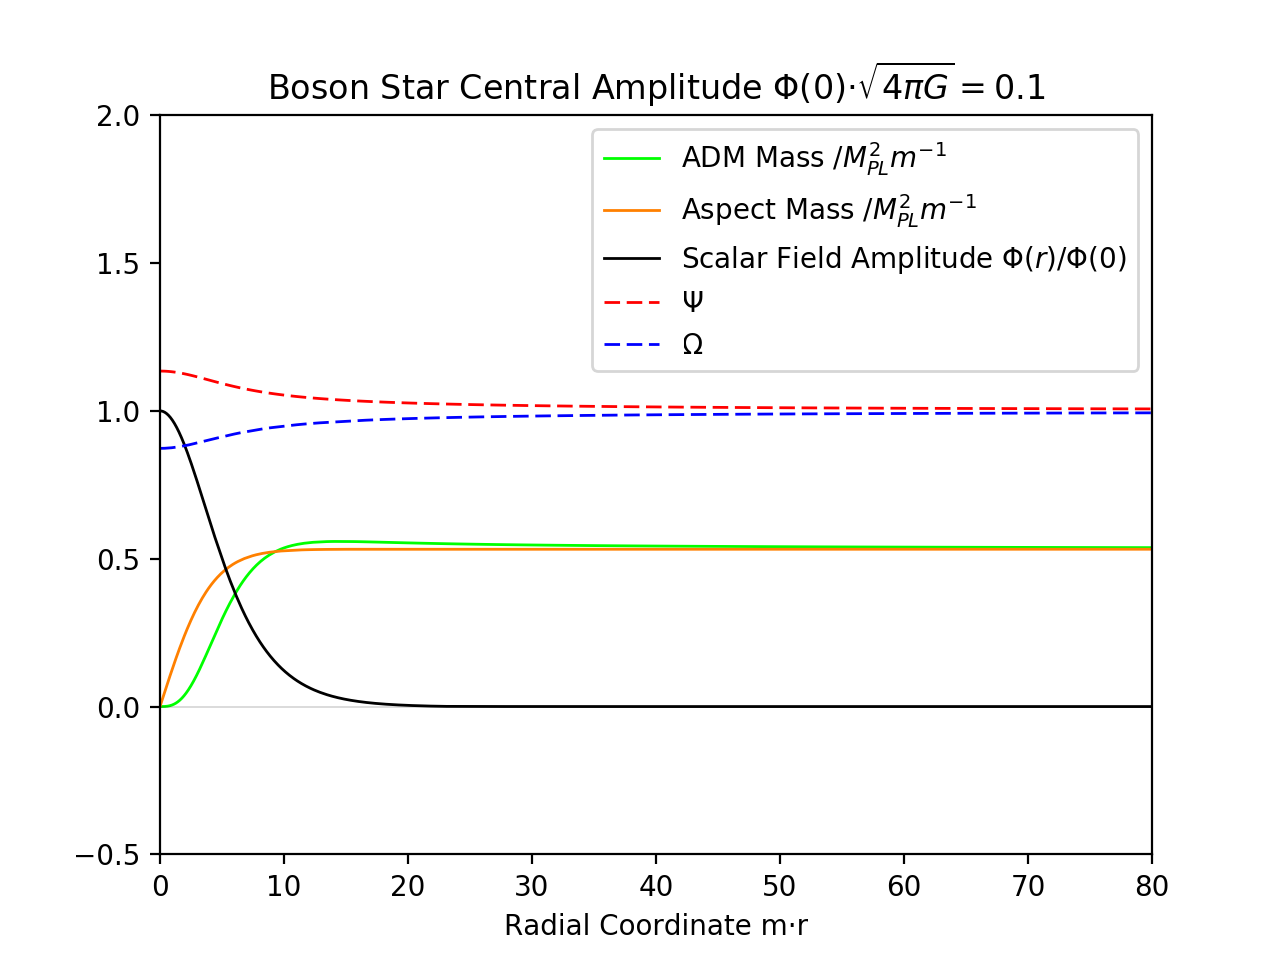
\includegraphics[width=0.5\textwidth]{png/bosonstar_groundstate.png}
%   %\hfill
%   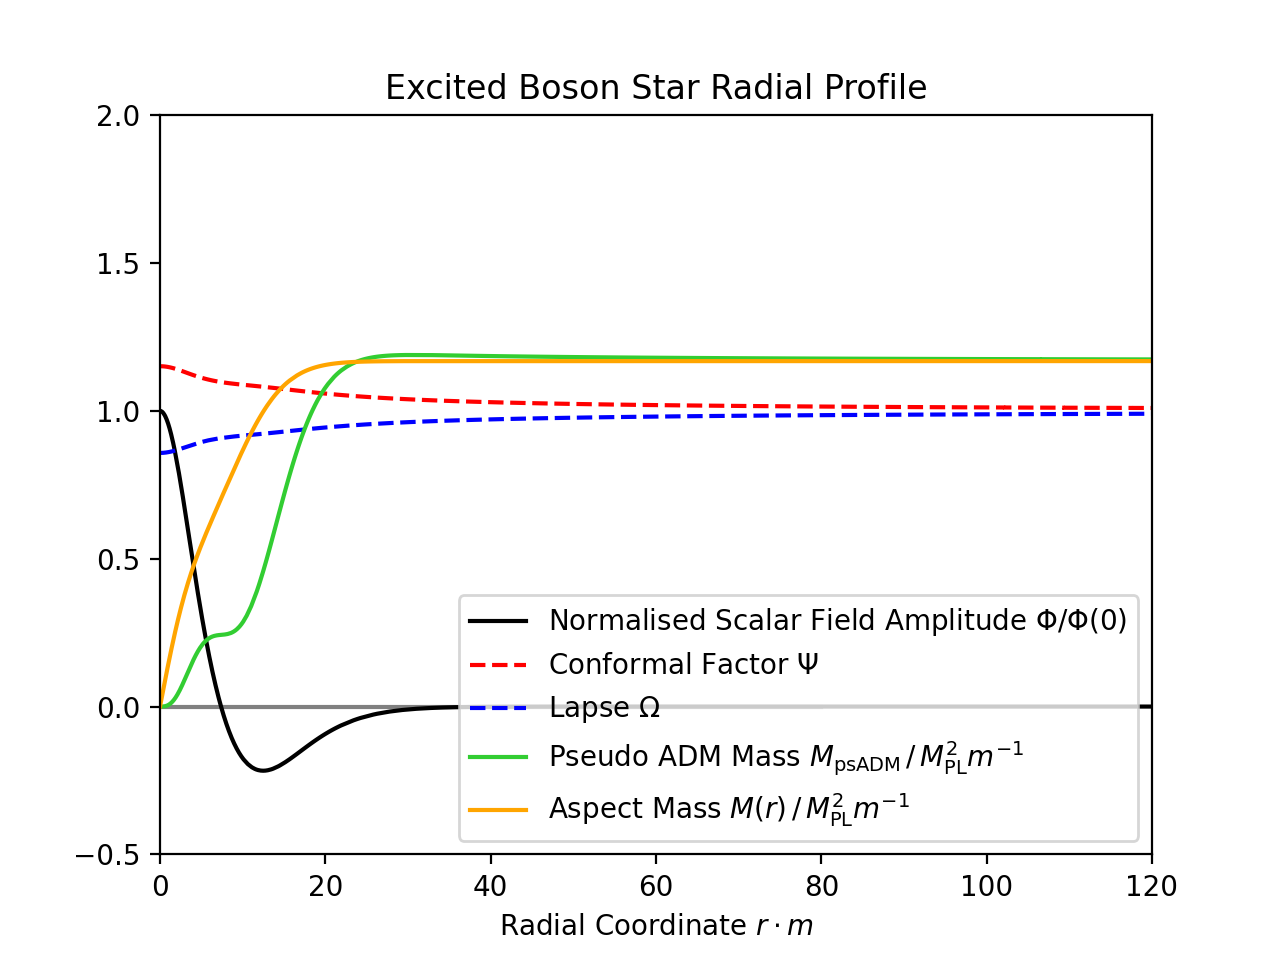
\includegraphics[width=0.5\textwidth]{png/bosonstar_excitedstate.png}
% \end{figure}

\begin{figure*}[h!]
    \subfloat%[\textsc{GRChombo}]
    {
        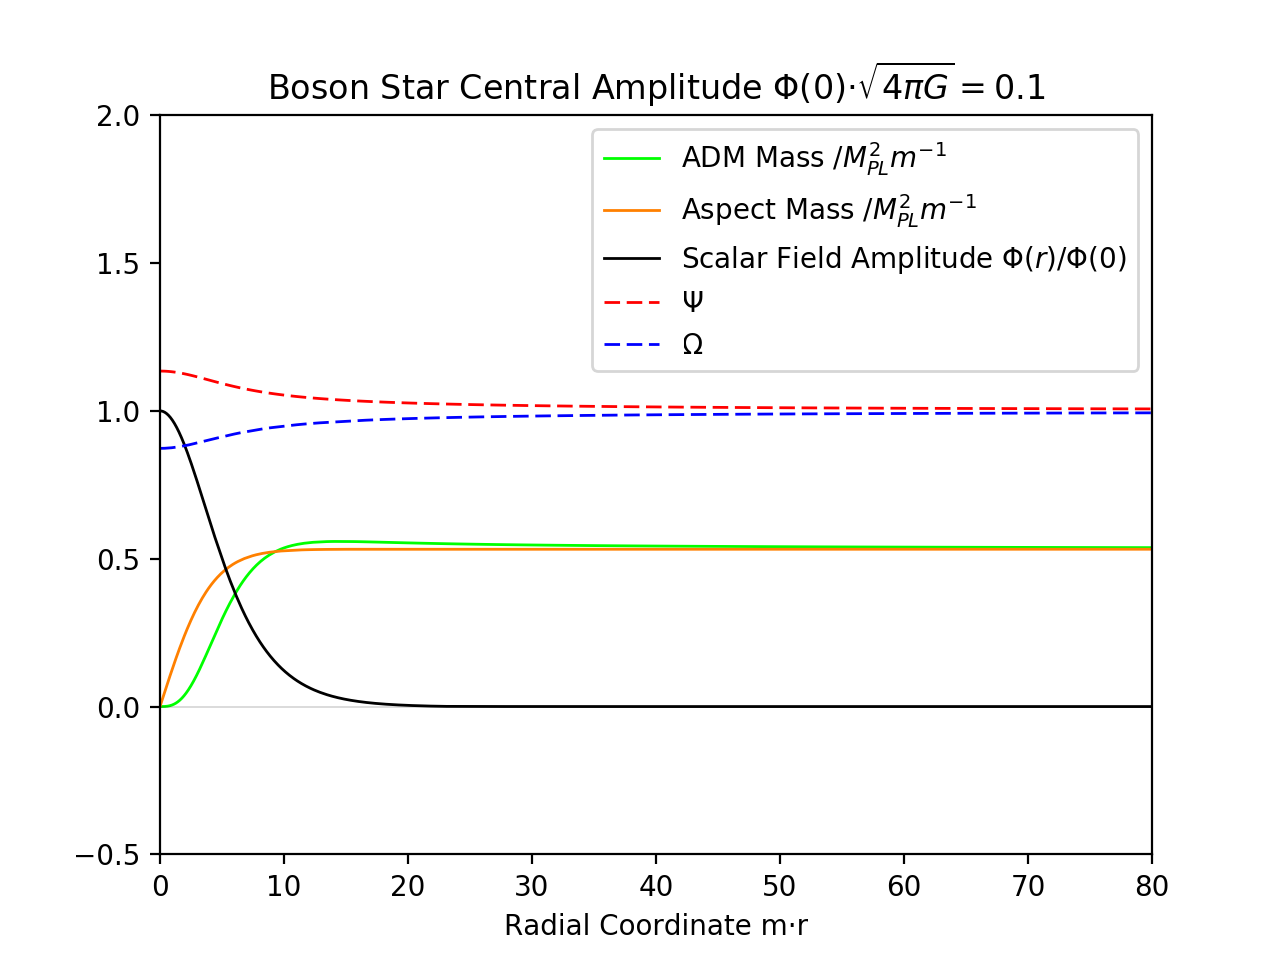
\includegraphics[width=0.48\linewidth]{png/bosonstar_groundstate.png}
        %\label{bhkick:fig:grchombo-convergence}
    }
    \hfill
    \subfloat%[\textsc{Lean}]
    {
        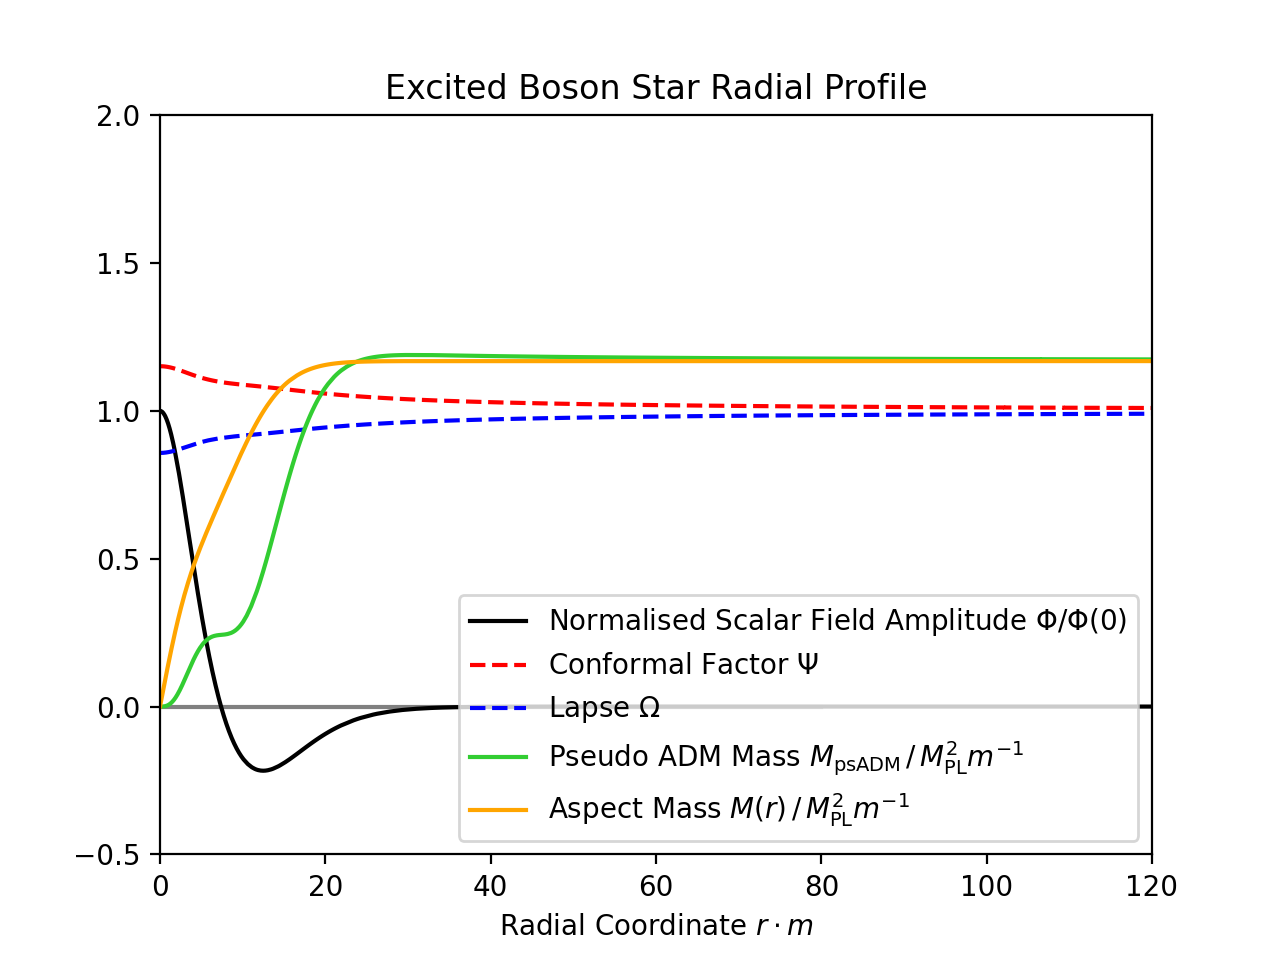
\includegraphics[width=0.48\linewidth]{png/bosonstar_excitedstate.png}
        %\label{bhkick:fig:lean-convergence}
    }
    \caption{Boson Star radial profile, Left: Ground state, Right: 1st Excited state. The ground state has an ADM mass of $M_{\rm ADM} = 0.532(5)~M_{\rm PL}^2 m^{-1}$ and the excited state has an ADM mass of $M_{\rm ADM} = 1.16(8)~M_{\rm PL}^2 m^{-1}$. Both stars have a central amplitude of $\Phi(0) \cdot \sqrt{4\pi G}=0.1 ~ m^{-1}$.
    The aspect mass is defined in Eq.~(\ref{malaise:eq:aspect_mass_def}) and the pseudo-ADM mass is given by Eq.~(\ref{boson:eq:admlike}); in the large radius limit, $M_{\rm psADM}(\infty) = M_{\rm ADM}$.}
    \label{boson:fig:f1}
\end{figure*}

%   \begin{figure}[h!]
%   \caption{Boson star radial profile for the ground state}
%   \centering
%   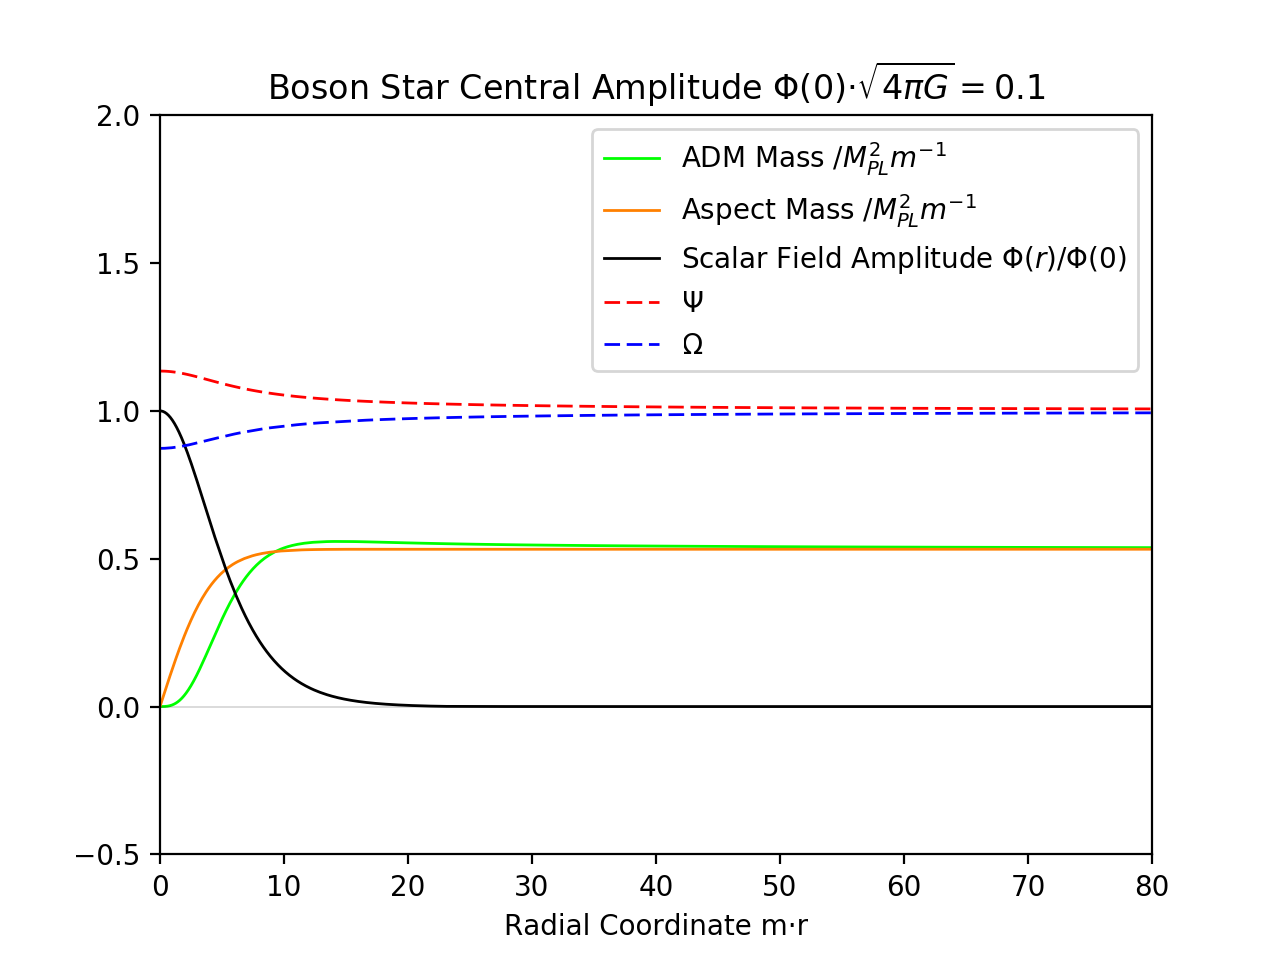
\includegraphics[width=0.8\textwidth]{png/bosonstar_groundstate.png}\label{boson:fig:f1}
% \end{figure}

%   \begin{figure}[h!]
%   \caption{Boson Star radial profile : 1st Excited state}
%   \centering
%   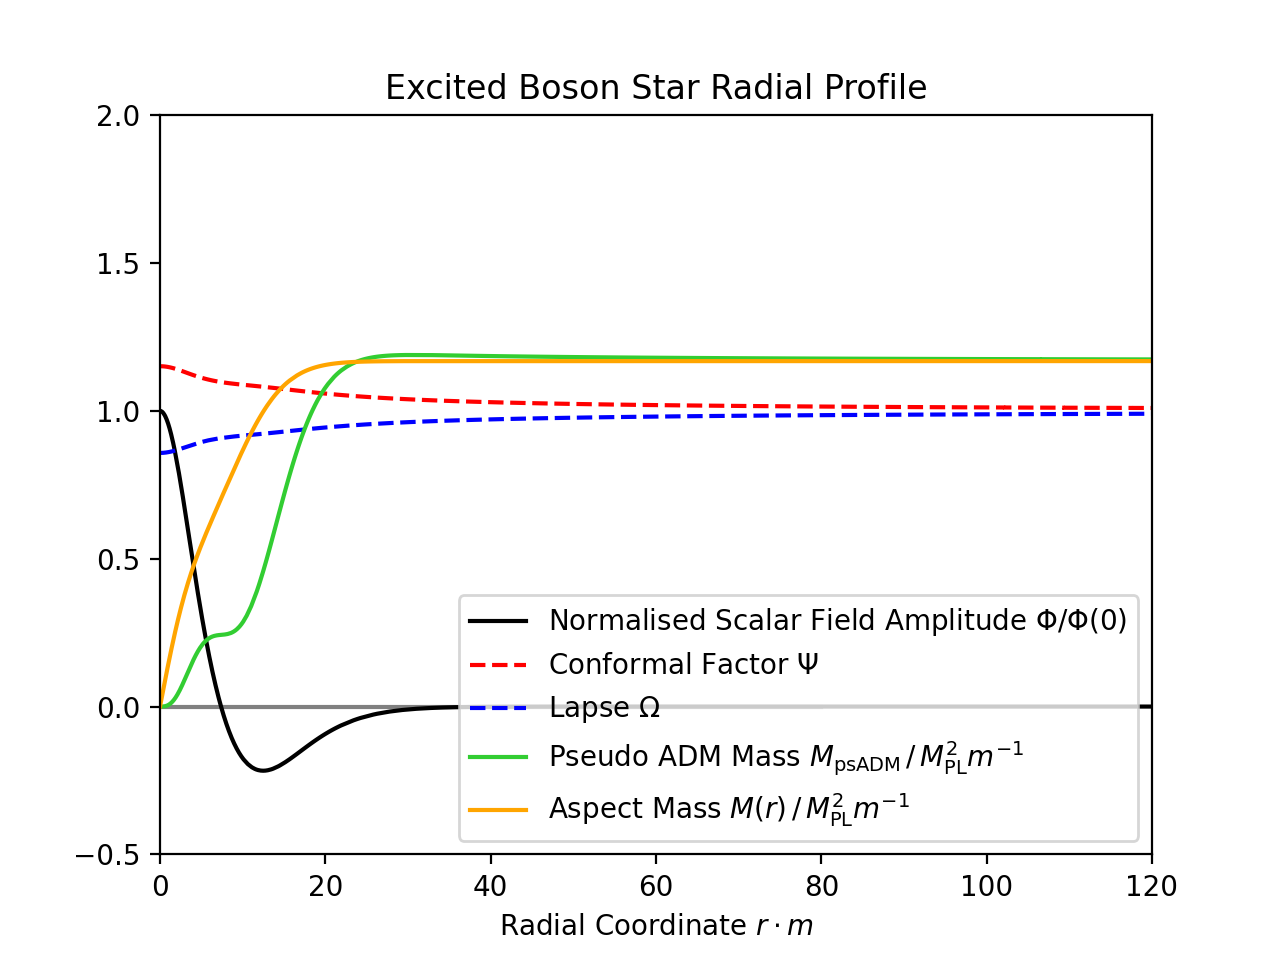
\includegraphics[width=0.8\textwidth]{png/bosonstar_excitedstate.png}\label{boson:fig:f2}
% \end{figure}


Putting everything together, a boson star solution with eigenvalue $\omega_0$
(or $\omega_n$ for excited stars) and asymptotic metric Eq.~(\ref{grchombo:eq:ABBB})
can be obtained. To find a star with asymptotic metric $\eta_{\mu\nu}$ of flat space,
the initial conditions are iteratively improved according to $\Omega_0 \rightarrow \Omega_0 /
\Omega_\infty$ and $\Psi_0 \rightarrow \Psi_0 / \Psi_\infty$; the interval bisection for
$\omega$ is then restarted. This is iterated three to five times which leaves $A=\Omega_\infty=1$
and $B=\Psi_\infty=1$ to high precision and the isotropic boson star profile has been created.
This whole process requires a few seconds runtime for a high resolution 500,000 gridpoint calculation on a regular laptop.


  \begin{figure}[h!]
  \caption{Boson star trends, Left: ADM mass vs $\Phi_0$, Right: ADM mass vs $r_{99}$}
  \centering
  \subfloat{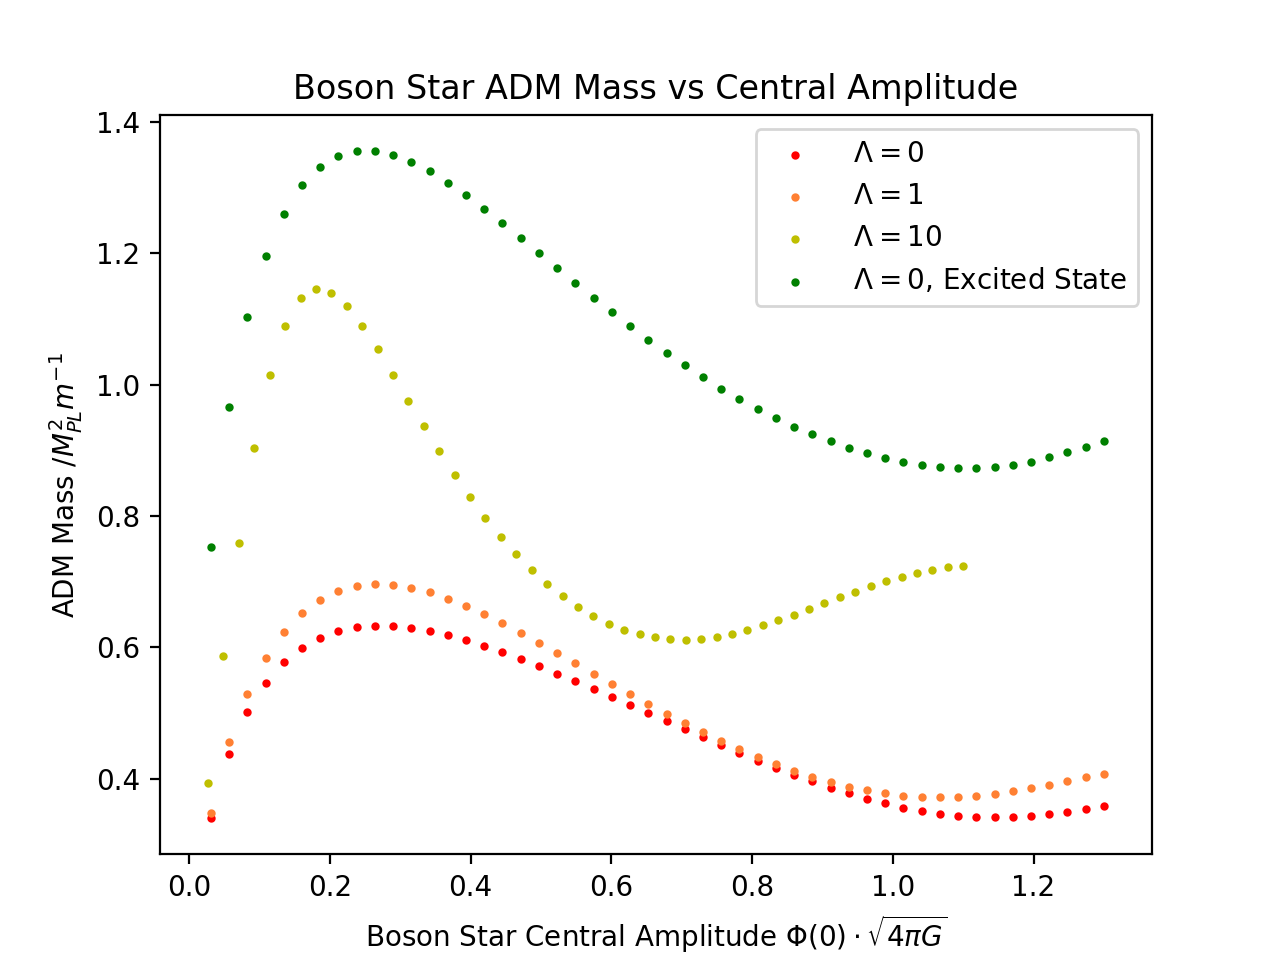
\includegraphics[width=0.48\textwidth]{png/ADM_vs_PC.png}}
  \hfill
  \subfloat{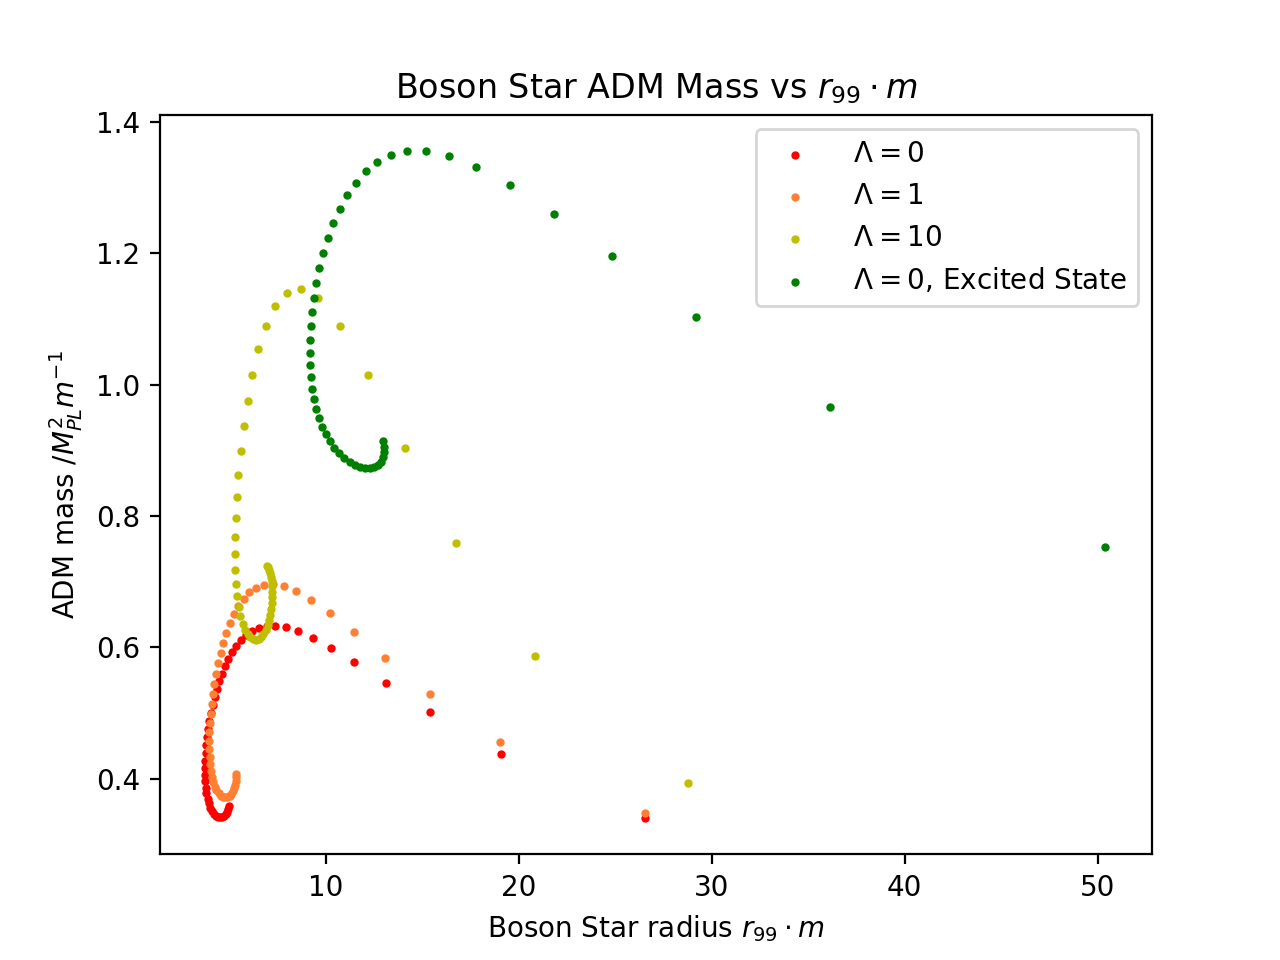
\includegraphics[width=0.48\textwidth]{png/ADM_vs_r99.png}}
  \label{boson:fig:f3}
\end{figure}

%   \begin{figure}[h!]
%   \caption{ADM mass vs $\Phi(0)$}
%   \centering
%   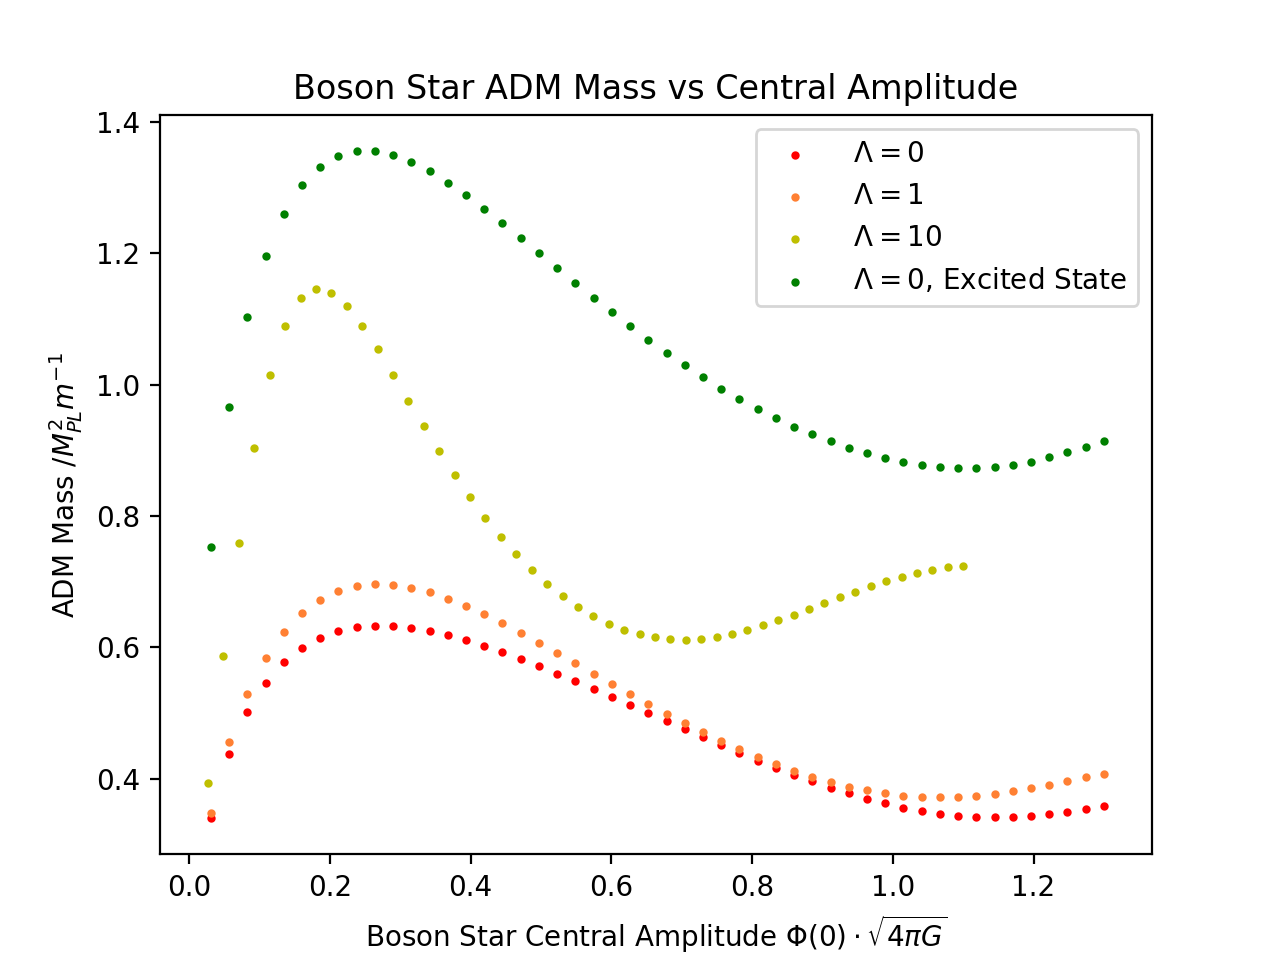
\includegraphics[width=0.8\textwidth]{png/ADM_vs_PC.png}\label{boson:fig:f1}
% \end{figure}

%   \begin{figure}[h!]
%   \caption{ADM mass vs $r_{99}$}
%   \centering
%   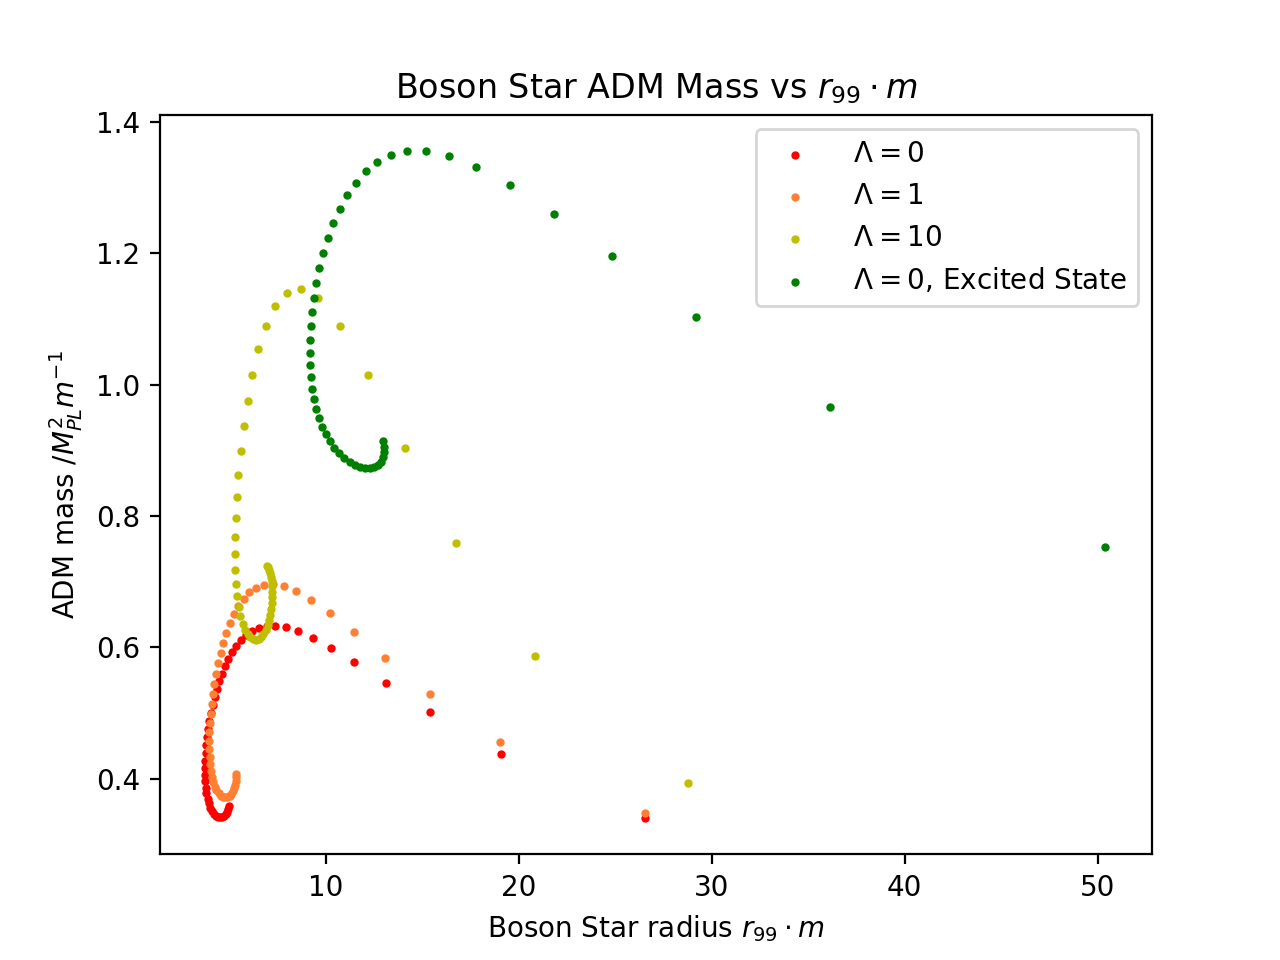
\includegraphics[width=0.8\textwidth]{png/ADM_vs_r99.png}\label{boson:fig:f2}
% \end{figure}



Figure~\ref{boson:fig:f1} shows the numerically obtained radial profile of a mini boson star ($\Lambda=0$) and an excited mini boson star. Note two mass definitions are plotted; the aspect mass defined in Eq.~(\ref{malaise:eq:aspect_mass_def}) and a pseudo-ADM mass. The conventional ADM mass \cite{arnowitt1962dynamics} is defined as
\begin{equation}
M_{\rm ADM} := \frac{1}{16\pi}\lim_{r\rightarrow\infty}\oint_{s_r} N^i \gamma^{jk}\left(\partial_j \gamma_{ik} - \partial_i \gamma_{jk} \right) \dd A,
\end{equation}
for radial coordinate $r$, 2-sphere $s_r$ of radius $r$ and unit normal vector $\bs{N}$. For an isotropic, diagonal, spherically-symmetric spatial metric ${\gamma}_{ij}$ with $\gamma_{rr} = \Psi^2(r) $, $\gamma_{\theta\theta}=\Psi^2(r)r^2$ and $\gamma_{\phi\phi}=\Psi^2(r)r^2 \sin^2\theta$ (in polar coordinates) this simplifies to,
\begin{align}
M_{\rm ADM} &= \frac{1}{16\pi}\lim_{r\rightarrow\infty}\oint_{s_r} \left(N^r \gamma^{rr}\partial_r \gamma_{rr} - N^r \gamma^{jk}\partial_r \gamma_{jk} \right) \dd A,\\
&= \frac{1}{16\pi}\lim_{r\rightarrow\infty}\oint_{s_r} N^r \Psi^{-2}\left( \partial_r \Psi^2 -  \delta^{jk}\delta_{jk}\partial_r \Psi^2 \right) \sqrt{\gamma_{\theta\theta} \gamma_{\phi\phi}} \dd \theta \dd \phi,\\
&= \frac{1}{16\pi}\lim_{r\rightarrow\infty}\int_{\theta=0}^{\theta=\pi}\int_{\phi=0}^{\phi=2\pi} -4 \Psi^{-2}\left(\partial_r \Psi \right) \Psi^2 r^2 \sin^2\theta \dd \theta \dd \phi,\\
&= \lim_{r\rightarrow\infty} \left(- r^2 \partial_r \Psi\right) ,\\
\end{align}
where we used the fact that $\bs{\gamma}(\bs{N},\bs{N})=1$ which gives $N^r = (\gamma_{rr})^{-1/2} = \Psi^{-1}$.
Note that for a Schwarzschild black hole with $\Psi = \left(1+\frac{M}{2r} \right)^2$ the ADM mass formula returns
the expected result of $M$. We define the {\it pseudo-AMD mass} as
\begin{equation}
M_{\rm psADM}(r):=- r^2 \partial_r \Psi ,\label{boson:eq:admlike}
\end{equation}
which of course satisfies $M_{\rm ADM} = M_{\rm psADM}(\infty)$.

 Polytropic fluid star initial data has also been calculated as a preliminary test
 of the code; they are easier to create as they do not require solving an eigenvalue
 problem and do not have an asymptotically growing mode. Figure~(\ref{boson:fig:f3})
 shows how the ADM mass of boson stars varies with central amplitude $\Phi_0$ and
 $r_{99}$, the radius which $\Phi(r_{99}) = \Phi_0/100$. It should be noted that
 the mini boson star (with $\Lambda =0$) case agrees with the known maximum mass,
 the Kaup limit \cite{PhysRev.172.1331} $M_{\rm max} \approx 0.633 {M_{\rm PL}^2}{m^{-1}}$
 with the largest mass being $ M_{\rm max} = 0.63299(3) {M_{\rm PL}^2}{m^{-1}} $
 corresponding to a central amplitude of $ \sqrt{4\pi G}(\Phi_0)_{\rm max} = 0.271(0)~m^{-1}$.



While many different boson stars have been computed to test the initial data code,
all the following evolutions use the same boson star with parameters $\Lambda=0$,
$\sqrt{4\pi G}\Phi_0=0.1~m^{-1} \rightarrow \Phi_0 \approx 0.0282~m^{-1}$ and
ADM mass $M=0.532(7)~M_{\rm PL}^2 m^{-1}$. This is as the stars are heavy enough
to form black holes under collisions and large deformations, but stable enough
to not collapse to a black hole for moderate perturbations.




\subsection{Single Star Evolution}

As a check that the initial data from section \ref{grchombo:sec:initialdata} is correct,
a mini boson star with central density $\Phi_0=0.02820~m^{-1}$ is evolved in time
in three spatial dimensions. The simulation has a physical domain size $L=1024~m^{-1}$
with $N=320$ gridpoints on AMR level zero with grid spacing $\Delta x = 3.2~m^{-1}$.
The AMR is allowed up to six extra levels; the finest level (level six) has a grid
spacing of $\Delta x = 0.05~m^{-1}$. The star is supposed to remain in the centre
of the grid and not change as it is a rest frame soliton; this is observed through
evolution with {\sc GRChombo}. Figure (\ref{boson:fig:f5}) shows the global maximum
value of $|\vp|$ (left figure) and the total integral of the Noether charge ${N}$
over the grid (right figure). As can be seen, $|\vp|_{\rm max}$ is constant to
$\sim 0.7\%$ and $N$ is conserved to the $\sim 0.07\%$ level until time $t=320~m^{-1}$.

  \begin{figure}[h!]
  \caption{Left: Maximum of $|\vp|$ during the evolution, Right: Total integrated Noether charge $N$.
  The initial noise seen in the two figures is attributed to junk radiation from
  refinement boundaries and is potentially exacerbated by the gauge settling from
  the initial gauge to the moving puncture gauge used. The lower-amplitude oscillation
  seen continuously in the left figure is due to finite resolution when calculating
  the maximum value $\varphi_{\rm max} = [{\rm Re}(\varphi)^2 + {\Im}(\varphi)^2]_{\rm max}$
  on any gridpoint. }
  \centering
  \subfloat{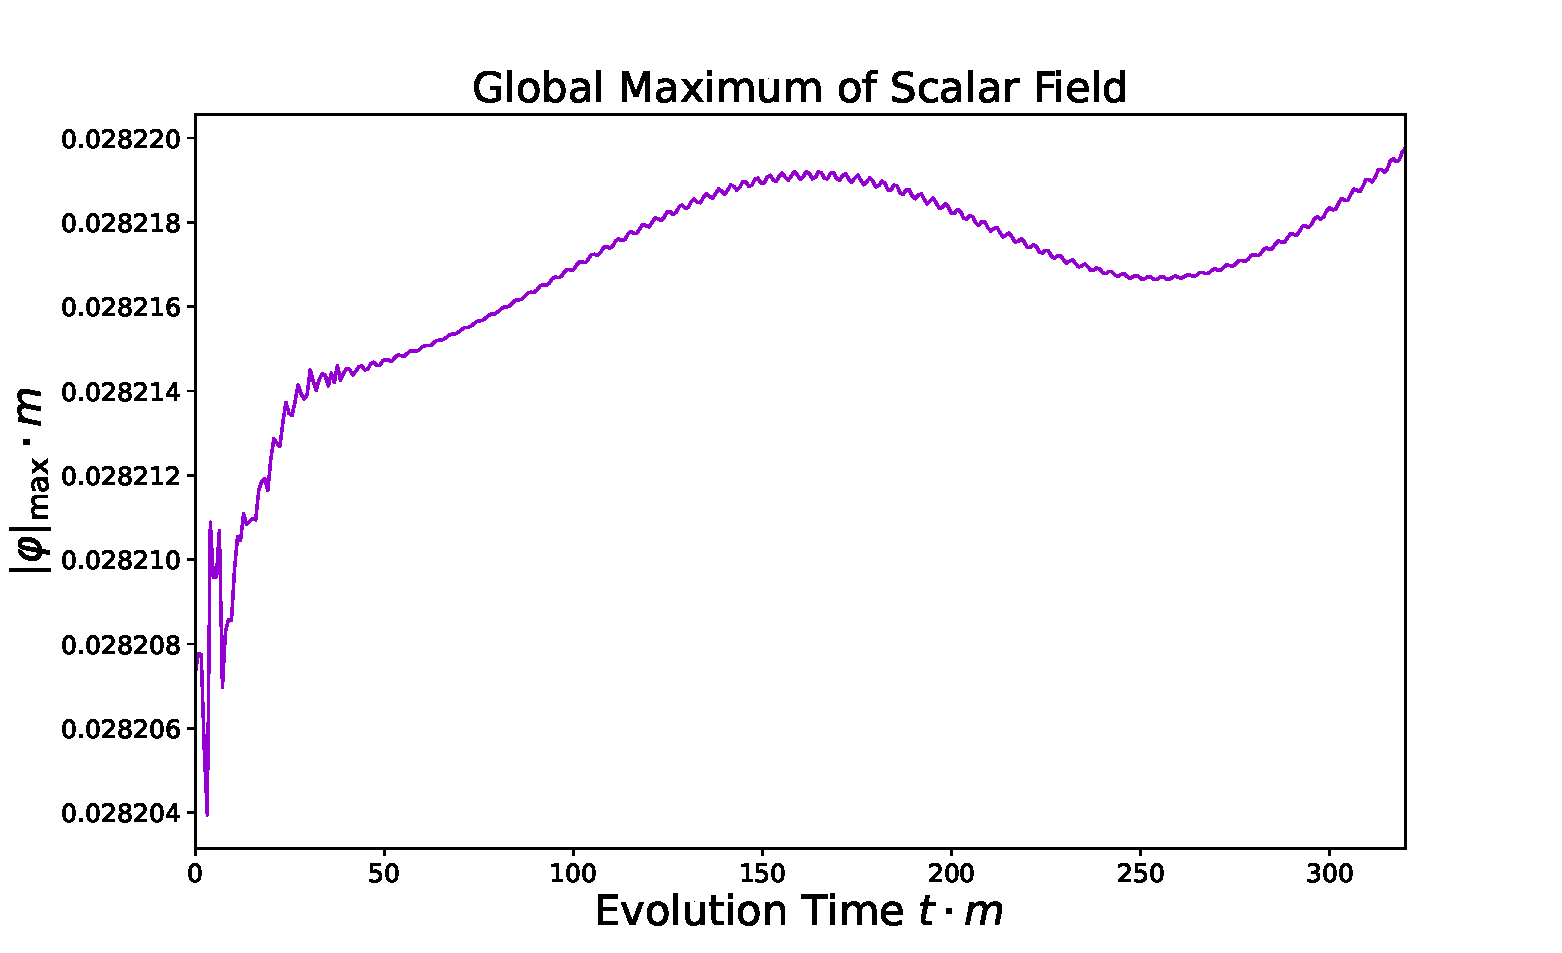
\includegraphics[width=0.5\textwidth]{data/star_modphi_nicer.pdf}}
  \hfill
  \subfloat{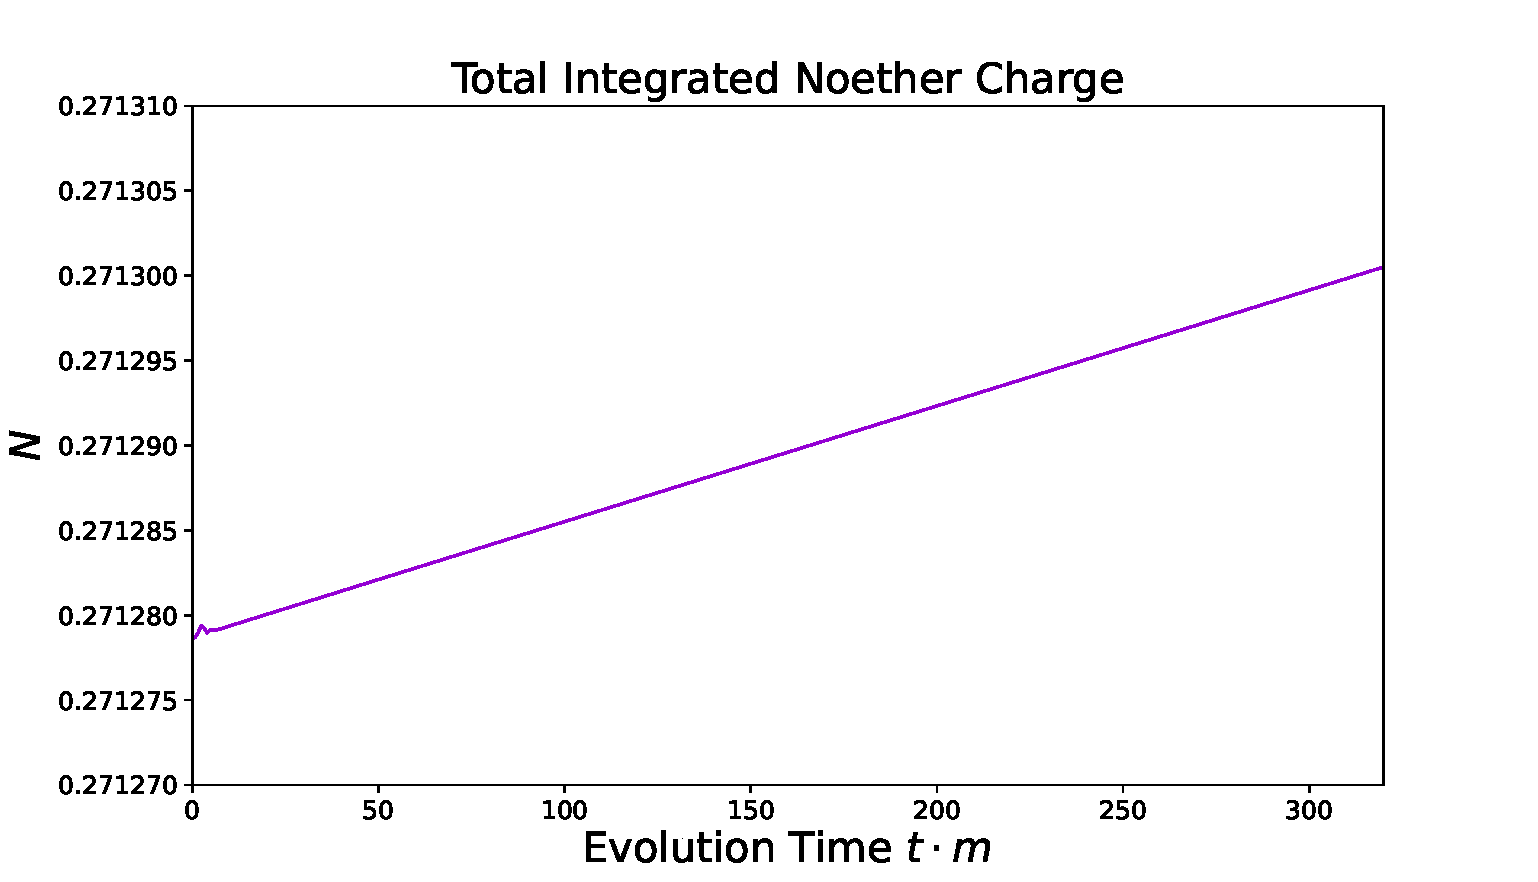
\includegraphics[width=0.5\textwidth]{data/star_N_nicer.pdf}}
  \label{boson:fig:f5}
\end{figure}






\subsection{Superposition of Initial Data} \label{grchombo:sec:superposition}
In order to simulate a spacetime consisting of two stars (or a star and a black hole) we must choose a way of superposing the initial data of two objects, centred at $x^{(1)}$ and $x^{(2)}$. For some field $\psi^{(j)}$ associated with the compact object at $x^{(j)}$,
\begin{equation}
\psi^{(j)} = \psi(x-x^{(j)}),
\end{equation} where $\psi$ refers to the object centred about the origin.
Taking two compact objects with fields $\vp$, $\Pi$, $\gamma_{ij}$, $\K_{ij}$, $\alpha$ and $\beta^i$, a naive superposition scheme was chosen;
\begin{align}
 \vp &= \vp^{(1)} + \vp^{(2)},\\
\Pi &= \Pi^{(1)} + \Pi^{(2)},\\
 \K^i_j &= {\K^{(1)}}^i_j+{\K^{(2)}}^i_j,\\
 \gamma_{\mu\nu} &= \gamma^{(1)}_{\mu\nu} + \gamma^{(2)}_{\mu\nu}-\delta_{\mu\nu},\\
\beta_i &= \beta^{(1)}_i + \beta^{(2)}_i ,\\
 \alpha &= \sqrt{\alpha_{(1)}^2 + \alpha_{(2)}^2-1},\\
 \chi &= \det\left(\gamma^{(1)}_{\mu\nu} + \gamma^{(2)}_{\mu\nu}-\delta_{\mu\nu}\right)^{-1/3},
 \end{align}
where the super-scripts ${}^{(1)}$ and ${}^{(2)}$ refer to the separate compact objects. The extrinsic curvature is chosen to be superposed with mixed indices so that it implies the trace $\mathcal{K}$ is also superposed. If one of the compact objects is a black hole the lapse $\alpha \rightarrow 0$ on the horizon; this is circumvented by setting,
\begin{equation} \alpha = \sqrt{\chi},\end{equation}
ensuring that the lapse is real and non-negative everywhere on $\Sigma_t$.

Superposing two solutions in general relativity usually no longer satisfies the Einstein equation; the Hamiltonian constraint Eq.~(\ref{nr:eq:ham}) and momentum constraints Eq.~(\ref{nr:eq:mom}) are violated. For asymptotically flat compact objects, the constraint violation reduces to zero as the object separation tends to infinity. In the case of finite separations, the CCZ4 scheme in section \ref{nr:sec:ccz4} aims to drive the constraint violation towards zero and hence a true solution of Einstein's equation; in practice, the CCZ4 scheme is more efficient at damping low amplitude, high-frequency violations and will not fully reduce long-wavelength violations \cite{gundlach2005constraint}. The collisions of compact objects in section \ref{grchombo:sec:bscollisions} use this naive superposition scheme. Section \ref{mal:sec:improvedsuperposition} explores a technique to improve the naive superposition of compact objects.



















\subsection{Collisions of Boson Stars}\label{grchombo:sec:bscollisions}



Both a headon collision and a grazing collision of two boson stars are simulated
using the superposition scheme given in section \ref{grchombo:sec:superposition}.
The two stars are identical, each has a central density of $\Phi_0=0.02820~m^{-1}$
and an ADM mass $M=0.532(7) ~M_{\rm PL}^2m^{-1}$. The stars are placed at positions
$x^i=\pm\{40,0,0\}~m^{-1}$ in the headon case and $x^i=\pm\{40,8,0\}~m^{-1}$ in
the grazing case and are boosted together with respective velocities $v^i=\mp\{0.1,0,0\}$
in both cases. A speed of $v=0.1$ corresponds to a rapidity of $\psi=0.1003353$.
The simulations have a physical domain size of $L=512~m^{-1}$ with $N=256$ gridpoints
on AMR level zero, this gives a coarse grid resolution of $\Delta x = 2~m^{-1}$.
There are up to five extra AMR levels giving a finest grid resolution of $\Delta x = 1/16~m^{-1}$.




\subsubsection{Headon Collision}
 \begin{figure}[h!]
  \caption{Left: Maximum of $|\vp|$ during evolution, Right: Total integrated Noether charge $N$.}
  \centering
  \subfloat{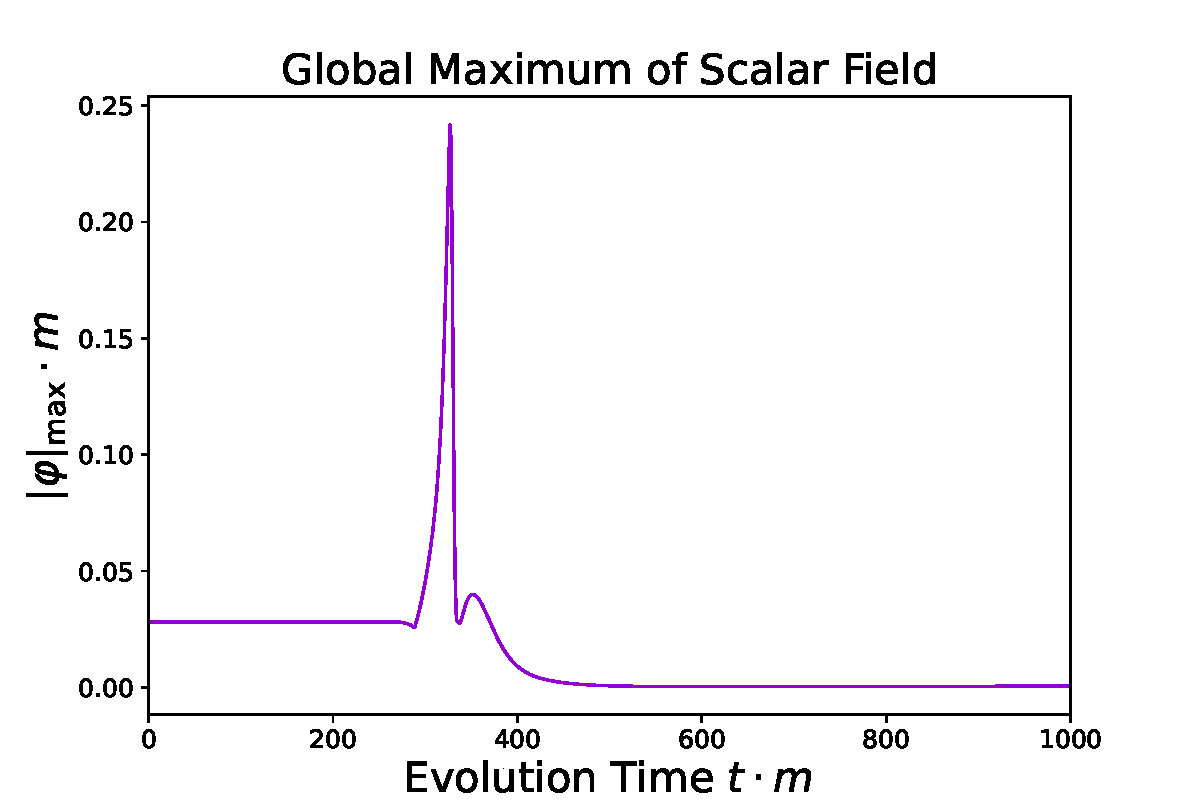
\includegraphics[width=0.5\textwidth]{data/headon_modphi_nicer.pdf}}
  \hfill
  \subfloat{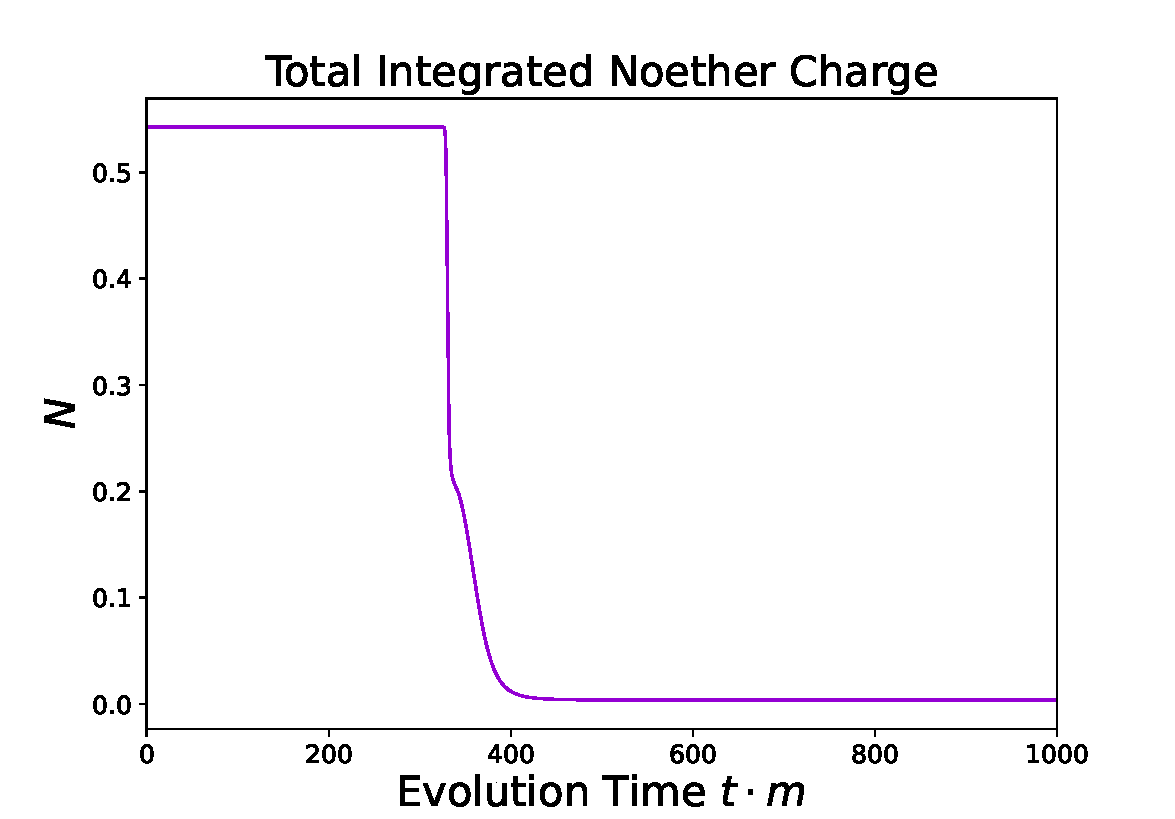
\includegraphics[width=0.5\textwidth]{data/headon_N_nicer.pdf}}
  \label{boson:fig:f7}
\end{figure}

\begin{figure}[h!]
  \caption{Gravitational wave signal of the headon boson star collision. The $l,m=2,2$ and $l,m=2,0$ spin weighted spherical harmonic modes of the $\Psi_4$ Newman-Penrose scalar are given.}
  \centering
  \subfloat{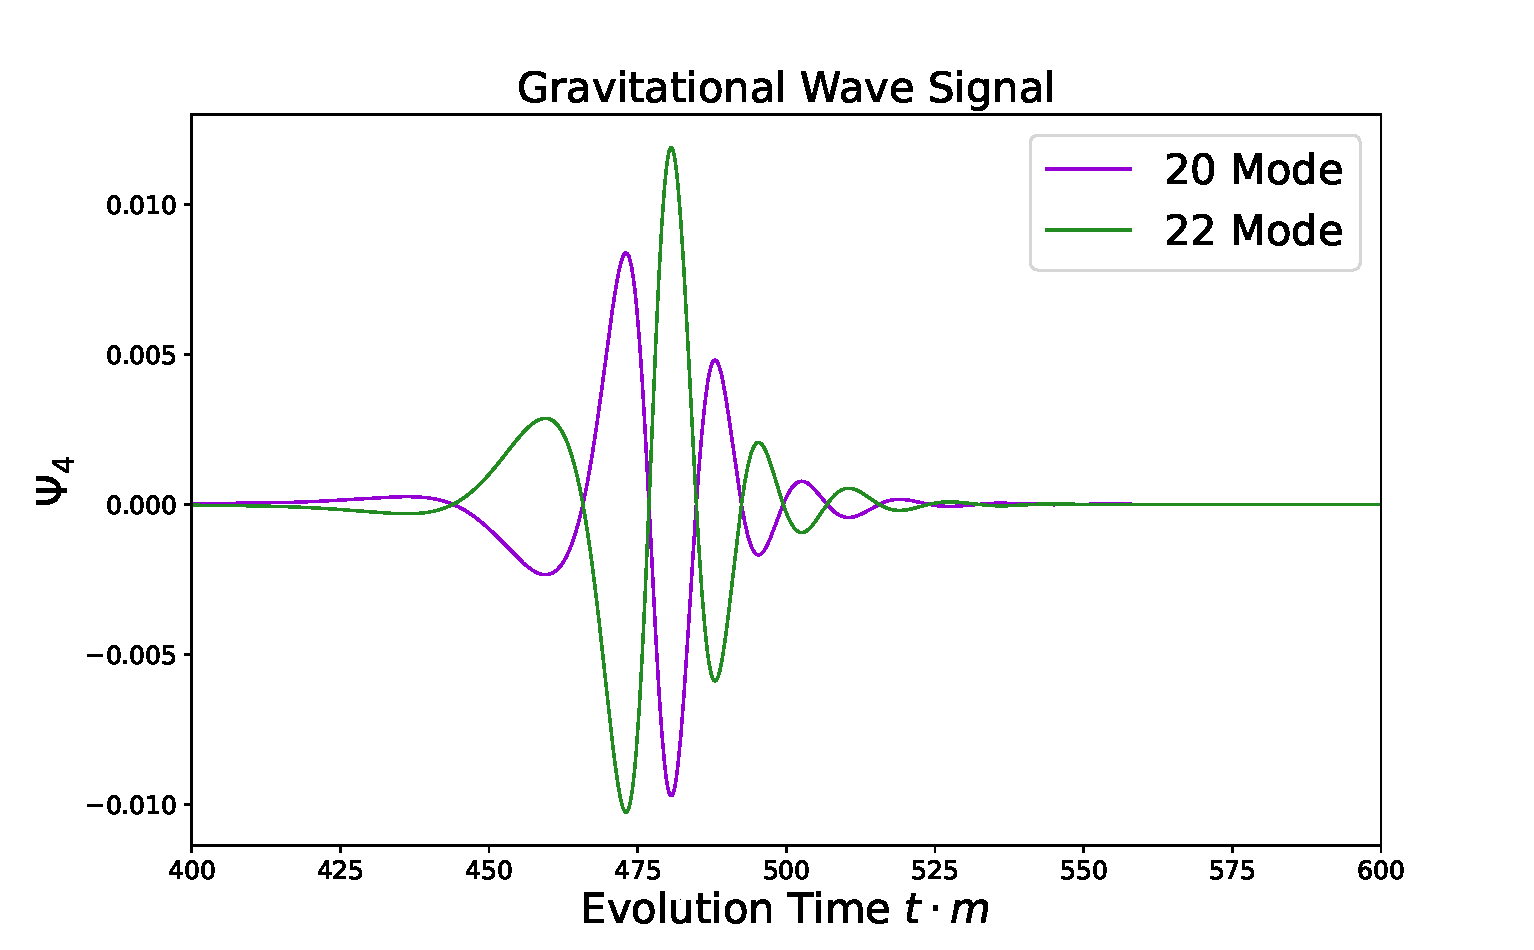
\includegraphics[width=0.5\textwidth]{data/headon_weyl_nicer.pdf}}\label{boson:fig:f9}
\end{figure}

Figure (\ref{boson:fig:f7}) shows $|\vp|_{\rm max}$, the global maximum value of $|\vp|$, and the total Noether charge $N$ as a function of time for the headon collision. At time $t\approx 289 ~m^{-1}$, $|\vp|_{\rm max}$ rapidly increases and then drops to zero, signalling the collapse to a black hole. At time $t\approx 327~m^{-1}$, there is a temporal maximum in $|\vp|_{\rm max}$ as the resolution limit of the simulation is reached and the scalar field is dissipated by the Kreiss-Oliger dissipation and diverging resolution requirements. This dissipation can also be seen in the Noether charge plot at a time of $t \approx 326~m^{-1}$ where the total charge that should remain constant but begins to fall. The lack of sufficient resolution inside the black hole is however not problematic for the external simulation; the errors accumulated are trapped inside the event horizon. Figure~(\ref{boson:fig:f7}) shows that the total Noether charge rapidly decays to zero at late time as it falls into the black hole and is dissipated.


The gravitational wave extraction at radius $r=140~m^{-1}$ is given in figure \ref{boson:fig:f9}. A spin-weighted spherical harmonic decomposition of the Newman-Penrose scalar $\Psi_4$ has been done and the $l,m = 2,0$ and $l,m = 2,2$ modes are plotted.


The dynamics of the two boson stars are shown in Fig.~(\ref{boson:fig:ff7}) which plots the scalar field modulus $|\vp|$ in the $x,y$ plane. The stars collide at time $275~m^{-1} < t < 300~m^{-1}$; which compares well to the Newtonian collision time\footnote{A simulation of point masses in Newtonain physics has been done to extract a collision time.} $t = 287.6~m^{-1}$ of two point masses with the same initial conditions. Soon after collision, an over-density of the scalar field develops which subsequently collapses to a black hole. The black hole then accretes the surrounding scalar field; the scalar field can be seen to be composed of higher order spherical harmonic modes at later times.






\subsubsection{Grazing Collision} \label{grchombo:sec:graze}

Figure (\ref{boson:fig:f10}) plots $|\vp|_{\rm max}$ and the total Noether charge
($N$) versus time for the grazing collision. At time $t\approx 309~m^{-1}$,
$|\vp|_{\rm max}$ rapidly increases and a black hole is soon formed. The black
hole is assumed\footnote{\color{orchid} No horizon measure, or measure of angular
momentum of matter
falling into the black hole, has been done for this simulation -
these measures would be warranted in any future study.}
to be spinning due to the collapsing matter containing angular
momentum. At time $t\approx 356 ~m^{-1}$ there is a temporal maximum in $|\vp|_{\rm max}$;
similarly to the headon collision, this is caused by diverging resolution requirements
near the black hole centre and does not affect the exterior spacetime. Consequently,
the Noether charge plot shows a drop in charge at a time of $t \approx355~m^{-1}$.
 \begin{figure}[h!]
  \caption{Left: Maximum of $|\vp|$ during evolution, Right: Total integrated Noether charge $N$.}
  \centering
  \subfloat{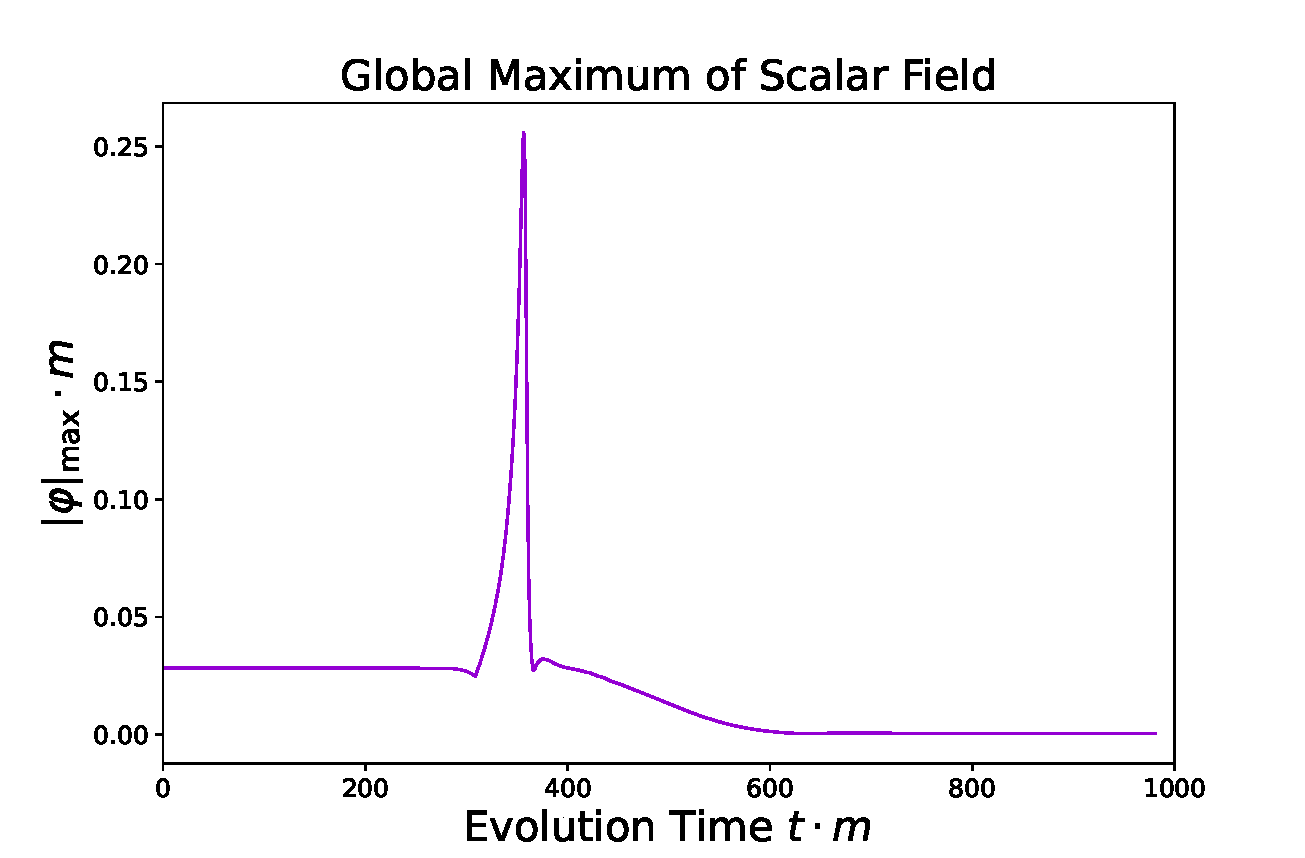
\includegraphics[width=0.5\textwidth]{data/graze_modphi_nicer.pdf}}
  \hfill
  \subfloat{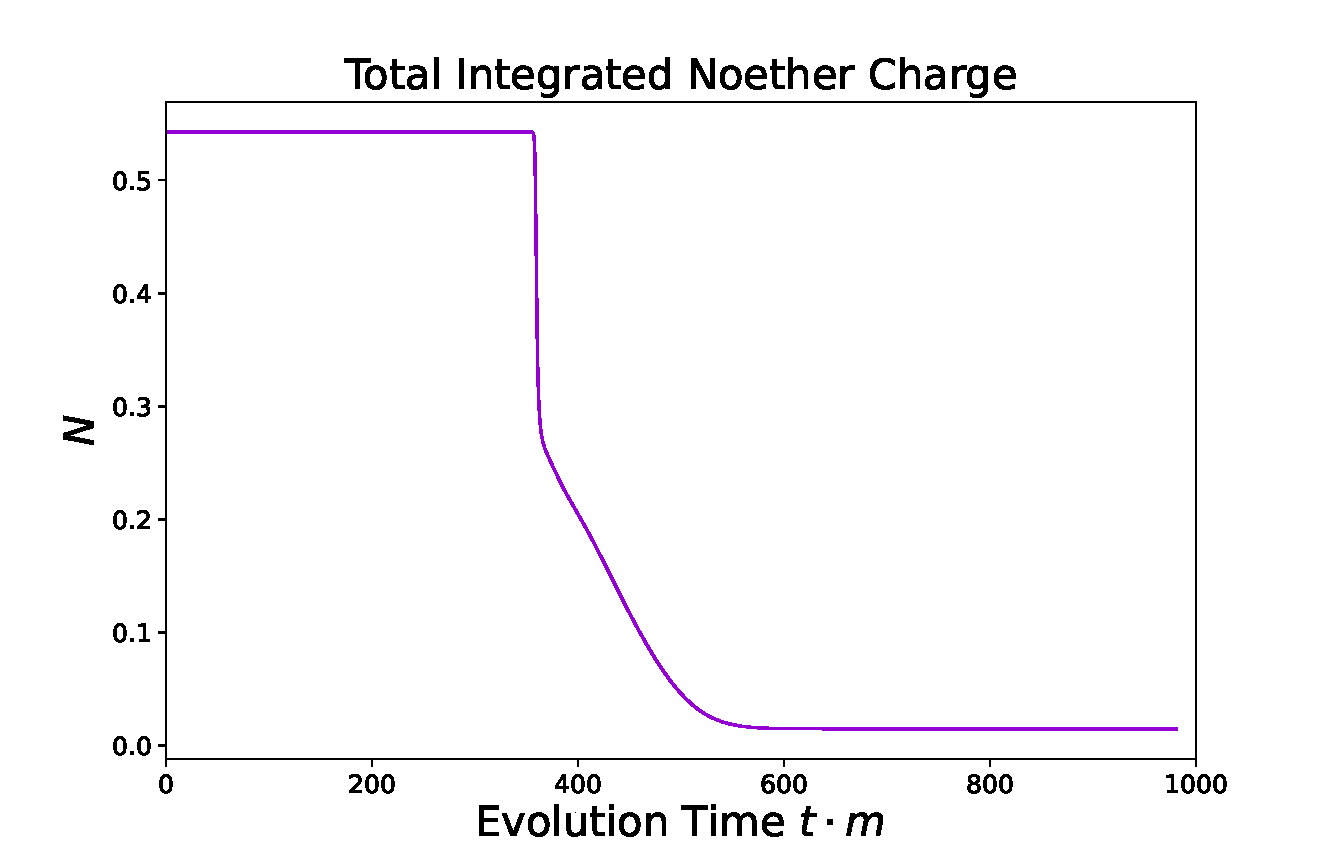
\includegraphics[width=0.5\textwidth]{data/graze_N_nicer.pdf}}
  \label{boson:fig:f10}
\end{figure}



A simulation of the grazing collision with point masses has been done using Newtons laws. The time taken for closest approach (with separation $s = 2.33~m^{-1}$) is $t=315.8~m^{-1}$; at this separation the finite sized stars would collide. Snapshots of the grazing boson star collision using numerical relativity (in full general relativity) are shown in Fig.~(\ref{boson:fig:ff10}) plotting the scalar field modulus $|\vp|$ in the $x,y$ plane. The stars collide at time $300~m^{-1} < t < ~m^{-1}$ which is in good agreement with the Newtonian approximtion. Soon after collision, an over-density of the scalar field develops and collapses to a black hole; this black hole is thought to be spinning due to the angular momentum of the collapsing matter. The black hole subsequently accretes most of the surrounding scalar field leaving a quasi-long-lived rotating toroidal scalar field configuration surrounding the black hole. This late time toroidal scalar field configuration will be referred to as a {\it toroidal wig} due to it being \enquote{fake} hair. The late time toroidal wig seems to settle to a rotationally symmetric configuration, with no quadrupole moment, and does not emit a significant gravitational wave signal; this can be seen in Fig.~(\ref{boson:fig:f12}) which plots the $l,m=2,2$ and $l,m=2,0$ modes of $\Psi_4$.



\begin{figure}[h!]
  \caption{Gravitational wave signal of the grazing boson star collision. The $l,m=2,2$ and $l,m=2,0$ modes of the $\Psi_4$ Newman-Penrose scalar are given.}
  \centering
  \subfloat{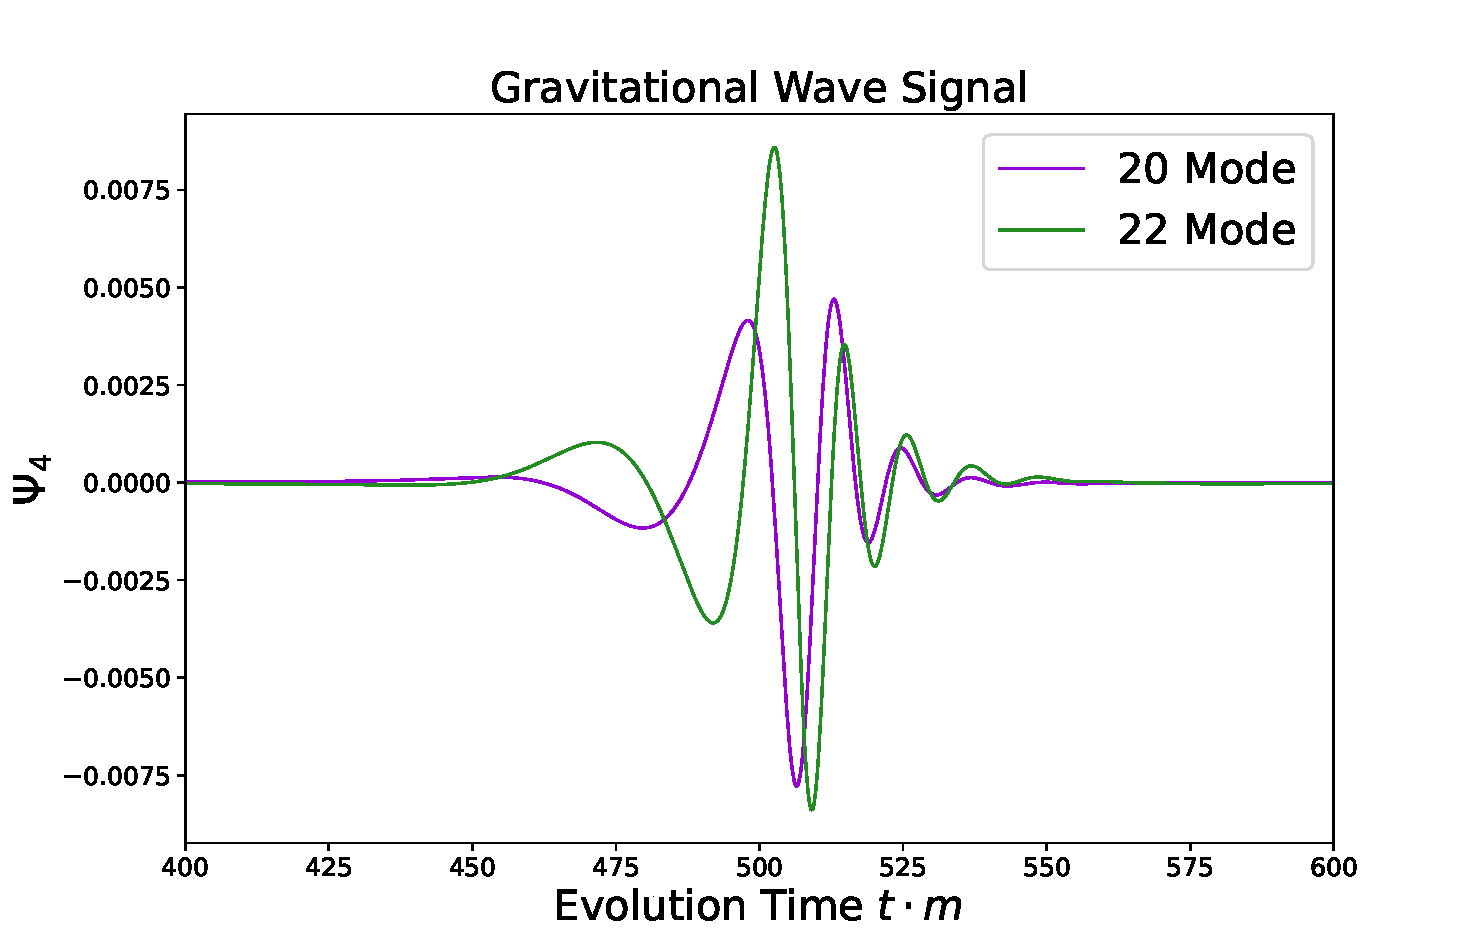
\includegraphics[width=0.5\textwidth]{data/graze_weyl_nicer.pdf}}
  \label{boson:fig:f12}
\end{figure}

 \begin{figure}[h!]
\caption{Left: Comparison of late time Noether charge $N$ between headon collision and grazing collision of two boson stars. Right: Late time plot of the Noether charge of the grazing collision only.}
\subfloat{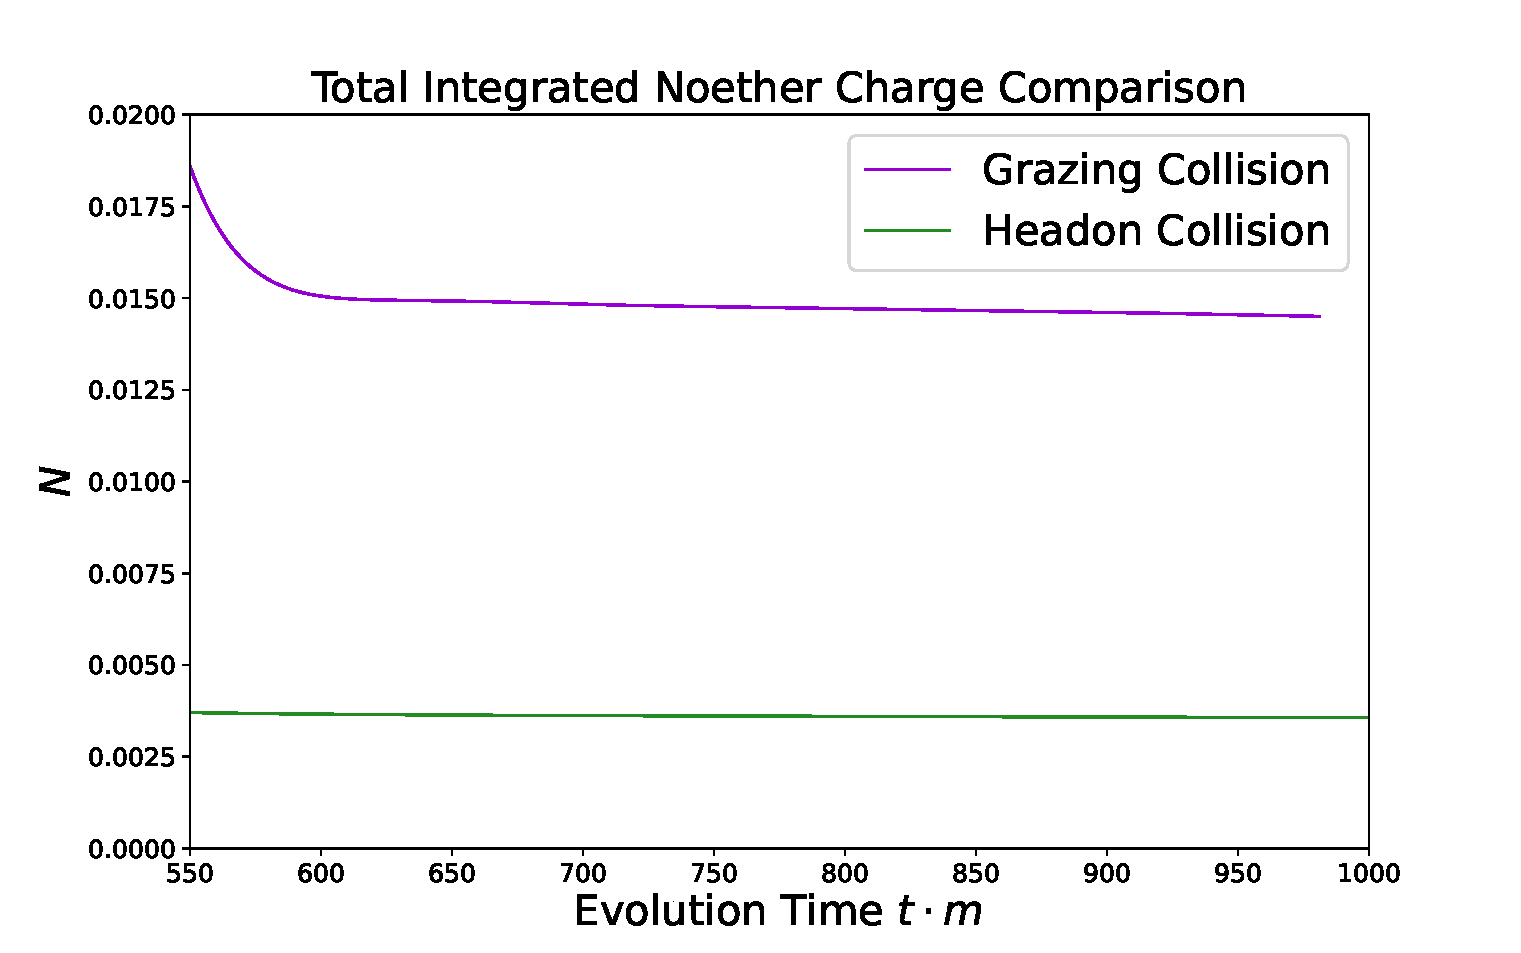
\includegraphics[width=0.45\textwidth]{data/late_time_N_nicer.pdf}}
\subfloat{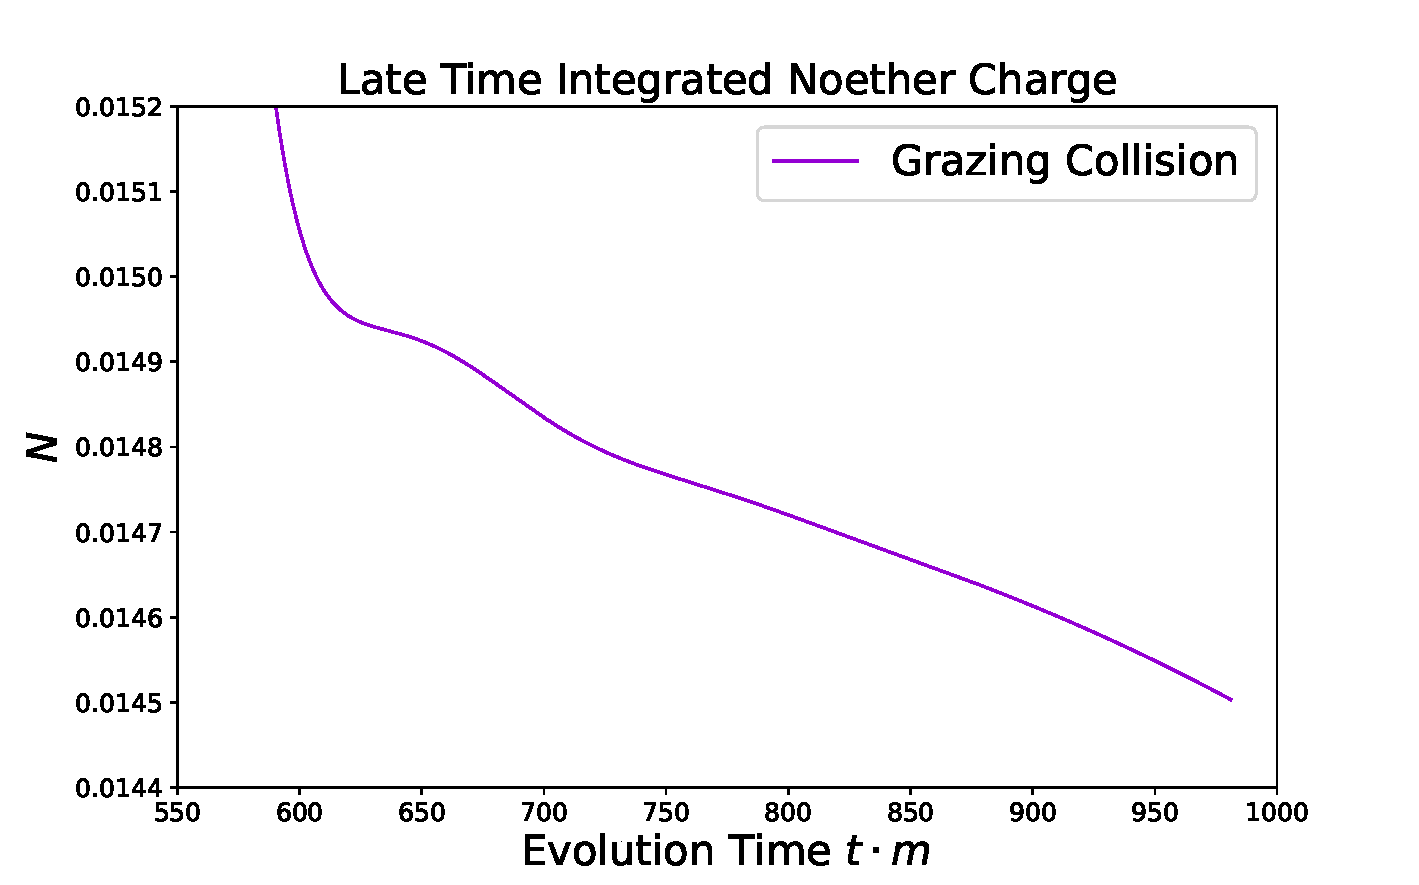
\includegraphics[width=0.45\textwidth]{data/noether_zoom_nicer.pdf}}
\label{boson:fig:fff}
\end{figure}



Figure (\ref{boson:fig:fff}) shows the late time Noether charge of the grazing and headon collisions. In contrast to the headon collision, the decay of $N$ in the grazing case is slower and reaches a value approximately $7$ times greater. Using linear extrapolation, the Noether charge of the grazing collision decays to zero at time $t \approx 12500 ~m^{-1} $ and hence the toroidal wig has an approximate lifespan of $12000~m^{-1}$.





 \begin{figure}[h!]
  \subfloat{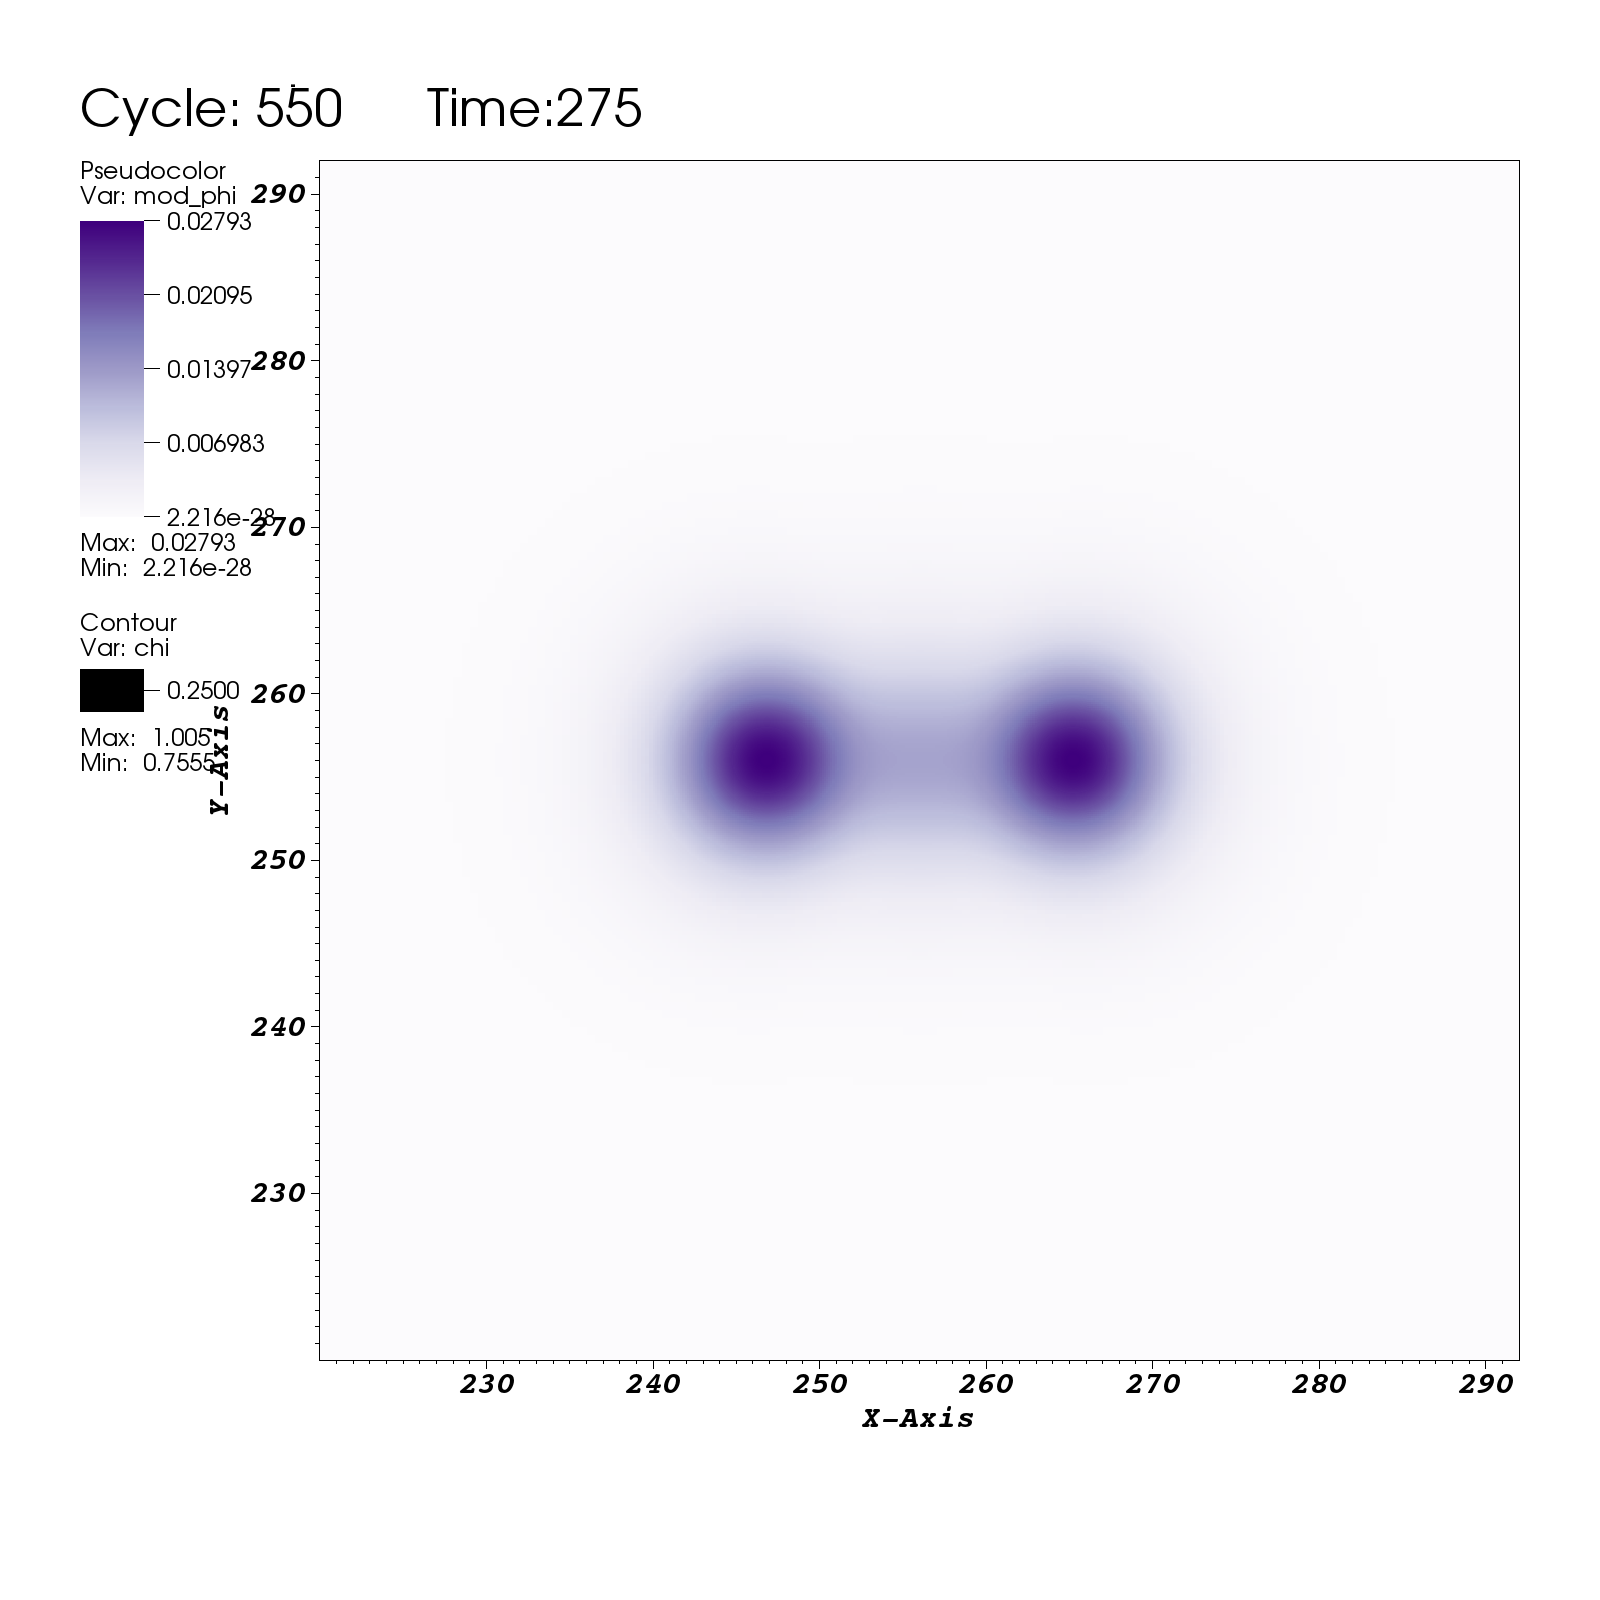
\includegraphics[width=0.50\textwidth]{modphi/headon_mod_phi0011.png}}\hfill
  \subfloat{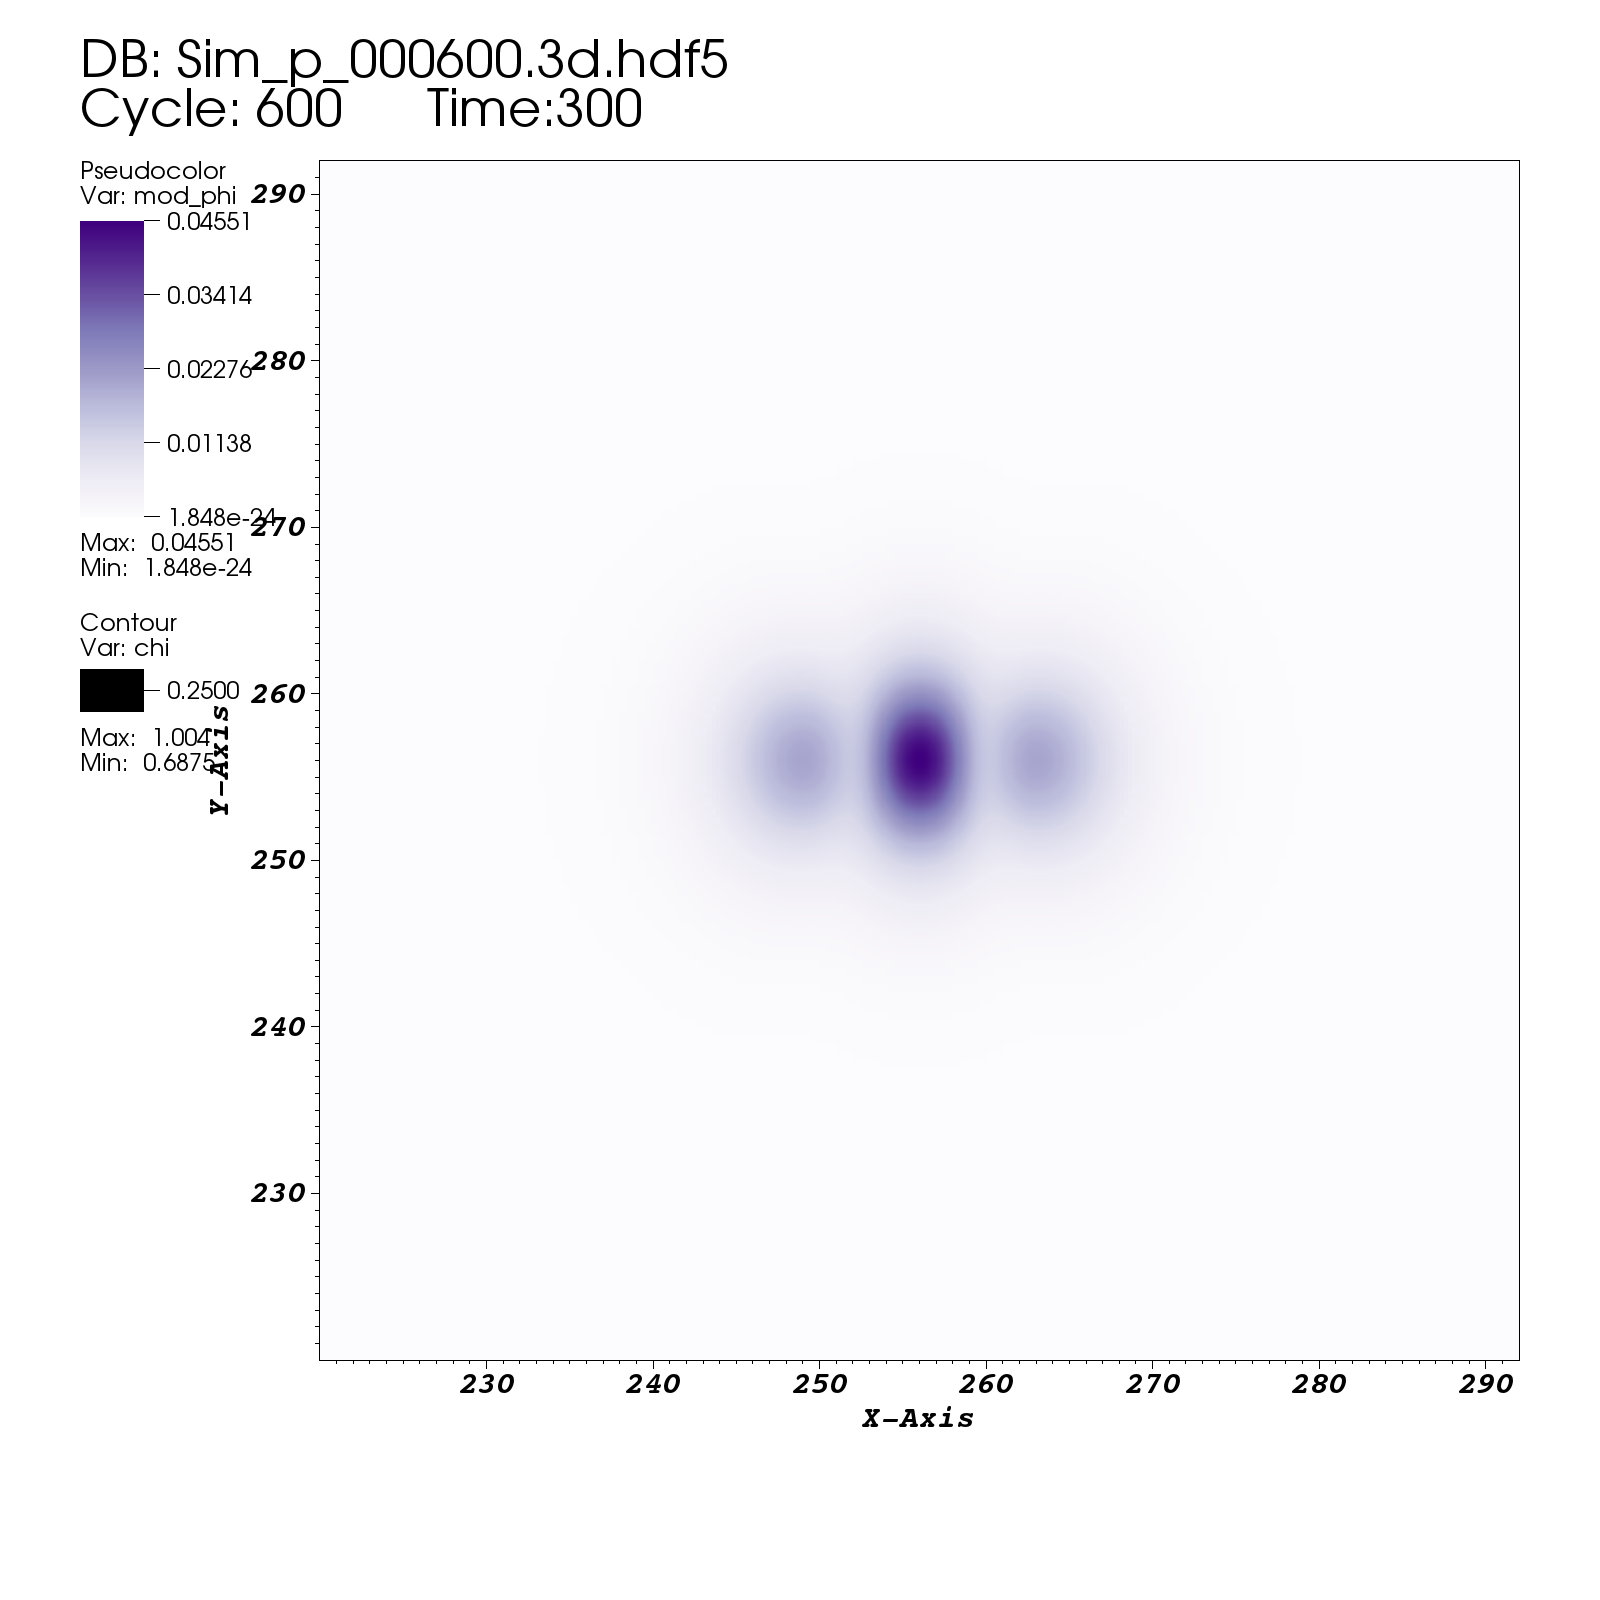
\includegraphics[width=0.50\textwidth]{modphi/headon_mod_phi0012.png}}
  \hspace{0 mm}
  \subfloat{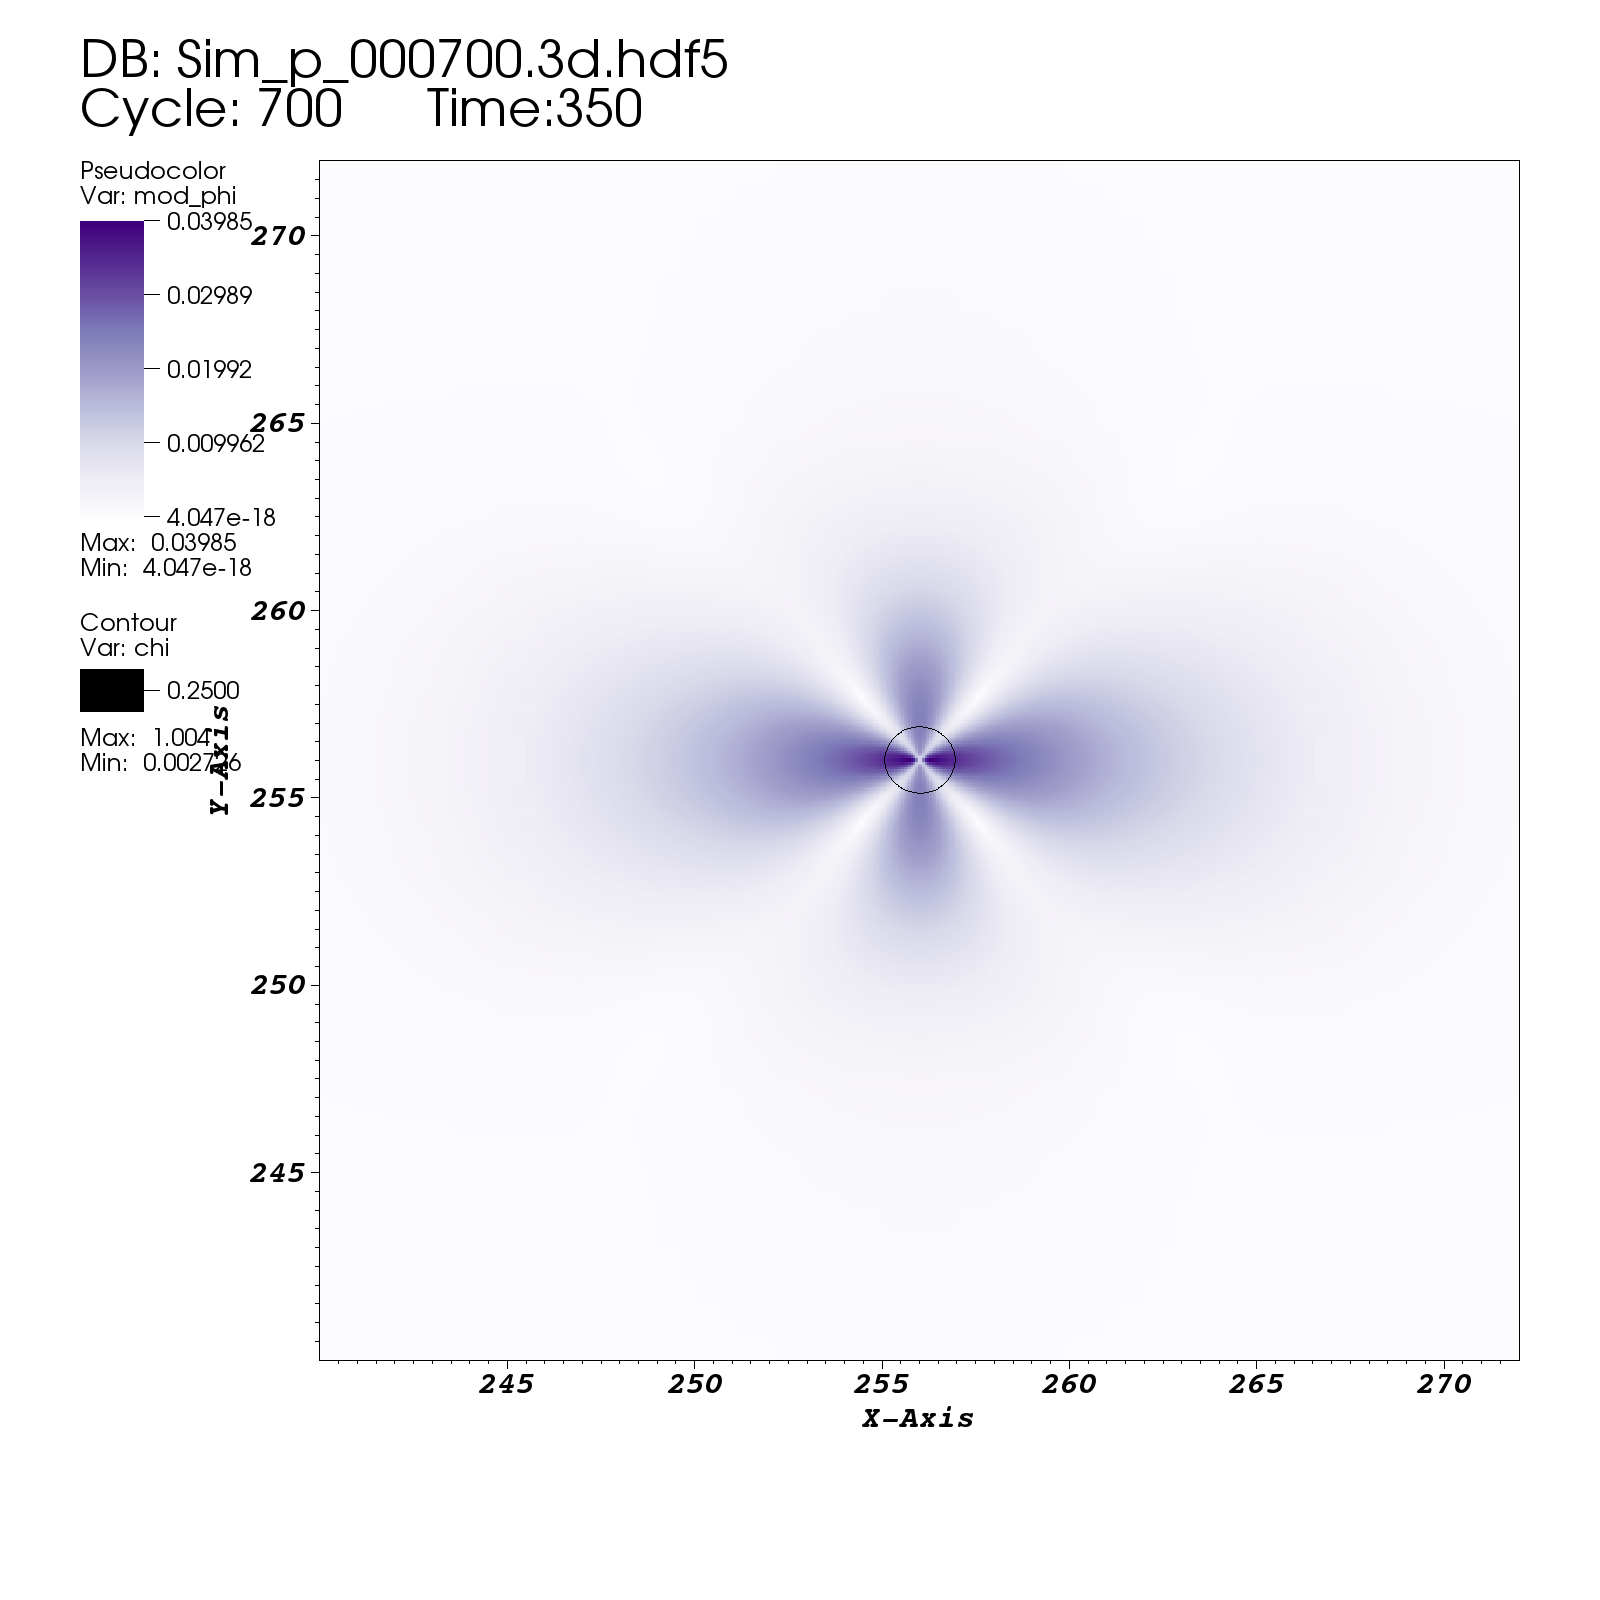
\includegraphics[width=0.50\textwidth]{modphi/headon_mod_phi0014.png}}\hfill
  \subfloat{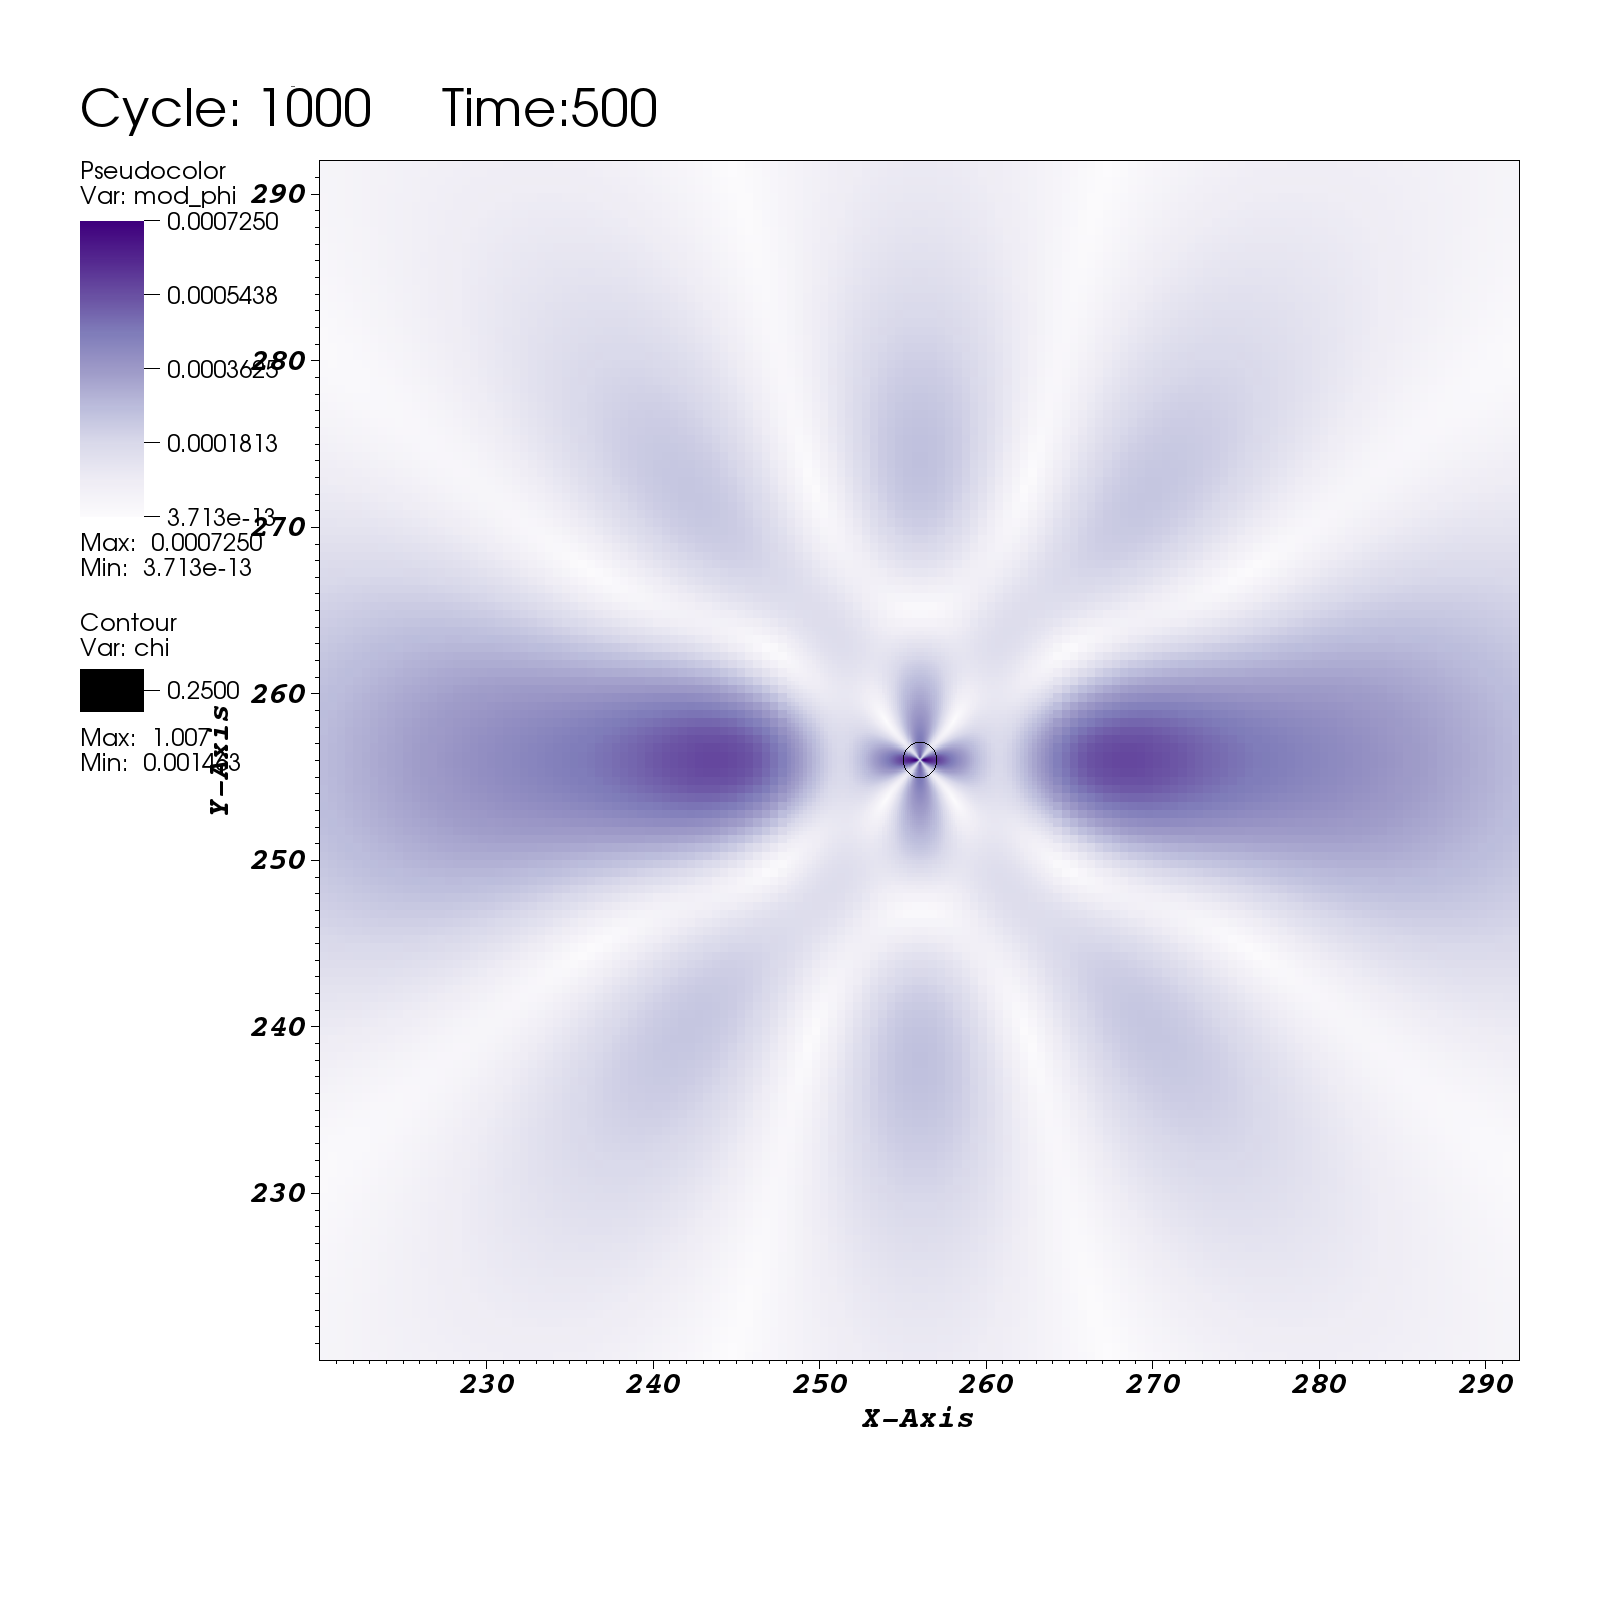
\includegraphics[width=0.50\textwidth]{modphi/headon_mod_phi0020.png}}
  \caption{Field plots of $|\vp|$ during evolution at four different times. Time $t=275~m^{-1}$ and $t=300~m^{-1}$ show snapshots momentarily before and after star collision. Time $t=350~m^{-1}$ shows the scalar field accreting into the recently formed black hole. Time $t= 500~m^{-1}$ shows the scalar field surrounding the black hole a little later; notably the amplitude is lower. Both the plots of $t=350~m^{-1}$ and $t=500~m^{-1}$ include a contour plot of $\chi=0.25$ acting as an approximate marker for the event horizon. The Newtonian estimate of collision time is $t= 287.6~m^{-1}$.}
  \label{boson:fig:ff7}
\end{figure}






\begin{figure}[h!]
\subfloat{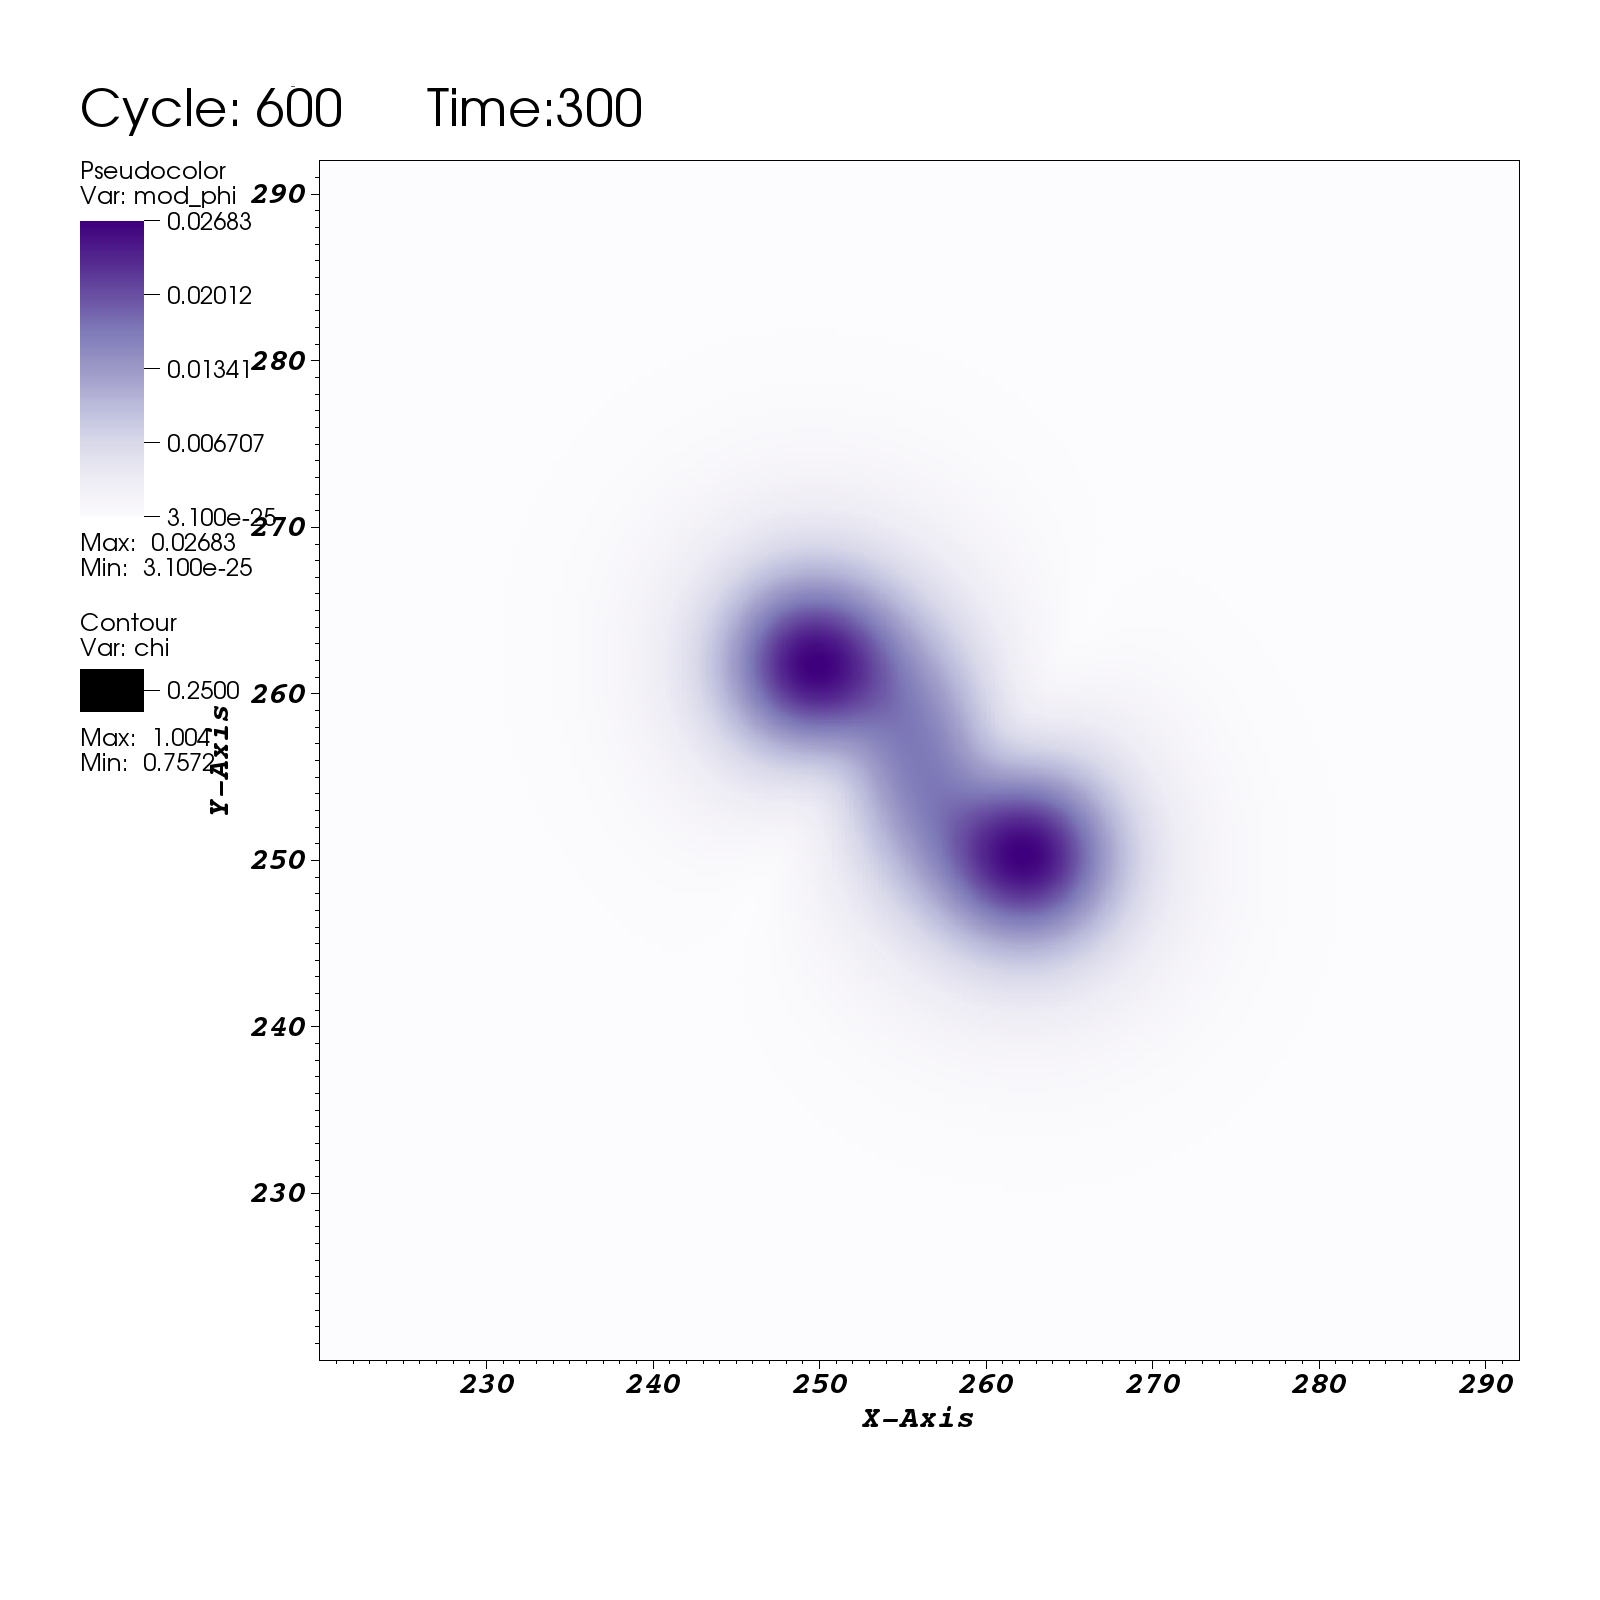
\includegraphics[width=0.5\textwidth]{modphi/graze_mod_phi0012.png}}\hfill
\subfloat{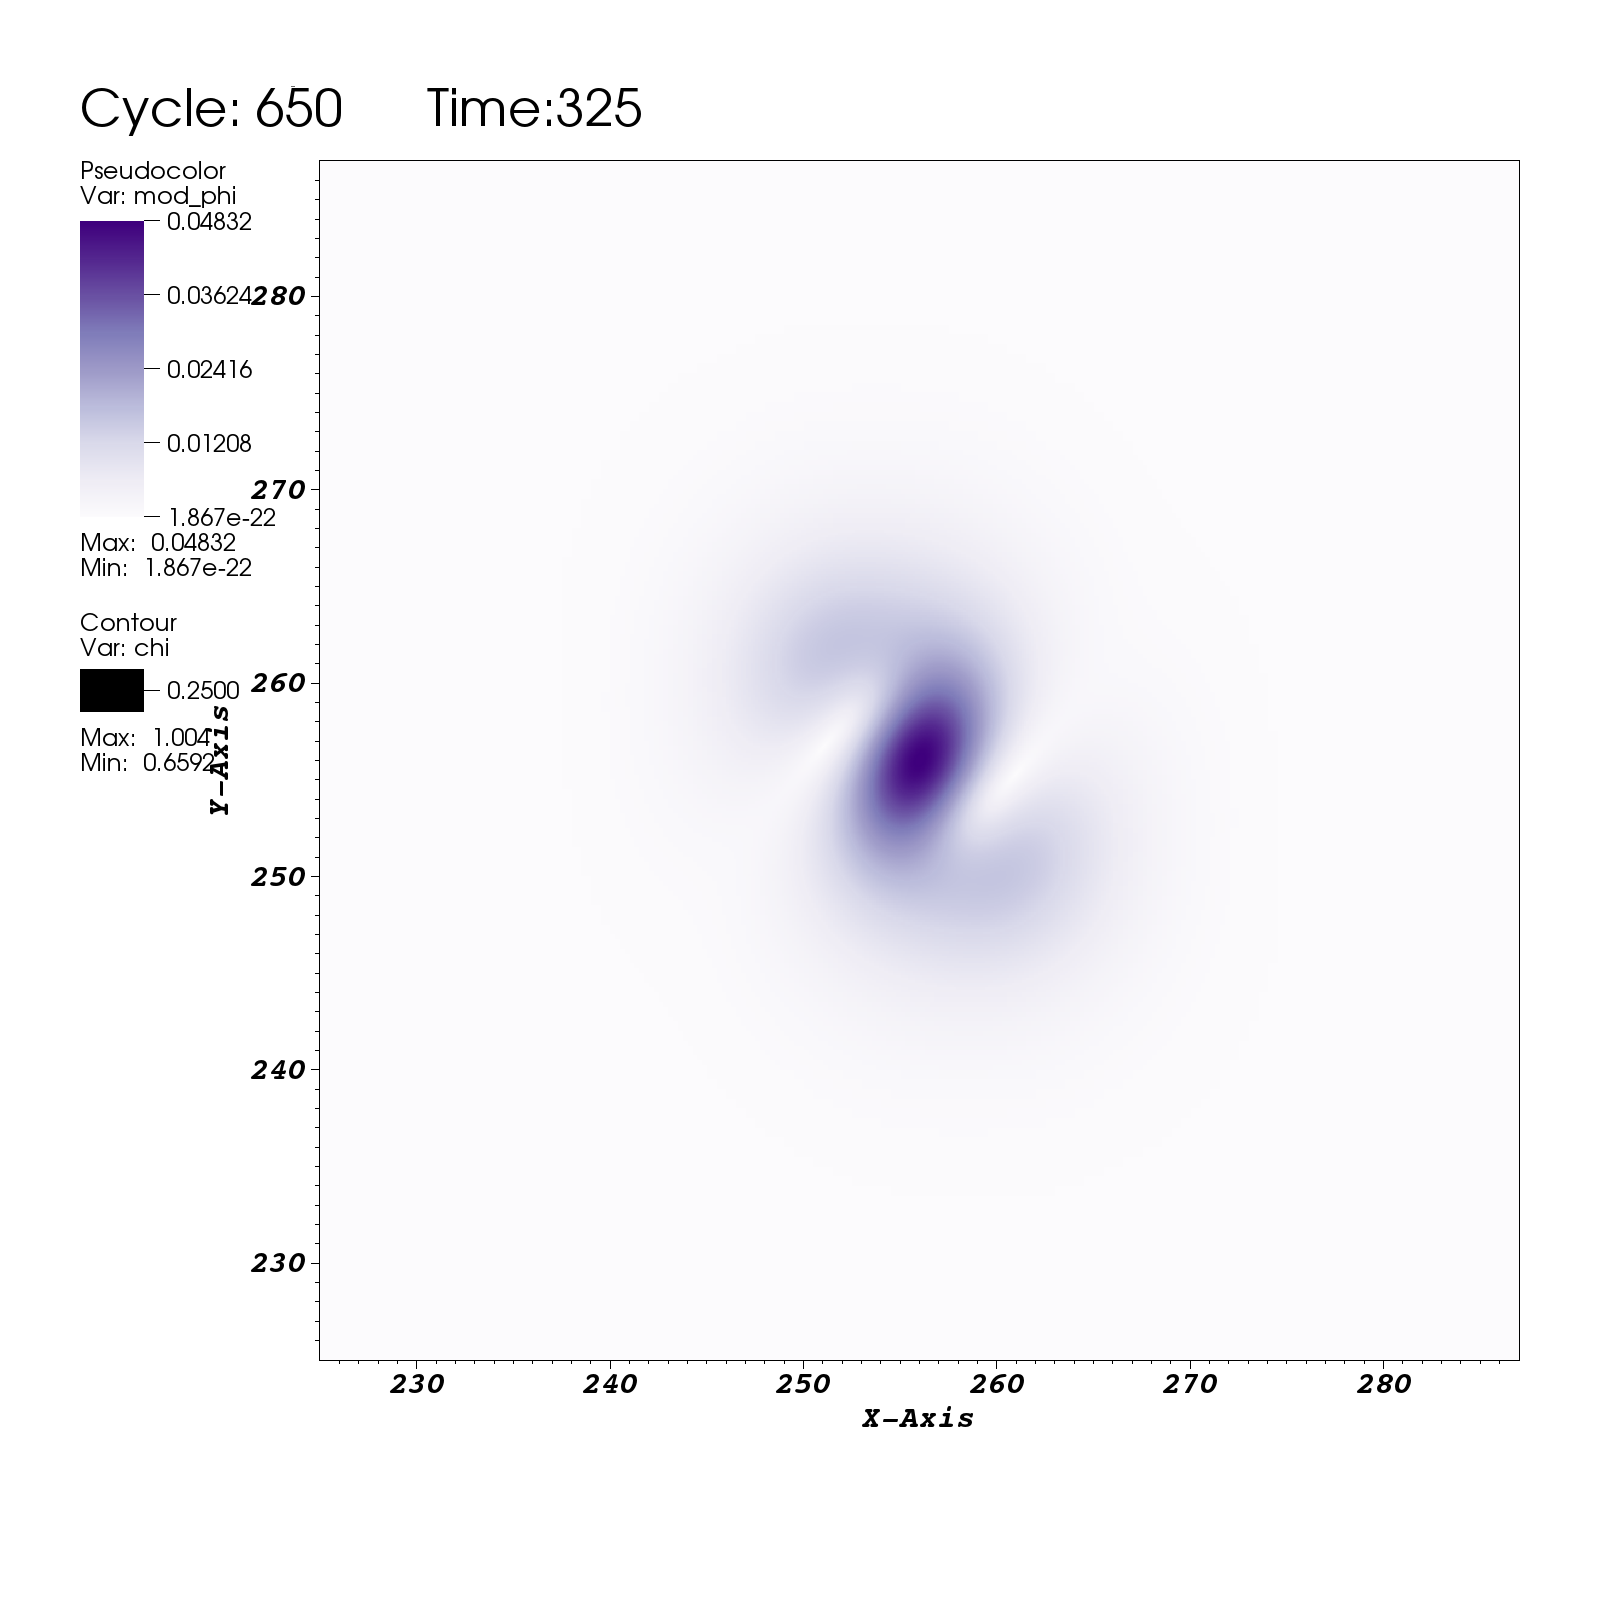
\includegraphics[width=0.5\textwidth]{modphi/graze_mod_phi0013.png}}
\hspace{0 mm}
\subfloat{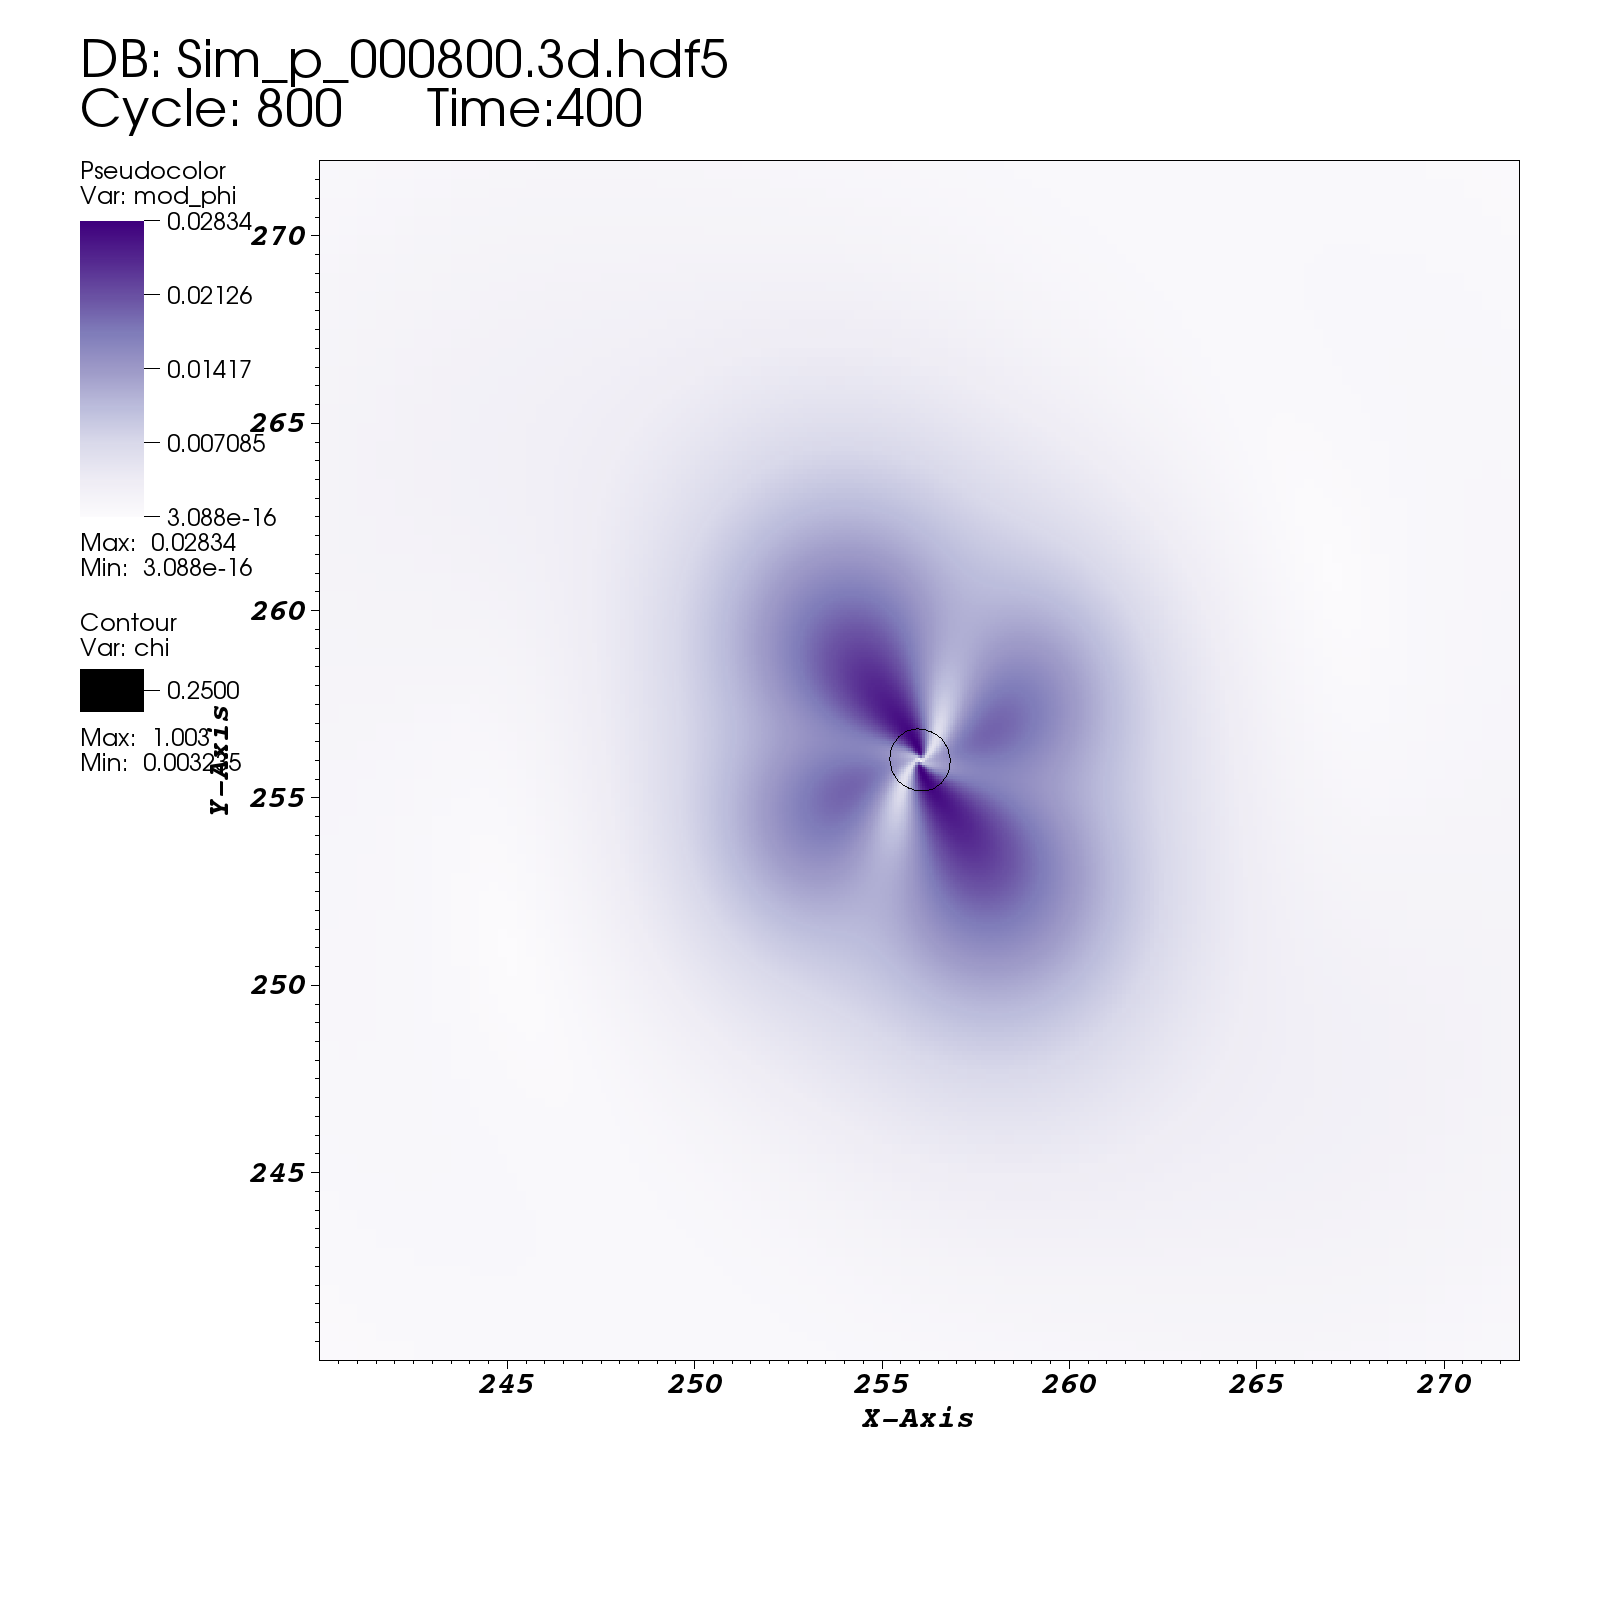
\includegraphics[width=0.5\textwidth]{modphi/graze_mod_phi0016.png}}\hfill
\subfloat{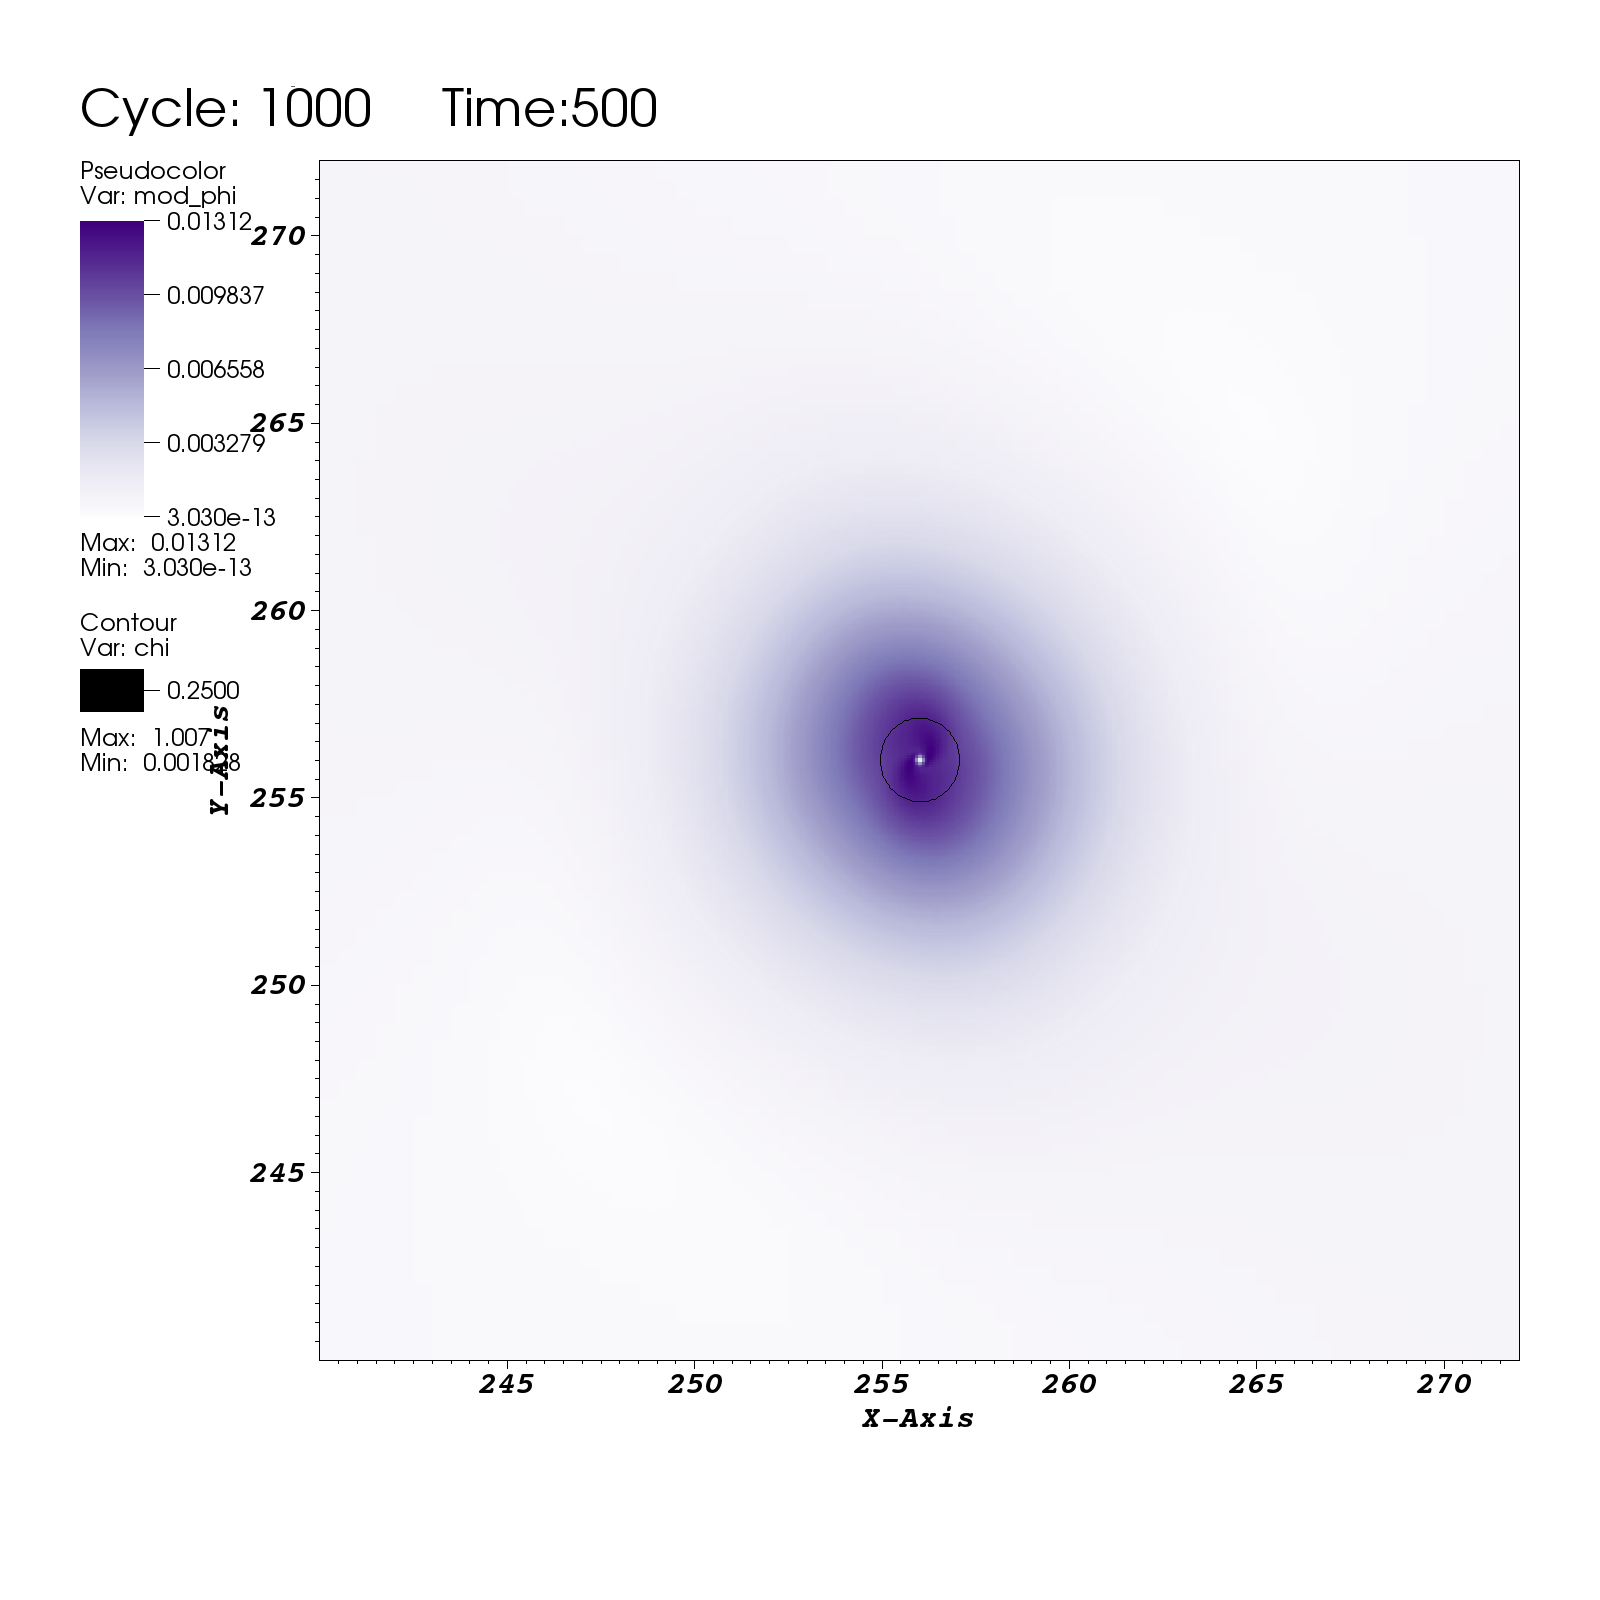
\includegraphics[width=0.5\textwidth]{modphi/graze_mod_phi0020.png}}
\caption{Field plots of $|\vp|$ during evolution at four different times for the grazing boson star collision. Time $t=300~m^{-1}$ and $t=325~m^{-1}$ show snapshots momentarily before and after the collision. The Newtonian estimate of collision time is $t= 315.8~m^{-1}$. Time $t=400~m^{-1}$ shows the scalar field accreting into the recently formed black hole. Time $t= 500~m^{-1}$ shows the scalar field surrounding the black hole a little later; here this is called a {\it toroidal wig}. Both the plots of $t=400~m^{-1}$ and $t=500~m^{-1}$ display a contour plot of $\chi=0.25$ acting as an approximate marker for the event horizon. }
\label{boson:fig:ff10}
\end{figure}



%BLACKHOLESBLACKHOLESBLACKHOLESBLACKHOLESBLACKHOLESBLACKHOLESBLACKHOLESBLACKHOLESBLACKHOLESBLACKHOLESBLACKHOLESBLACKHOLESBLACKHOLESBLACKHOLESBLACKHOLESBLACKHOLESBLACKHOLESBLACKHOLESBLACKHOLESBLACKHOLESBLACKHOLESBLACKHOLESBLACKHOLESBLACKHOLESBLACKHOLESBLACKHOLESBLACKHOLESBLACKHOLESBLACKHOLESBLACKHOLESBLACKHOLESBLACKHOLESBLACKHOLESBLACKHOLESBLACKHOLESBLACKHOLESBLACKHOLESBLACKHOLESBLACKHOLESBLACKHOLESBLACKHOLESBLACKHOLESBLACKHOLESBLACKHOLESBLACKHOLESBLACKHOLESBLACKHOLESBLACKHOLESBLACKHOLESBLACKHOLESBLACKHOLESBLACKHOLESBLACKHOLESBLACKHOLESBLACKHOLESBLACKHOLESBLACKHOLESBLACKHOLESBLACKHOLESBLACKHOLESBLACKHOLESBLACKHOLESBLACKHOLESBLACKHOLES


% \subsection{Collisions of Boson Stars with Black Holes} \label{grchombo:sec:bsbhcollisions}

% Here the headon and grazing collisions of a boson star with a black hole are presented. The superposition scheme is given in section \ref{grchombo:sec:superposition}. Similarly to the previous section on the collision of two identical stars, the star and black hole mass are identical, each with an ADM mass $M=0.532(7)$. The black hole and star are placed at positions $\pm\{40,0,0\}$ in the headon case and $\pm\{40,8,0\}$ in the grazing case and are boosted together with respective velocities $\mp\{0.1,0,0\}$ corresponding to a rapidity of $\psi=0.1003353$ (4 s.f.). The simulations have a physical domain size $L=512$ with $N=256$ gridpoints on AMR level zero, this gives a coarse grid resolution of $\Delta x = 2$. There are up to five extra AMR levels giving a finest grid resolution of $\Delta x = 16$.

% \subsubsection{Headon Collision}
%  \begin{figure}[h!]
%   \caption{Left: Maximum of $|\vp|$ during evolution, Right: Total integrated Noether charge $N$.}
%   \centering
%   \subfloat{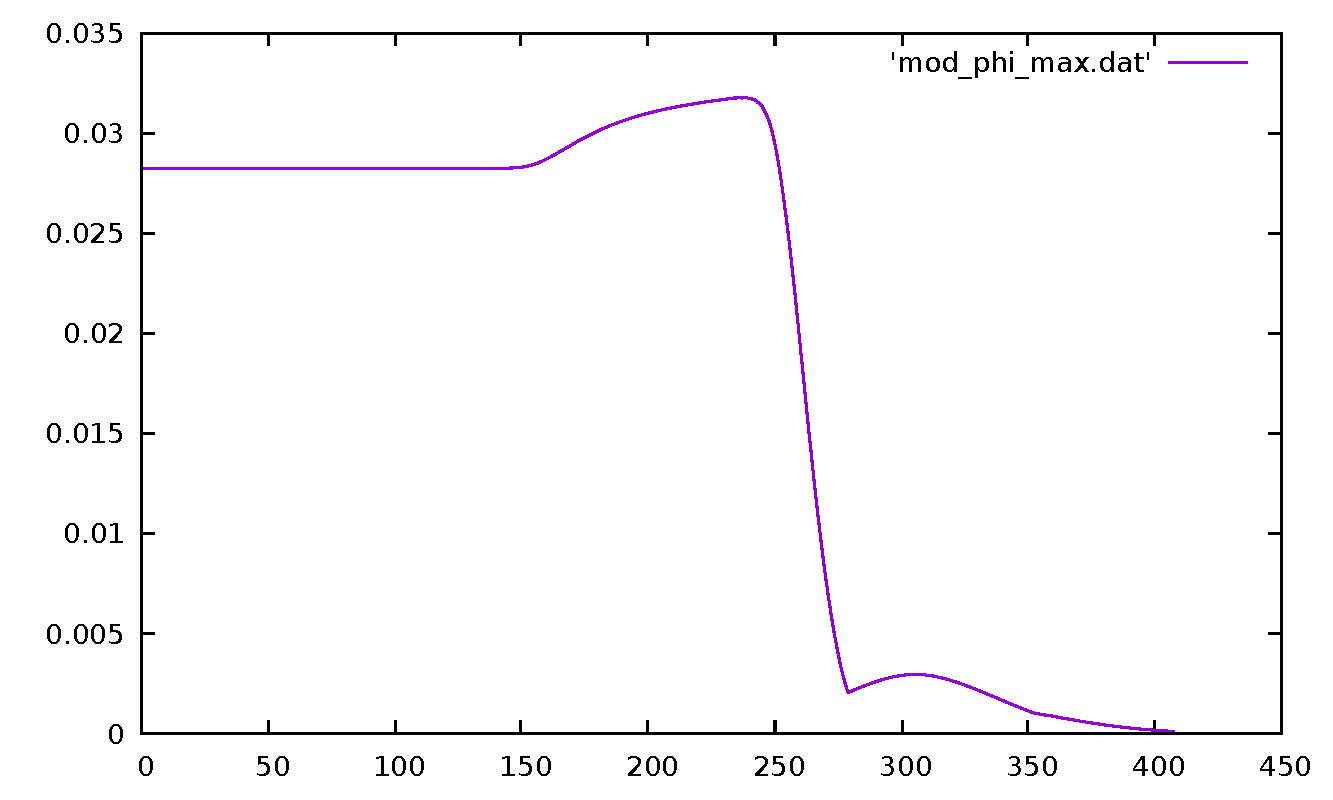
\includegraphics[width=0.5\textwidth]{data/headon_bhbs_modphi.pdf}\label{boson:fig:f12}}
%   \hfill
%   \subfloat{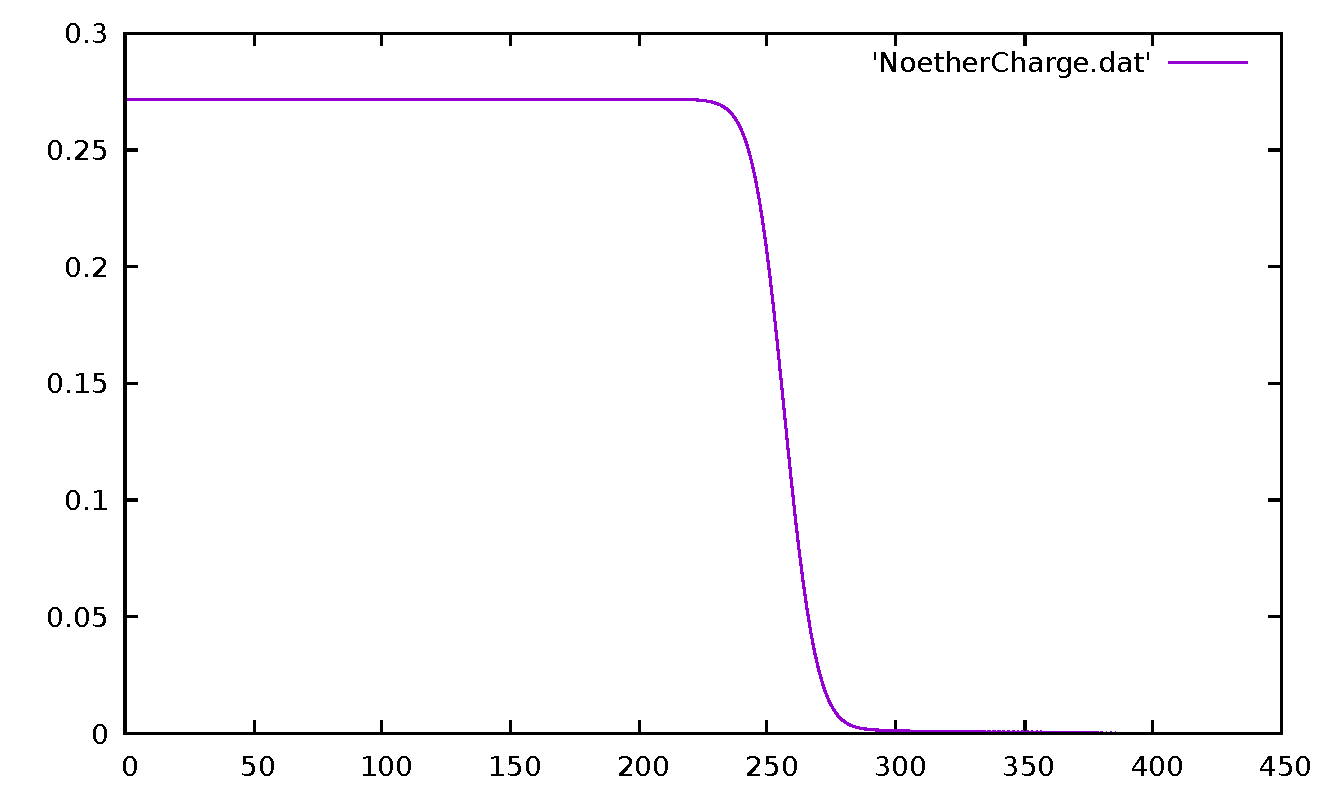
\includegraphics[width=0.5\textwidth]{data/headon_bhbs_n.pdf}\label{boson:fig:f13}}
% \end{figure}

% Figure (\ref{boson:fig:f7}) shows $|\vp|_{\rm max}$, the global maximum value of $|\vp|$, and the total Noether charge as a function of time for the headon collision. At time $t\approx 289 \cdot m$, $|\vp|_{\rm max}$ rapidly increases; a black hole is then formed. At time $t\approx 327 \cdot m$, $|\vp|_{\rm max}$ there is a temporal maximum in $|\vp|_{\rm max}$ as the resolution limit of the simulation is reached and the scalar field is damped away by the Kreiss-Oliger dissipation mentioned in section \ref{grchombo:sec:grchombo}. This damping can also be seen in the Noether charge plot, at a time of $t \approx 326 \cdot m$, where the total charge that should remain constant falls. The lack of sufficient resolution inside the black hole is not disasterous to the external simulation fortunately; the erorrs accumulated are trapped inside the event horizon.

% The gravitational wave extraction at radius $r=140 \cdot m$ is given in figure \ref{boson:fig:f9}. A spin-weighted spherical harmonic decomposition of the Newman-Penrose scalar $\Psi_4$ [REF] has been done and the $m,l = 2,0$ and $m,l = 2,2$ modes are plotted.

% \begin{figure}[h!]
%   \caption{Left: Maximum of $|\vp|$ during evolution, Right: Total integrated Noether charge $N$.}
%   \centering
%   \subfloat{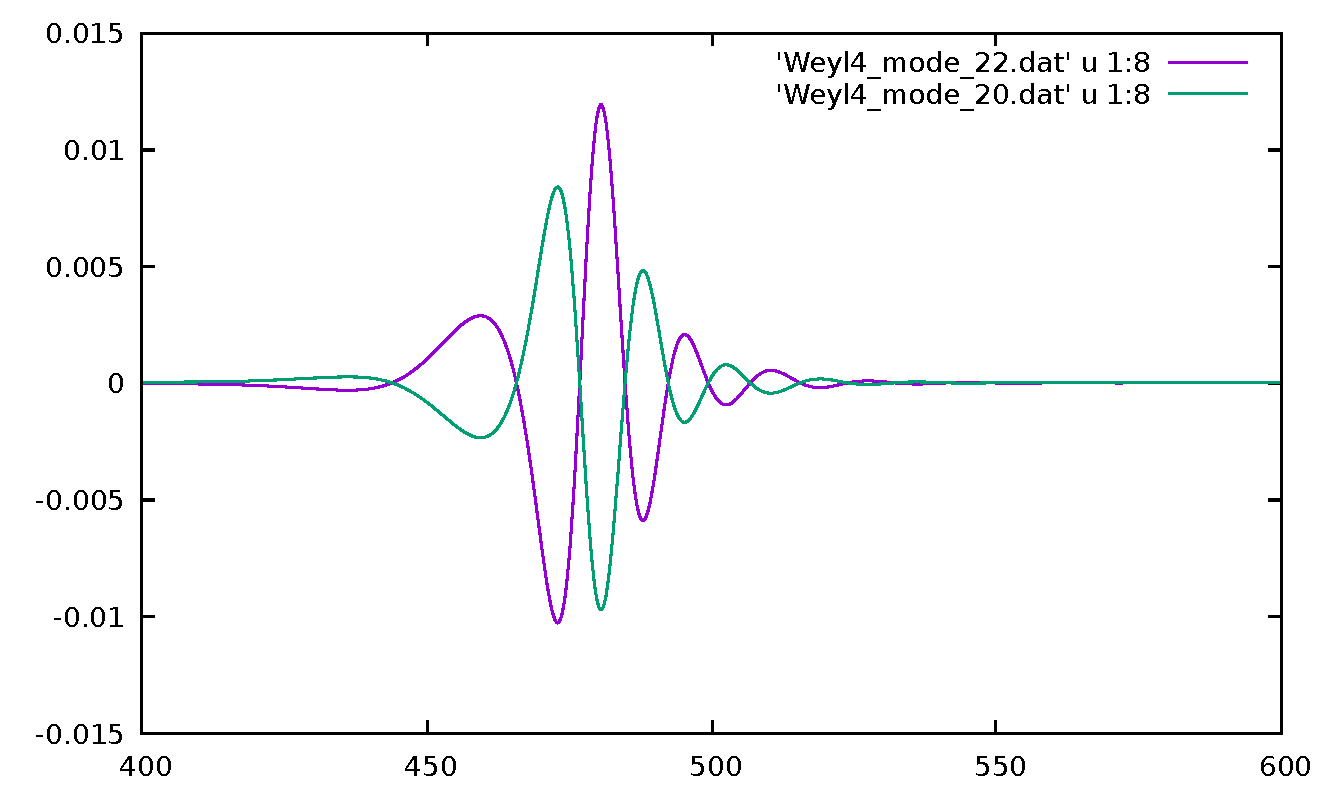
\includegraphics[width=0.5\textwidth]{data/headon_weyl22.pdf}\label{boson:fig:f14}}
% \end{figure}



% The dynamics of the two boson stars are shown in Fig.~(\ref{boson:fig:ff7}) plotting the scalar field modulus $|\vp|$ on the $x,y$ plane. The stars collide at at time $275\cdot m < t < 300 \cdot m$ and soon after an overdensity of scalar field forms collapsing to a black hole. This black hole subsequently accretes the surrouding scalar field; Fig.~(\ref{boson:fig:f7}) shows that the total Noether charge rapidly decays to zero as it falls into the black hole and is dissipated due to finite resolution effects. MAYBE DONT PUT THIS TWICE?

% as can be seen from the remnannt moving in (cvia coordinates) the simaultion is not in the rest frame.







%  \begin{figure}[h!]
%   \caption{Field plots of $|\vp|$ during evolution at four different times. Time $t=200 \cdot m$ and $t=250 \cdot m$ show snapshots momentarily before and after the collision. Time $t=300 \cdot m$ shows the scalar field accreting into the black hole and time $t= 400 \cdot m$ shows the scalar field surrounding the black hole a little later; noteably the amplitude is lower. All plots have a contour plot of $\chi=0.25$ acting as a very approximate marker for the event horizon. The Newtonian estimate of collision time is $t= 287.6 \cdot m$.}
%   \subfloat{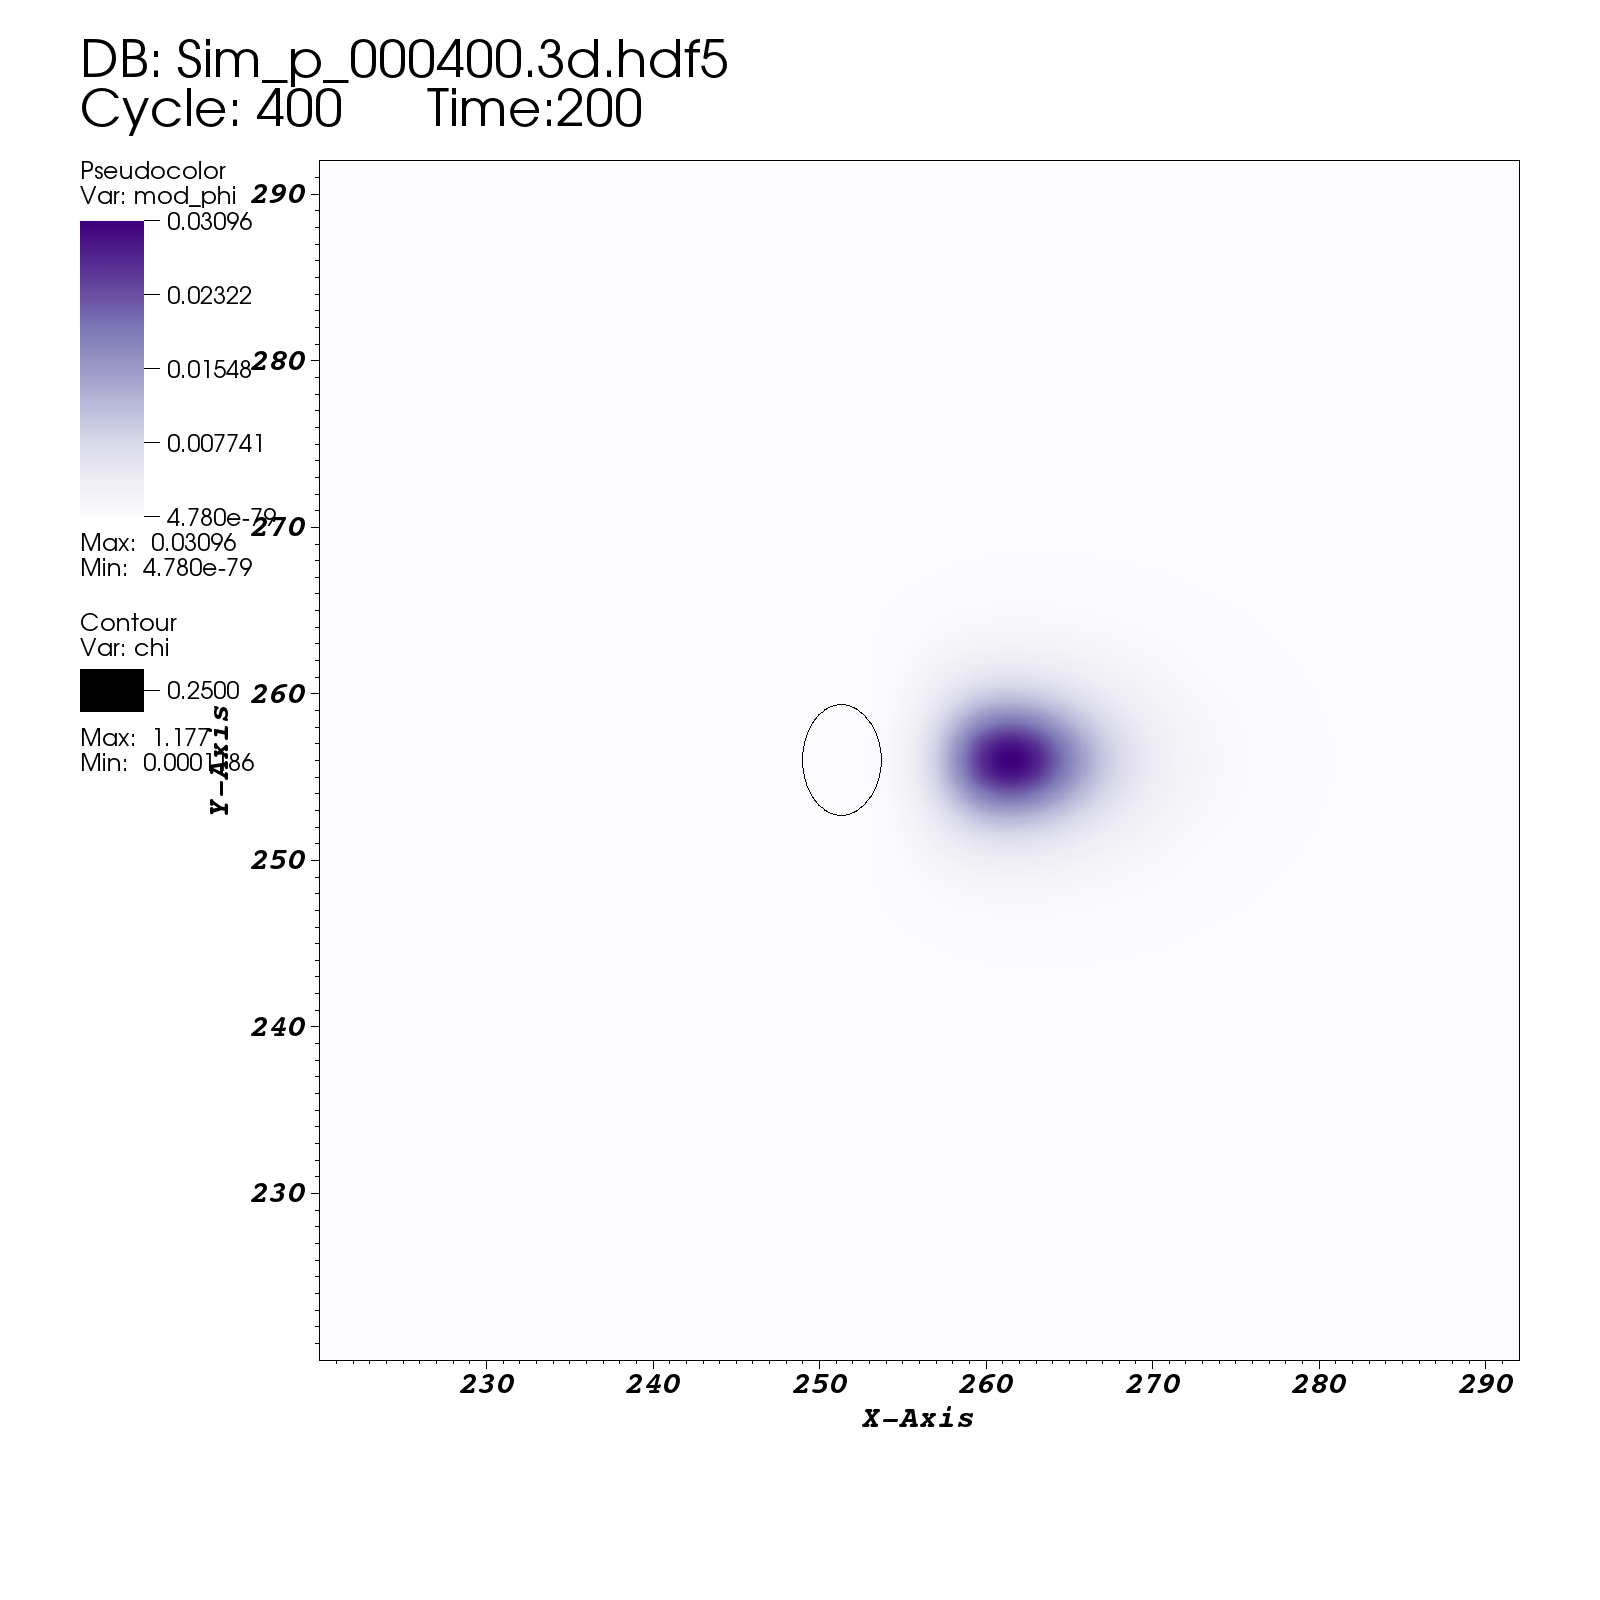
\includegraphics[width=0.45\textwidth]{modphi/headon_bhbs_mod_phi0008.png}\label{boson:fig:ff12}}
%   \subfloat{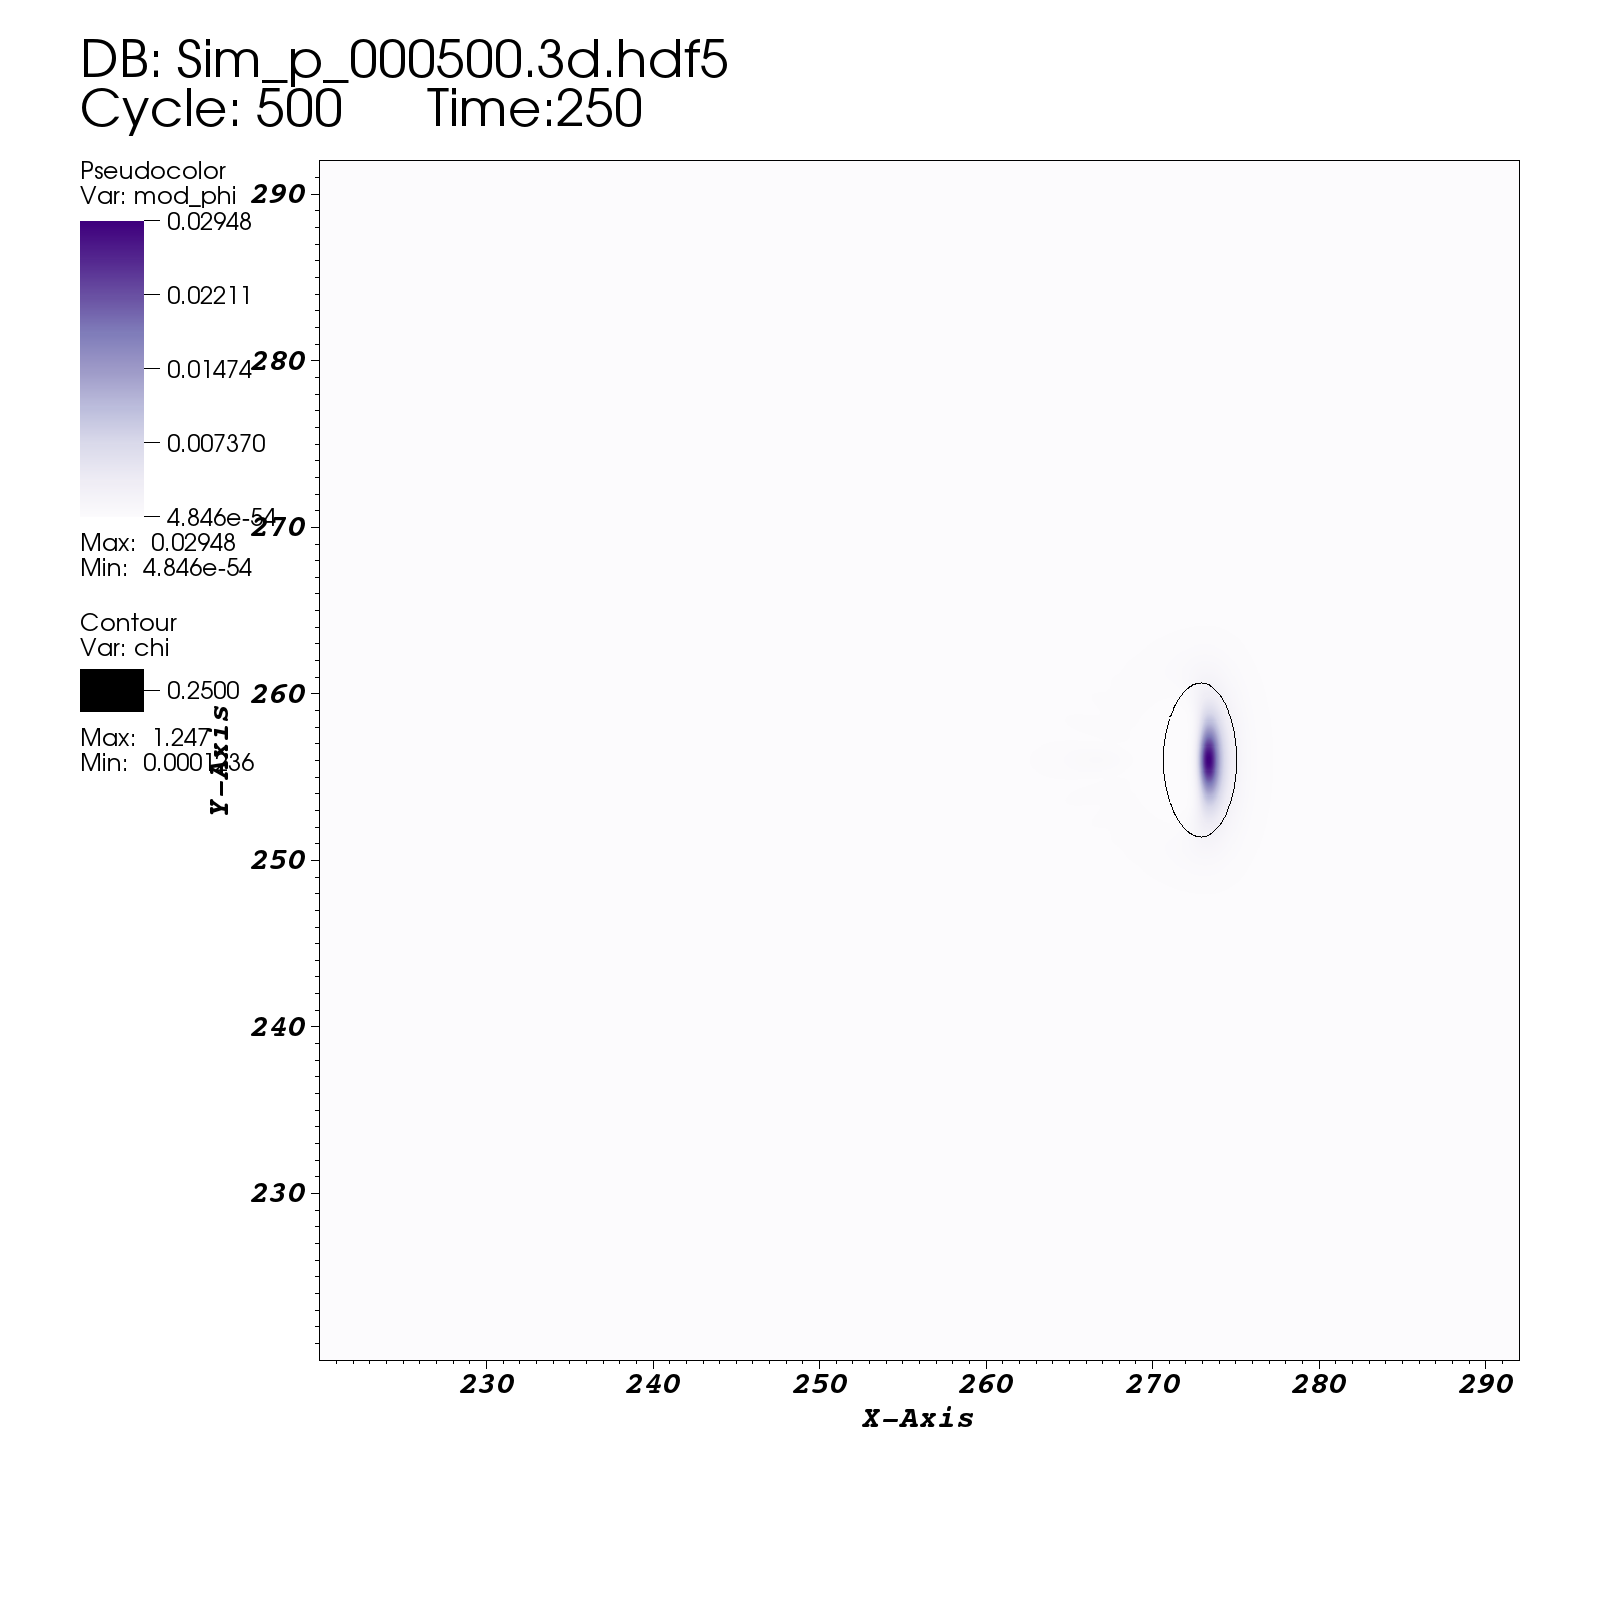
\includegraphics[width=0.45\textwidth]{modphi/headon_bhbs_mod_phi0010.png}}
%   \hfill
%   \subfloat{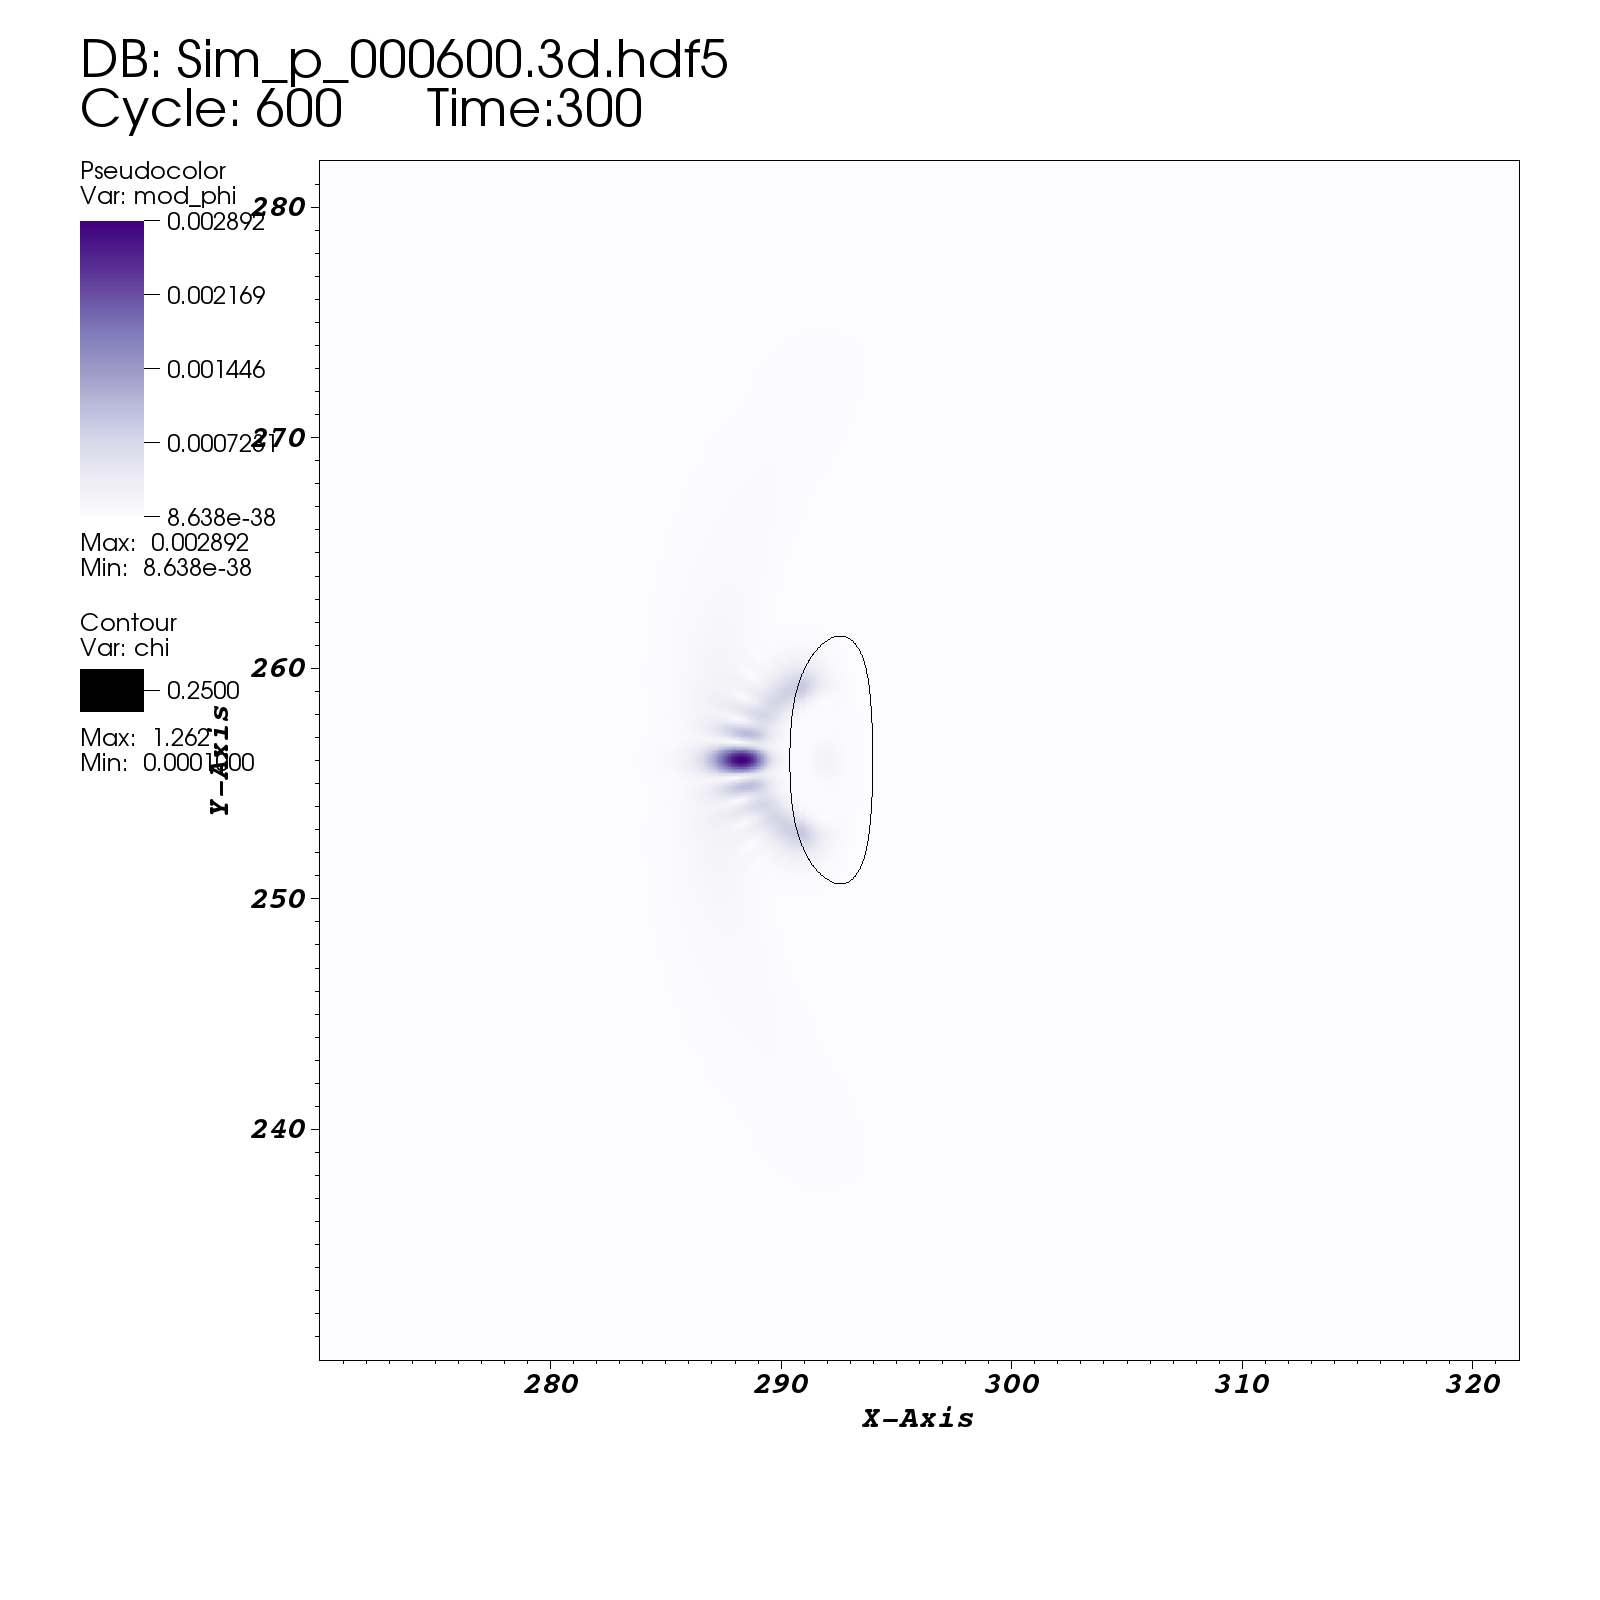
\includegraphics[width=0.45\textwidth]{modphi/headon_bhbs_mod_phi0012.png}}
%   \subfloat{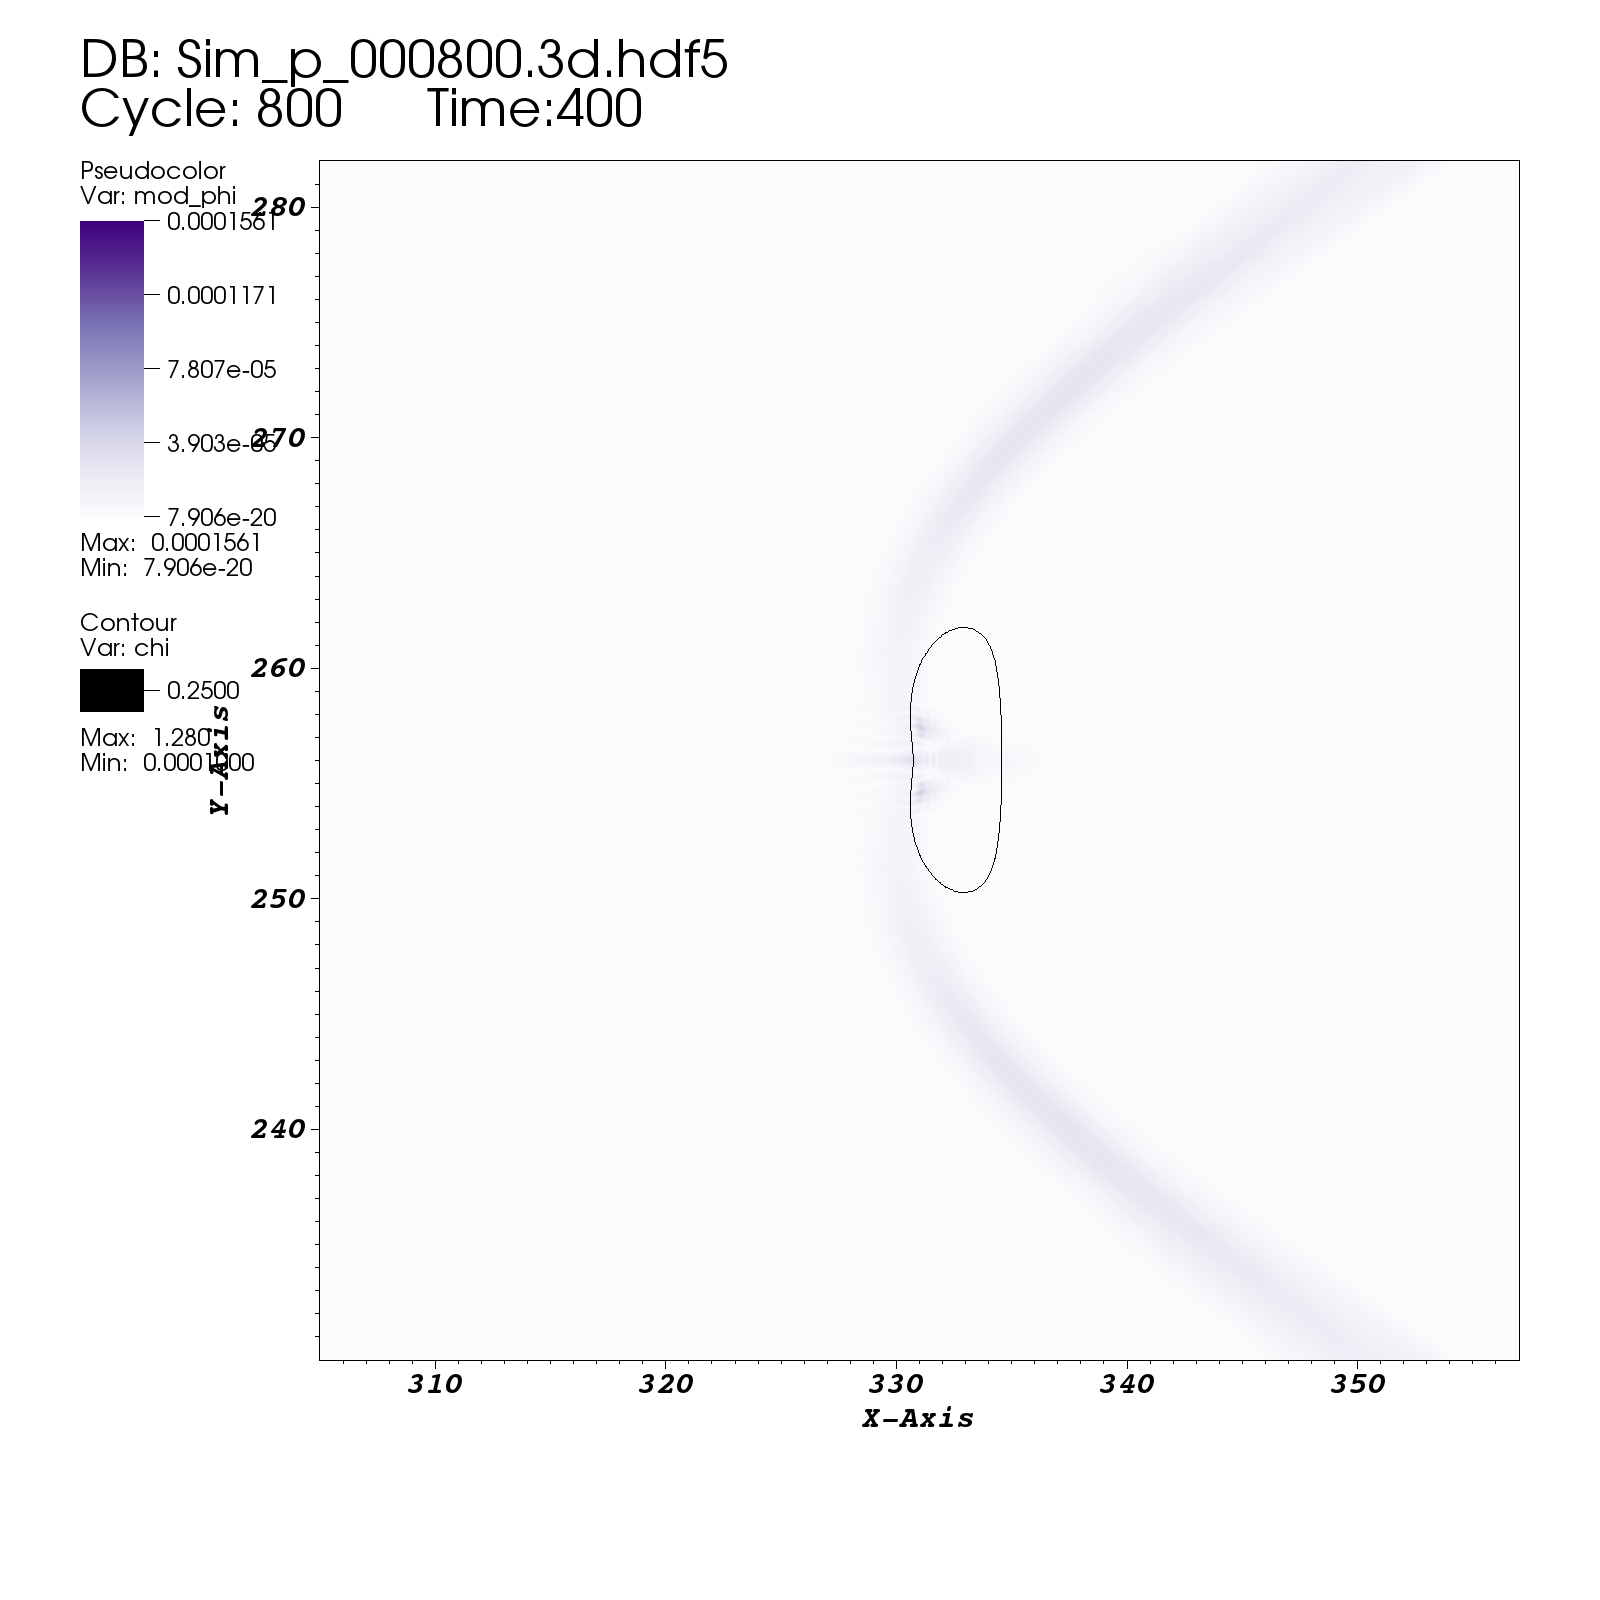
\includegraphics[width=0.45\textwidth]{modphi/headon_bhbs_mod_phi0016.png}}
% \end{figure}




% \subsubsection{Grazing Collision}
%  \begin{figure}[h!]
%   \caption{Left: Maximum of $|\vp|$ during evolution, Right: Total integrated Noether charge $N$.}
%   \centering
%   \subfloat{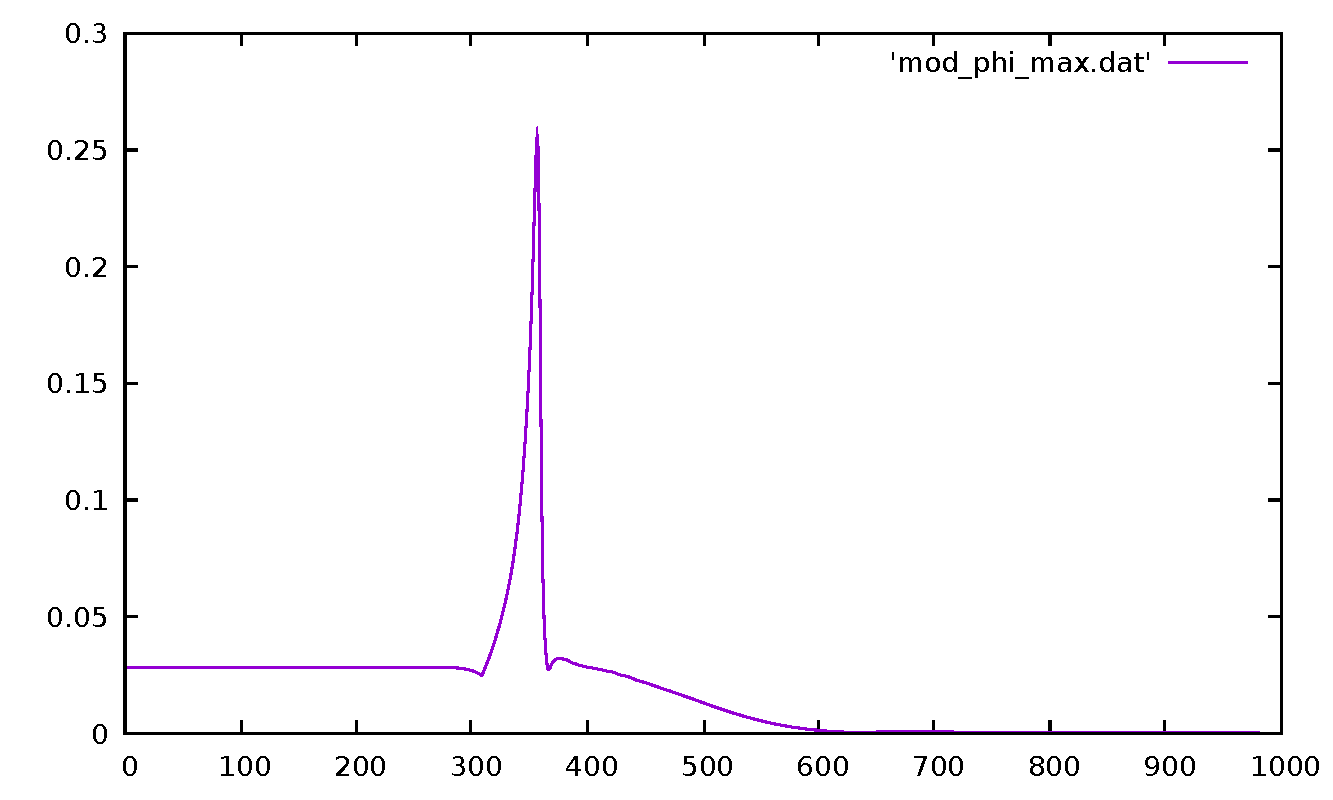
\includegraphics[width=0.5\textwidth]{data/graze_modphi.pdf}\label{boson:fig:f15}}
%   \hfill
%   \subfloat{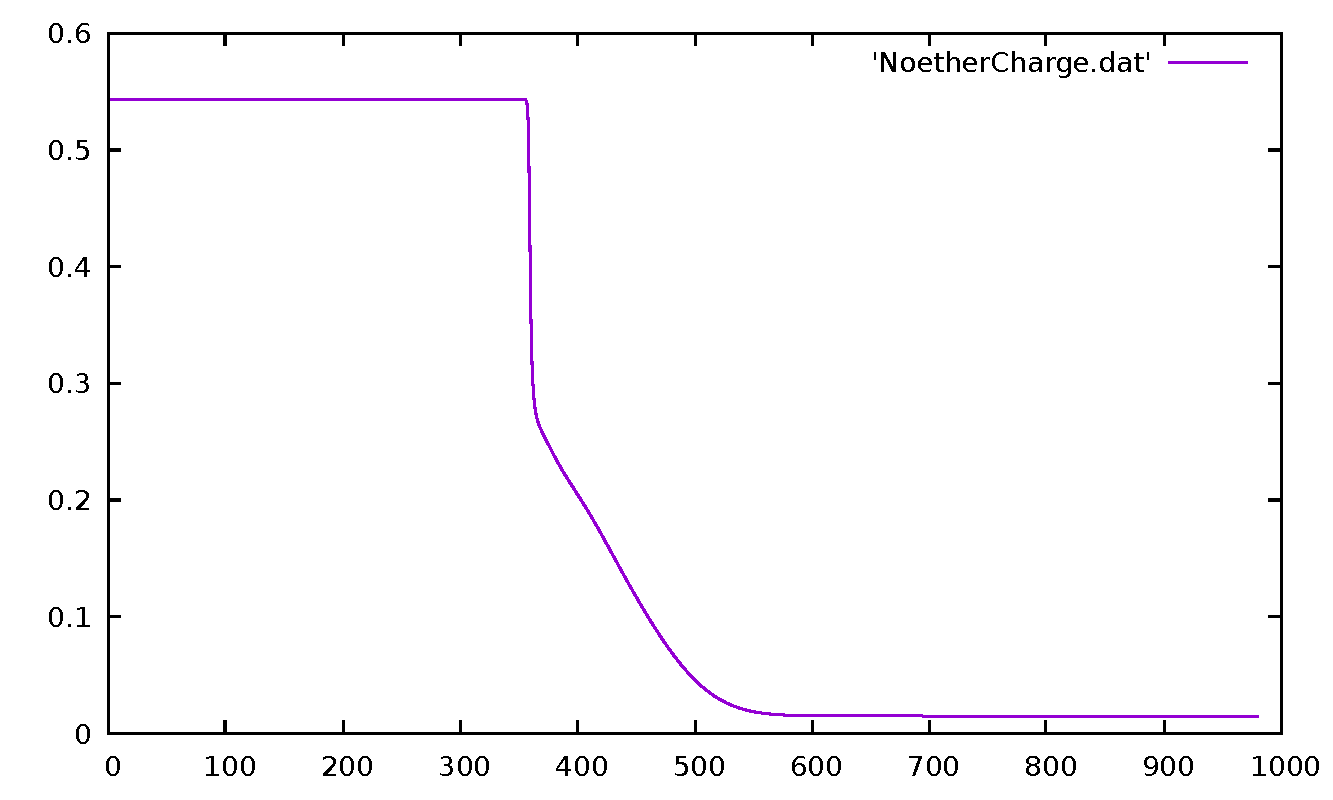
\includegraphics[width=0.5\textwidth]{data/graze_N.pdf}\label{boson:fig:f16}}
% \end{figure}

% Figure (\ref{boson:fig:f7}) shows $|\vp|_{\rm max}$, the global maximum value of $|\vp|$, and the total Noether charge as a function of time for the headon collision. At time $t\approx 289 \cdot m$, $|\vp|_{\rm max}$ rapidly increases; a black hole is then formed. At time $t\approx 327 \cdot m$, $|\vp|_{\rm max}$ there is a temporal maximum in $|\vp|_{\rm max}$ as the resolution limit of the simulation is reached and the scalar field is damped away by the Kreiss-Oliger dissipation mentioned in section \ref{grchombo:sec:grchombo}. This damping can also be seen in the Noether charge plot, at a time of $t \approx 326 \cdot m$, where the total charge that should remain constant falls. The lack of sufficient resolution inside the black hole is not disasterous to the external simulation fortunately; the erorrs accumulated are trapped inside the event horizon.

% The gravitational wave extraction at radius $r=140 \cdot m$ is given in figure \ref{boson:fig:f9}. A spin-weighted spherical harmonic decomposition of the Newman-Penrose scalar $\Psi_4$ [REF] has been done and the $m,l = 2,0$ and $m,l = 2,2$ modes are plotted.


% \begin{figure}[h!]
%   \caption{Left: Maximum of $|\vp|$ during evolution, Right: Total integrated Noether charge $N$.}
%   \centering
%   \subfloat{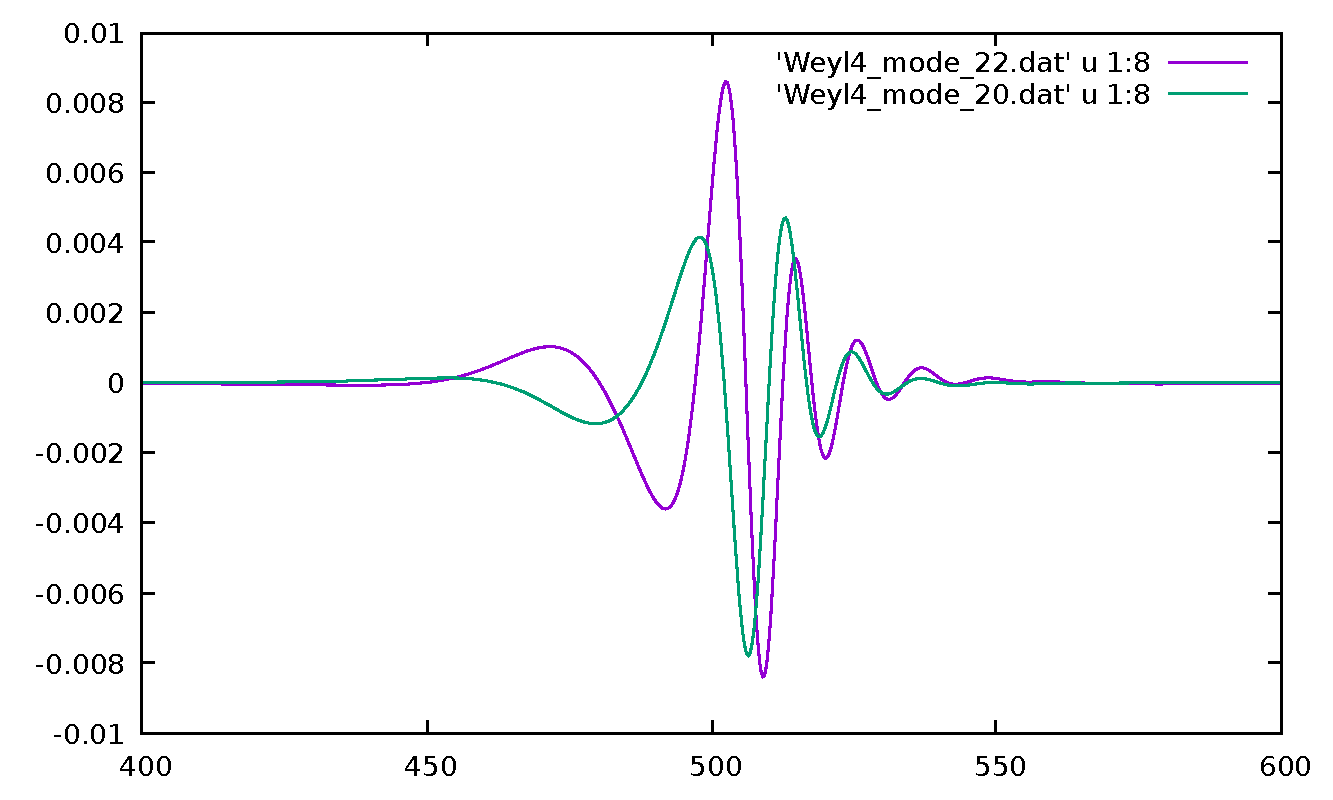
\includegraphics[width=0.5\textwidth]{data/graze_weyl22.pdf}\label{boson:fig:f17}}
% \end{figure}

% The dynamics of the two boson stars are shown in Fig.~(\ref{boson:fig:ff7}) plotting the scalar field modulus $|\vp|$ on the $x,y$ plane. The stars collide at at time $275\cdot m < t < 300 \cdot m$ and soon after an overdensity of scalar field forms collapsing to a black hole. This black hole subsequently accretes the surrouding scalar field; Fig.~(\ref{boson:fig:f7}) shows that the total Noether charge rapidly decays to zero as it falls into the black hole and is dissipated due to finite resolution effects. MAYBE DONT PUT THIS TWICE?



%  \begin{figure}[h!]
%   \caption{Left: Maximum of $|\vp|$ during evolution, Right: Total integrated Noether charge $N$.}
%   \subfloat{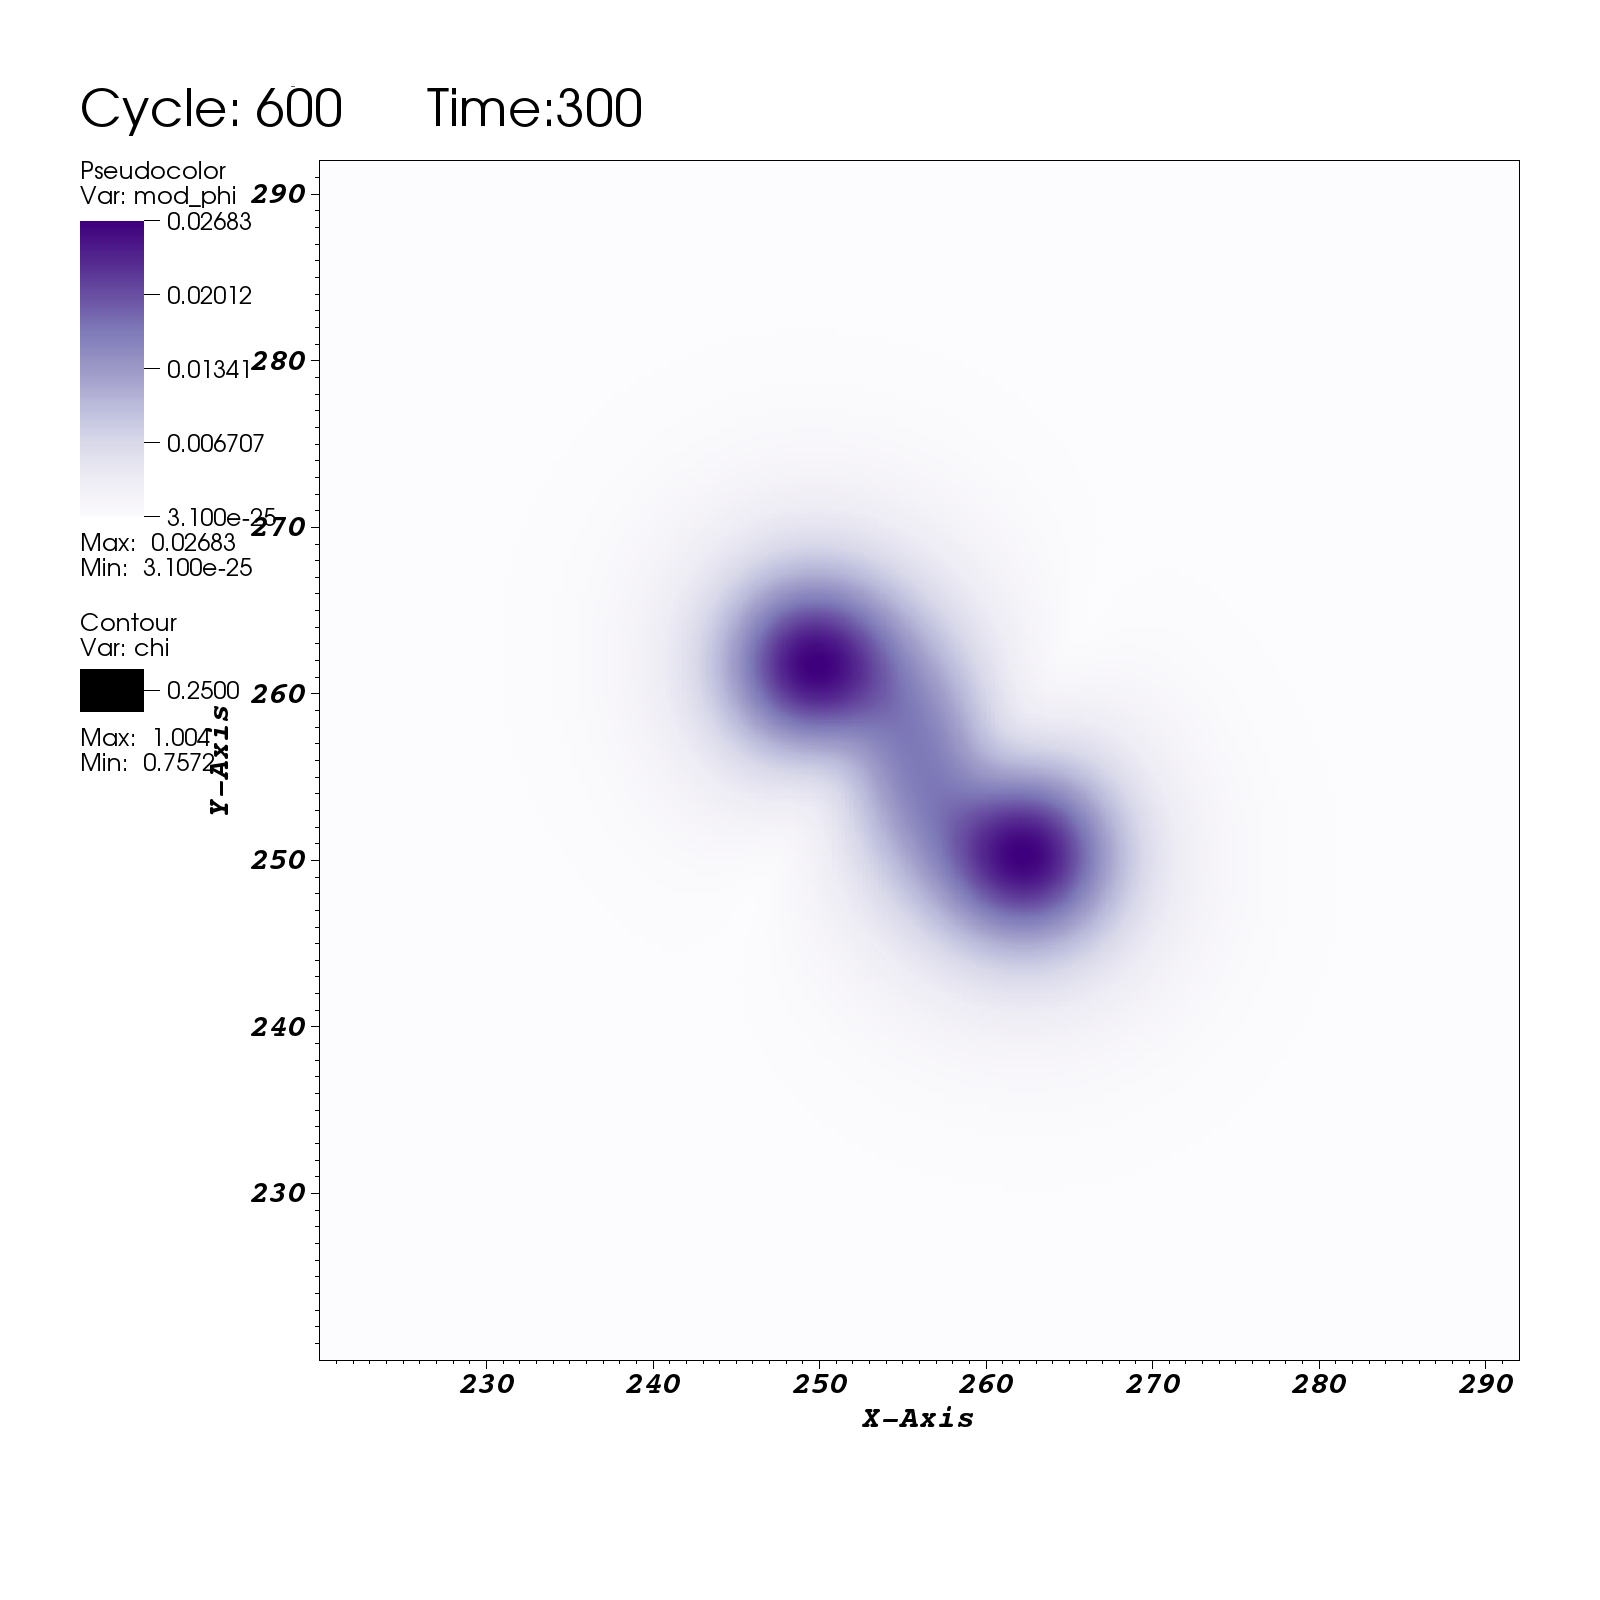
\includegraphics[width=0.45\textwidth]{modphi/graze_mod_phi0012.png}\label{boson:fig:ff15}}
%   \subfloat{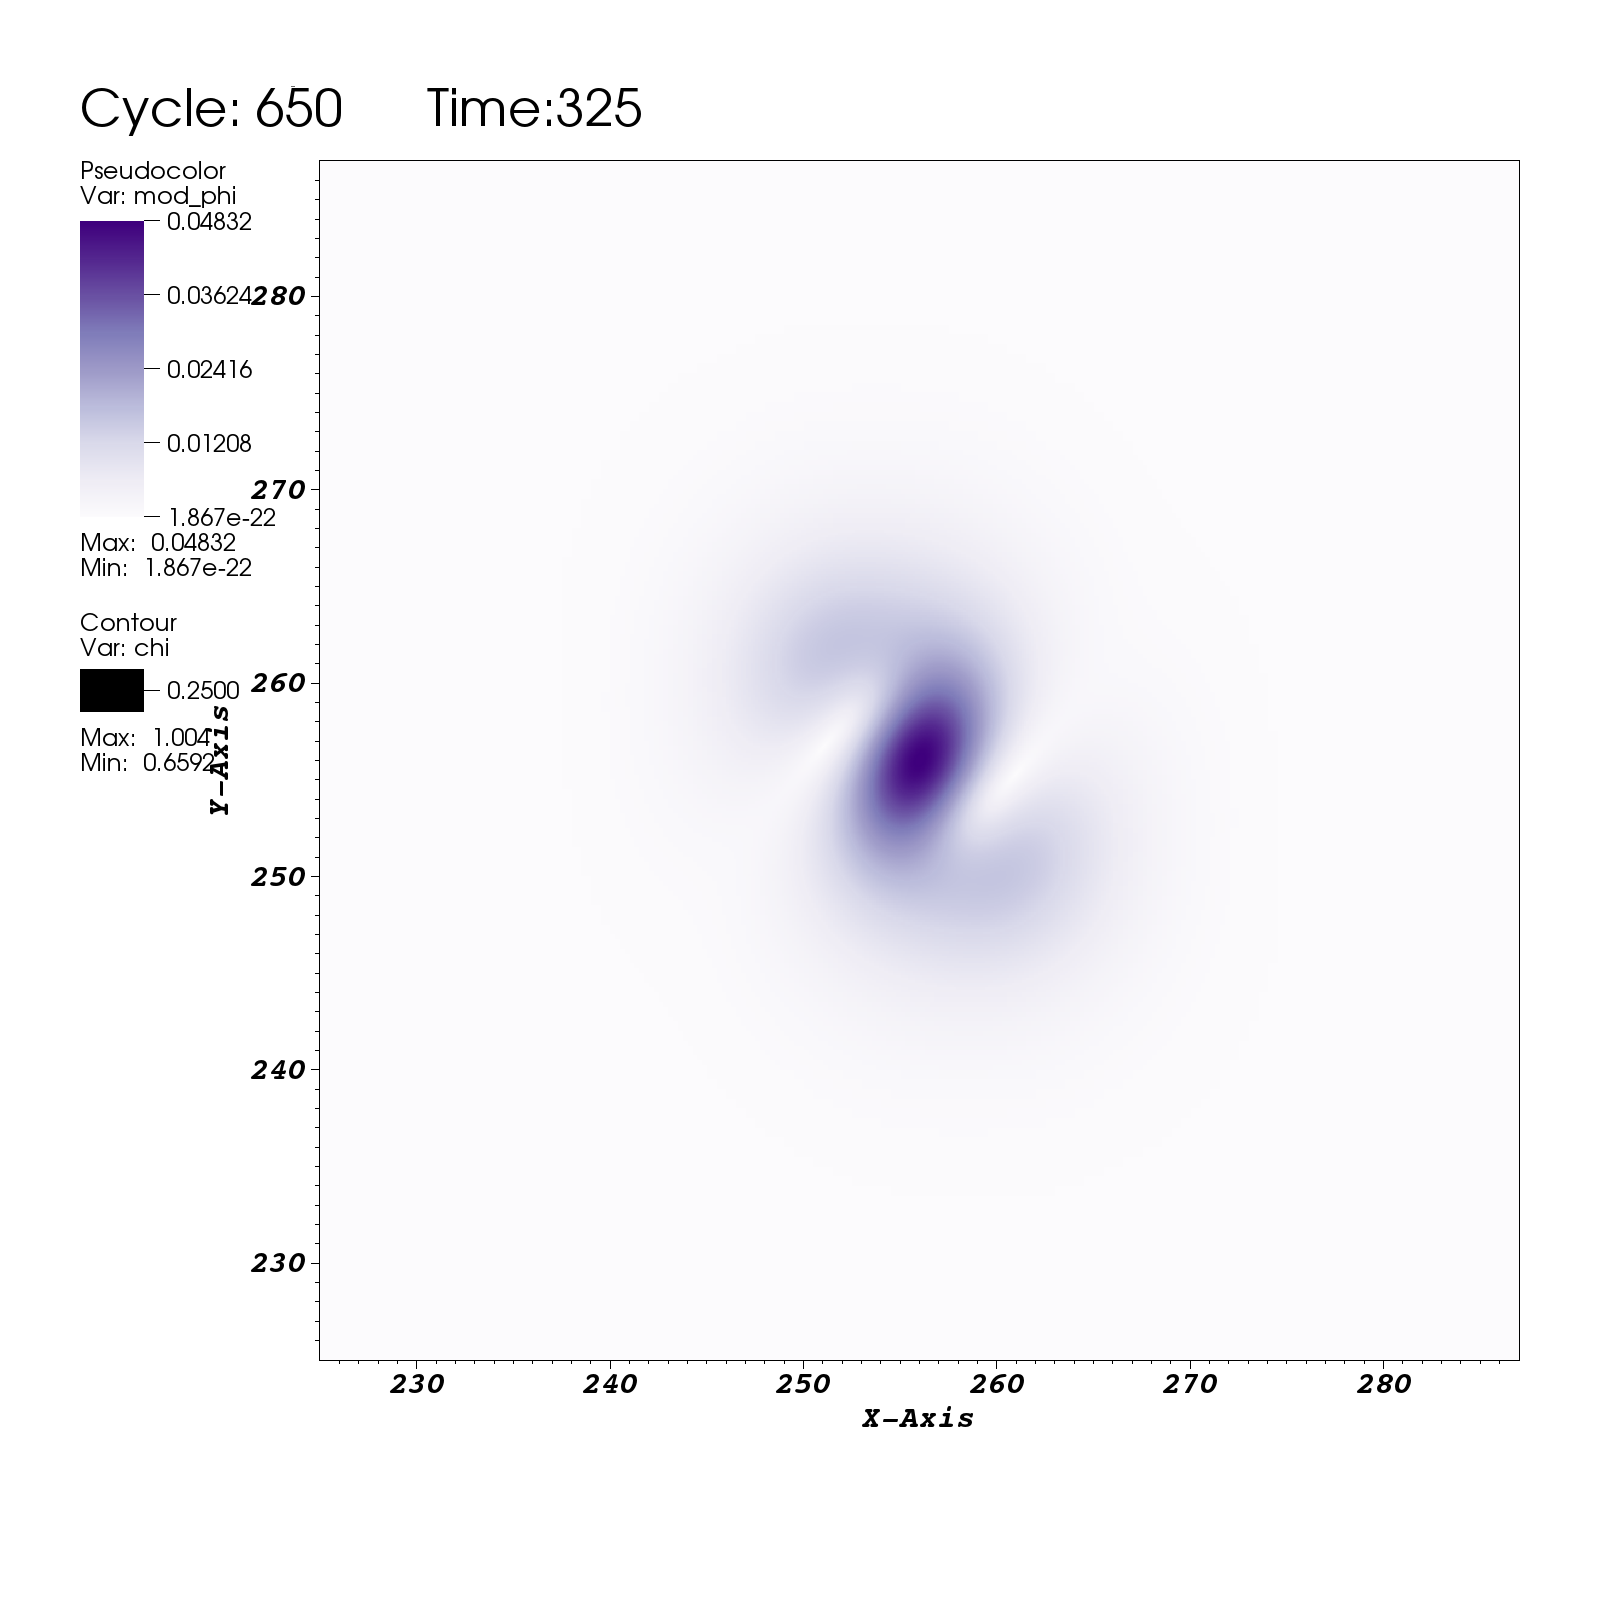
\includegraphics[width=0.45\textwidth]{modphi/graze_mod_phi0013.png}}
%   \hfill
%   \subfloat{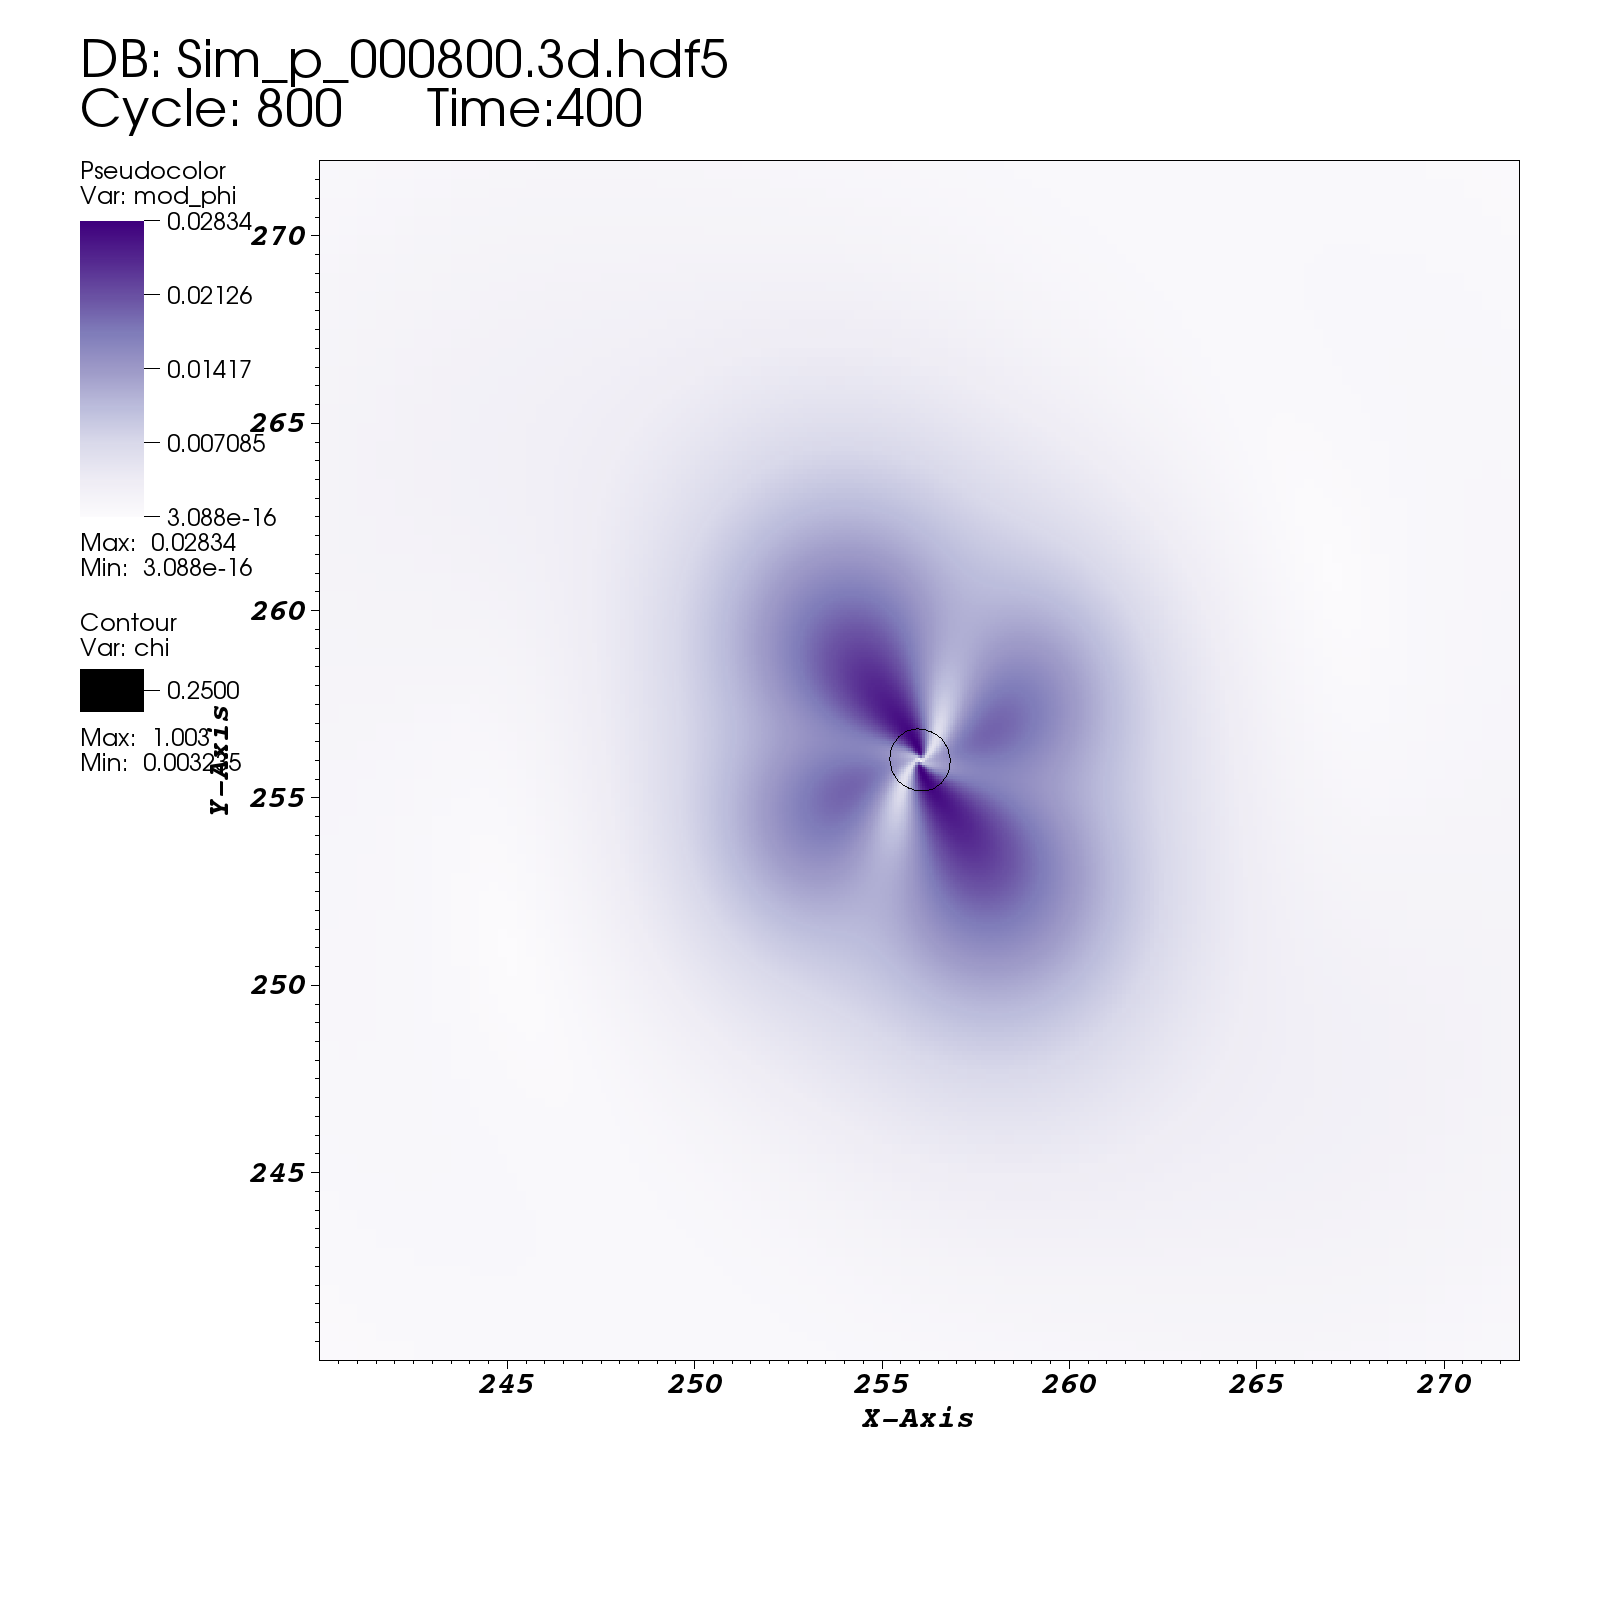
\includegraphics[width=0.45\textwidth]{modphi/graze_mod_phi0016.png}}
%   \subfloat{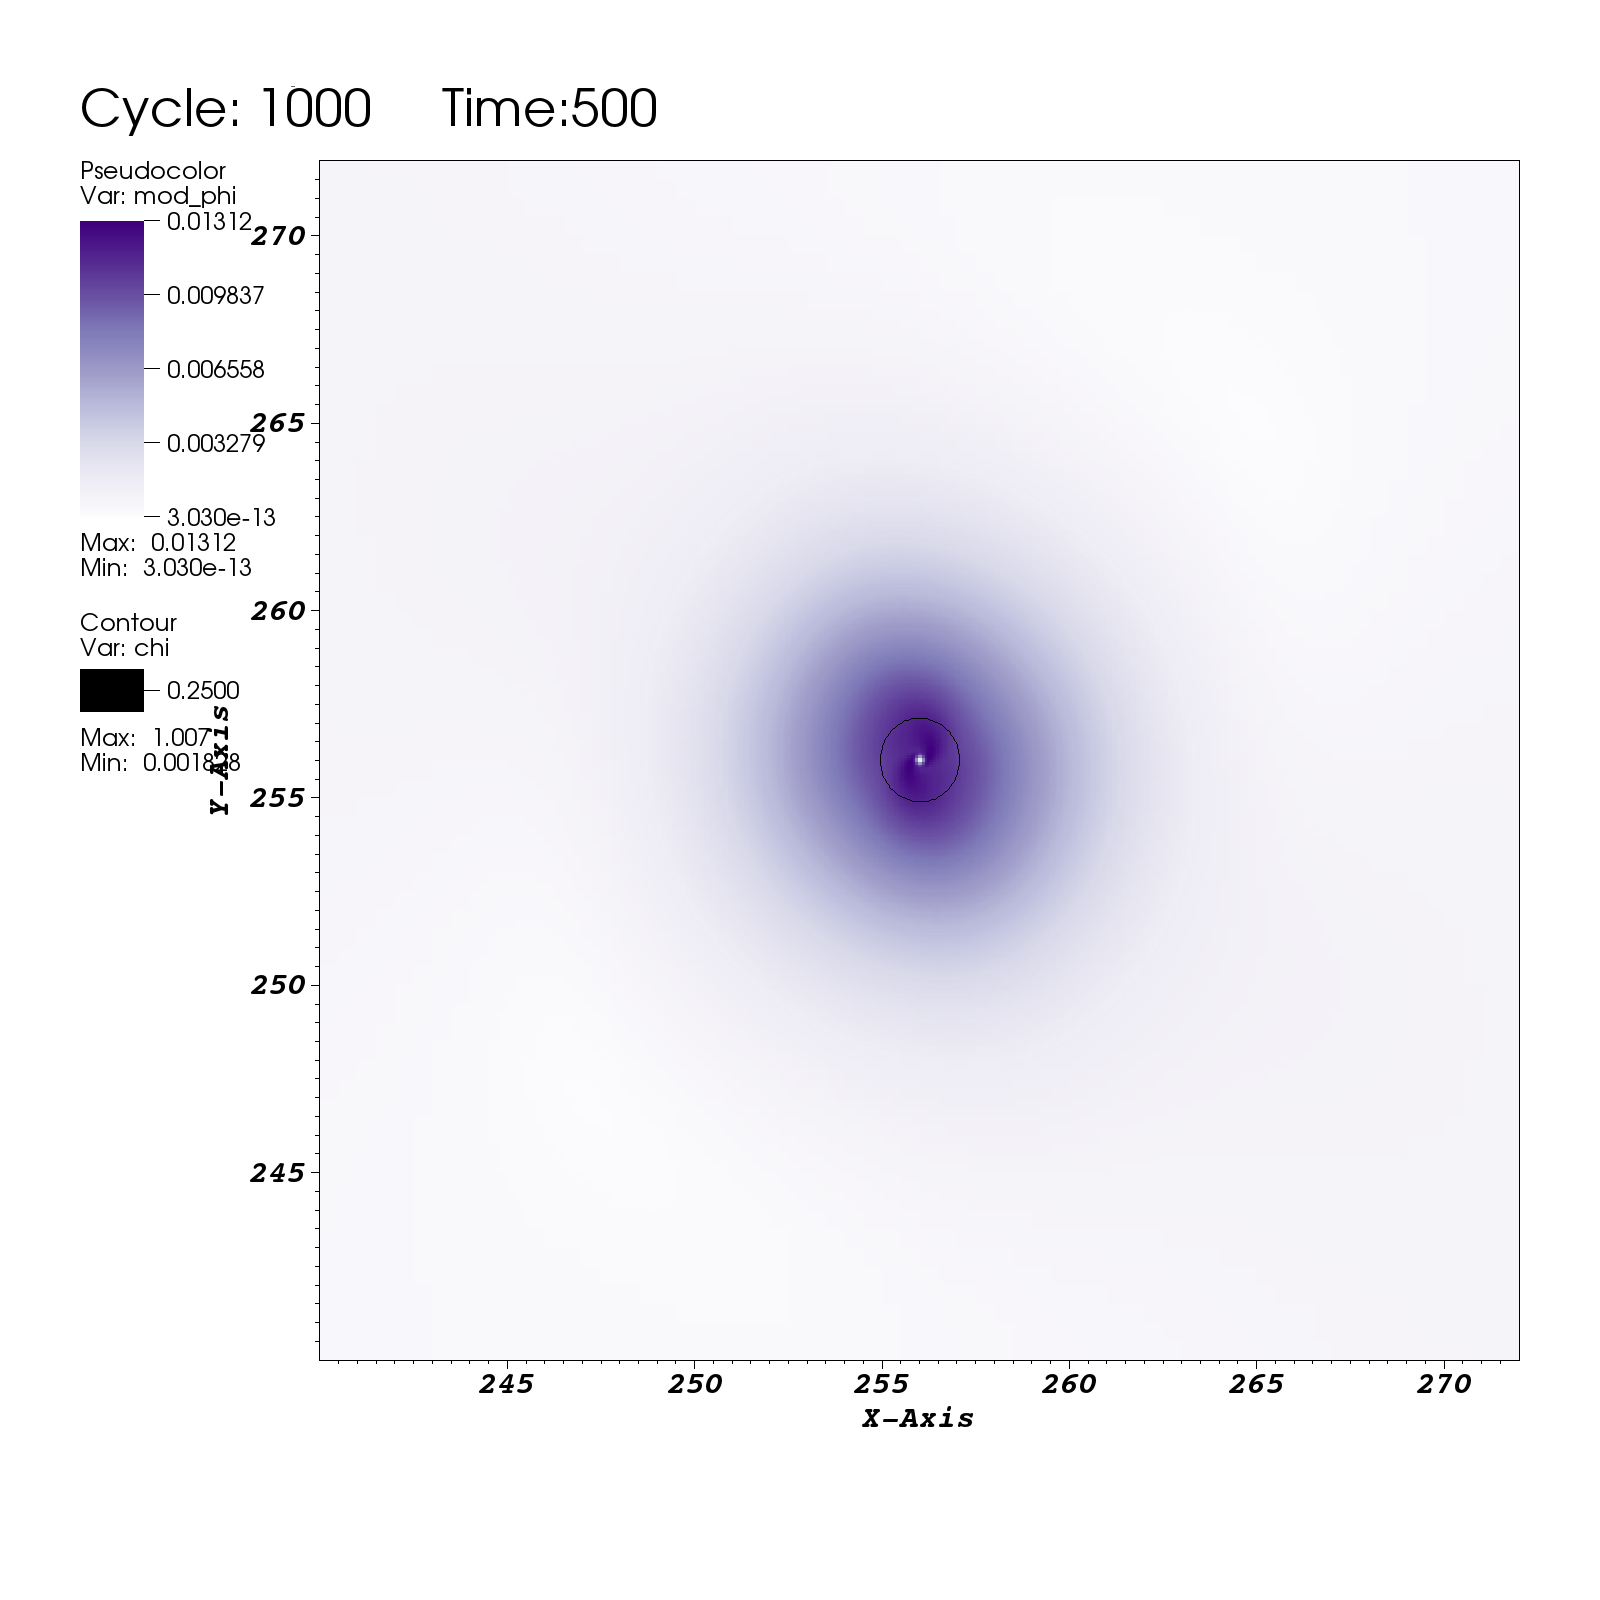
\includegraphics[width=0.45\textwidth]{modphi/graze_mod_phi0020.png}}
% \end{figure}








% THIS WAS ALWAYS UNCOMMENTED, STUFF ABOVE HERE MIGHT BE USEFUL
% THIS WAS ALWAYS UNCOMMENTED, STUFF ABOVE HERE MIGHT BE USEFUL
% THIS WAS ALWAYS UNCOMMENTED, STUFF ABOVE HERE MIGHT BE USEFUL
% THIS WAS ALWAYS UNCOMMENTED, STUFF ABOVE HERE MIGHT BE USEFUL
% THIS WAS ALWAYS UNCOMMENTED, STUFF ABOVE HERE MIGHT BE USEFUL
% THIS WAS ALWAYS UNCOMMENTED, STUFF ABOVE HERE MIGHT BE USEFUL
% THIS WAS ALWAYS UNCOMMENTED, STUFF ABOVE HERE MIGHT BE USEFUL
% THIS WAS ALWAYS UNCOMMENTED, STUFF ABOVE HERE MIGHT BE USEFUL
% THIS WAS ALWAYS UNCOMMENTED, STUFF ABOVE HERE MIGHT BE USEFUL
% THIS WAS ALWAYS UNCOMMENTED, STUFF ABOVE HERE MIGHT BE USEFUL
% THIS WAS ALWAYS UNCOMMENTED, STUFF ABOVE HERE MIGHT BE USEFUL










































% \newpage
% \newpage
% \newpage
% \newpage
% \newpage
% \newpage
% \newpage

% \subsection{After Here is Basically Junk}

% \subsection{Head-on Collisions}
% All the cases studied here are for stationary initial data $\tilde{\A}_{ij}=0,\K=0$ in-falling from an initial separation of $d \cdot m = 32$ due to gravitational attraction. Firstly we consider the equal mass Boson star binary, initial data in figure (). At first they slowly infall creating a short lived object with three maxima, shown in figure (,left), then collapse to a black hole with a decaying spherical harmonic cloud (figures ) outside. As with all the simulations from now on we assume a black hole forms if $\chi \ll 16^{-1}$ where $\chi=16^-1$ is the value taken on the horizon for the isotropic Schwarzschild metric.
%   \begin{figure}[h!]
%   \caption{Initial Data, Left: $\chi$, Right: $|\vp|$.}
%   \centering
%   \subfloat{\includegraphics[width=0.5\textwidth]{headon_bs/chi0000.png}\label{boson:fig:f9}}
%   \hfill
%   \subfloat{\includegraphics[width=0.5\textwidth]{headon_bs/modphi0000.png}\label{boson:fig:f10}}
% \end{figure}
%   \begin{figure}[h!]
%   \caption{Scalar field amplitude before and after black hole formation, Left: Time $t\cdot m = 150$, Right: Time $t \cdot m = 200$.}
%   \centering
%   \subfloat{\includegraphics[width=0.5\textwidth]{headon_bs/modphi0003.png}\label{boson:fig:f11}}
%   \hfill
%   \subfloat{\includegraphics[width=0.5\textwidth]{headon_bs/modphi0004.png}\label{boson:fig:f12}}
% \end{figure}
%    \begin{figure}[h!]
%   \caption{Real part of scalar field after black hole formation, Left: xy plane, Right: yz plane, perpendicular to initial star separation.}
%   \centering
%   \subfloat{\includegraphics[width=0.5\textwidth]{headon_bs/phi_re0004.png}\label{boson:fig:f13}}
%   \hfill
%   \subfloat{\includegraphics[width=0.5\textwidth]{headon_bs/phi_re_perp0004.png}\label{boson:fig:f14}}
% \end{figure}

% The second case considered is the same Boson star outside a black hole parameterised by $M=10M_{BS}$ where $M_{BS}$ is the ADM mass of the Boson star. The scalar field tidally deforms into an ellipsoid with high central density, well beyond Kaup limit of $\vp(0)\sim 0.0764$, and spontaneous collapse to a smaller external black hole is observed. After collapse, figure (), there is an elongated cloud about the new small black hole; there are many nodal lines in $\mathrm{Re}(\vp)$ which focus on the large black hole showing the cloud is in-falling.

%   \begin{figure}[h!]
%   \caption{Initial Data, Left: $\chi$, Right: $|\vp|$.}
%   \centering
%   \subfloat{\includegraphics[width=0.5\textwidth]{LMR/chi0000.png}\label{boson:fig:f15}}
%   \hfill
%   \subfloat{\includegraphics[width=0.5\textwidth]{LMR/modphi0000.png}\label{boson:fig:f16}}
% \end{figure}
%   \begin{figure}[h!]
%   \caption{Final Data at time $t\cdot m = 125$, Left: Conformal factor $\chi$, Right: Scalar field modulus $|\vp|$, Bottom: Real part of scalarfield $\mathrm{Re}(\vp).$}
%   \centering
%   \subfloat{\includegraphics[width=0.5\textwidth]{LMR/chi0005.png}\label{boson:fig:f17}}
%   \hfill
%   \subfloat{\includegraphics[width=0.5\textwidth]{LMR/modphi0005.png}\label{boson:fig:f18}}
%   \\
%    \subfloat{\includegraphics[width=0.5\textwidth]{LMR/phi_re0000.png}\label{boson:fig:f19}}
% \end{figure}
% Final case consists of an equal mass Black Hole and Boson Star, initial configuration in Figure 11. As can be seen from the plot of $\Re(\phi)$ and $|\phi|$, in Figure 12, most of the star falls into the black hole, however some scalar field manages to excite an intricate spherical harmonic cloud pattern.
%   \begin{figure}[h!]
%   \caption{Initial data for equal mass Boson Star and Black Hole, Left: $\chi$, Right: $|\vp|$}
%   \centering
%   \subfloat{\includegraphics[width=0.5\textwidth]{headon/chi0000.png}\label{boson:fig:f20}}
%   \hfill
%   \subfloat{\includegraphics[width=0.5\textwidth]{headon/mod_phi0000.png}\label{boson:fig:f21}}
% \end{figure}
%   \begin{figure}[h!]
%   \caption{Time $t\cdot m=905$ for equal mass Boson Star and Black Hole, Left: $\Re(\vp)$, Right: $|\vp|$}
%   \centering
%   \subfloat{\includegraphics[width=0.5\textwidth]{headon/phi_re0000.png}\label{boson:fig:f22}}
%   \hfill
%   \subfloat{\includegraphics[width=0.5\textwidth]{headon/mod_phi0007.png}\label{boson:fig:f23}}
% \end{figure}

% In all three cases, the Noether charge drops rapidly upon the formation of a black hole; this will be explained in the next section. However some scalar field lingers after collapse, in each case the hair takes the form of spherical harmonics discussed in (). Also observed is the decay of the spherical harmonics to zero amplitude in these simulations with no angular momentum.

% \subsection{Binary Inspiral}
% The only considered case here is the Quasi-circular orbit and inspiral of two equal mass boson stars. The initial boosts were determined by a newtonian calculation yielding
% \begin{equation} v^2 = \frac{M}{2d}\end{equation}
% where $M=0.53(29)$ is the ADM mass of the Boson Star and d is the initial separation. For a relatively low separation of $d\cdot m =32$ code units, shown in Figures 13,14 (Left), we get $v \sim 0.0915$. The boson stars are observed to complete roughly half an orbit before merging and collapse, forming a black hole. Here a Kerr black hole is assumed to have formed as the spacetime has a significant angular momentum which should partially infall with the scalar field.

%   \begin{figure}[h!]
%   \caption{Boson Star $|\vp|$. Left: initial data, Right: later time $t \cdot m = 700$}
%   \centering
%   \subfloat{\includegraphics[width=0.5\textwidth]{inspiral/mod_phi_inspiral_nice0000.png}\label{boson:fig:f24}}
%   \hfill
%   \subfloat{\includegraphics[width=0.5\textwidth]{inspiral/mod_phi_inspiral_nice0002.png}\label{boson:fig:f25}}
% \end{figure}
%   \begin{figure}[h!]
%   \caption{Boson Star $\Re(\vp)$. Left: initial data, Right: later time $t \cdot m = 700$}
%   \centering
%   \subfloat{\includegraphics[width=0.5\textwidth]{inspiral/phi_inspiral_nice0000.png}\label{boson:fig:f26}}
%   \hfill
%   \subfloat{\includegraphics[width=0.5\textwidth]{inspiral/phi_inspiral_nice0002.png}\label{boson:fig:f27}}
% \end{figure}
%   \begin{figure}[h!]
%   \caption{Left: Total Noether charge $\mathcal{N}$ during evolution, Right: $\Psi_4$ over 22 harmonic during evolution.}
%   \centering
%   \subfloat{\includegraphics[width=0.5\textwidth]{inspiral/N.png}\label{boson:fig:f28}}
%   \hfill
%   \subfloat{\includegraphics[width=0.5\textwidth]{inspiral/GW.png}\label{boson:fig:f29}}
% \end{figure}
% Figure 15 shows the total Noether charge, which is no longer conserved. When the black hole forms, the in-falling scalar field moves towards zero radius and gets hugely compressed. The huge compression causes extreme field gradients which induces continuous regridding in the AMR, but this is capped at 7 layers in this simulation to make runtime feasible. When the 8th AMR level is needed it is simply not added and resolution becomes low enough that any Noether charge near the centre is so under-resolved that it seems to fall between the gridpoints. Interestingly, Figures 13,14 (Right) show a scalar field configuration lingering around the black hole, mostly outside the contour $\chi=0.7$, looking like scalar hair. Also Figure 15 (Left) of the Noether charge appears to take significantly longer to decay than in the linear collision simulations. It can be seen in Figure 14 in the plot of $\Re(\vp)$ that the cloud has angular nodes corresponding to angular momentum similarly to boosted stars picking up nodal planes perpendicular to momentum and Figure 10 (Bottom) of the infalling cloud.

% The gravitational wave (GW) signal can be seen in Figure 15 (Right), extracted at a radius $r \cdot m = 90$. At the time $t \cdot m \approx 700$ the gravitational wave signal due to the merger appears; in order to record a longer inspiral simulations with larger initial separations need to be simulated. Currently there appears to be some small problem with the initial data, also observed in the collisions with no angular momentum, that manifests itself in noisy GW extraction and the Hamiltonian constraint initially sharply rising.
